\documentclass[11pt]{book}

\usepackage[T1]{fontenc}
\usepackage{hyperref}
\usepackage{microtype}
\usepackage{lettrine}

\usepackage{standalone}
\usepackage{pgfplots}
\pgfplotsset{compat=1.17}
\usepgfplotslibrary{groupplots}
\usepgfplotslibrary{fillbetween}
\usetikzlibrary{fadings}

\usepackage[commands,environments,enumerate,citations,notes,a4paper]{AVT}

\bibliography{citations}

\title{Gaussian Processes and Statistical Decision-making in Non-Euclidean Spaces}
\author{Alexander Terenin}
\date{August 2021}

\begin{document}

\begin{titlepage}
\maketitlehooka
\centering
\huge
\null
\vfill
\thetitle
\par
\vfill
\LARGE
\theauthor
\par
\large
Department of Mathematics
\par
Imperial College London
\par
\vfill
\null
\vfill
a dissertation submitted for the degree of
\par
Doctor of Philosophy
\par
\strut
\par
\thedate
\par
\vfill
\null
\maketitlehookd
\end{titlepage}

\chapter*{Declaration}

No more than 100,000 words

\chapter*{Copyright}

The copyright of this thesis rests with the author. Unless otherwise indicated, its contents are licensed under a Creative Commons Attribution 4.0 International Licence (CC BY).

Under this licence, you may copy and redistribute the material in any medium or format for both commercial and non-commercial purposes. You may also create and distribute modified versions of the work. This on the condition that you credit the author.

When reusing or sharing this work, ensure you make the licence terms clear to others by naming the licence and linking to the licence text. Where a work has been adapted, you should indicate that the work has been changed and describe those changes.

Please seek permission from the copyright holder for uses of this work that are not included in this licence or permitted under UK Copyright Law.

\chapter*{Acknowledgments}

\chapter*{Abstract}

Not more than 300 words

\tableofcontents





\chapter{Introduction}
\label{ch:intro}

\lettrine{L}{earning} from experience in order to change behavior is one of the defining abilities of biological systems, which differentiates them from other kinds of systems found in the world.
Replicating the processes biological systems use to learn and adapt is a fundamental goal of science and technology.
To this end, the development of mathematical formalisms rich enough to capture the notion of learning is one of the crowning achievements of statistics, machine learning, and artificial intelligence.

One such formalism is the \emph{Bayesian} view of learning.
In this framework, one starts with (i) a probability distribution describing the information known about the quantity of interest external to the data, and (ii) a conditional probability distribution describing how the quantity of interest relates to the data.
These are combined into a joint distribution and conditioned on the specific observed data values, giving a probability distribution describing what was learned about the quantity of interest by observing the data.

The Bayesian view of learning gives rise to a theory of \emph{decision}, which describes how an abstract decision system should select actions in pursuit of a goal.
This is done by learning how different actions affect pursuit of the goal, and selecting optimal actions consistent with what was learned.
By virtue of being probabilistic, such decisions systems assess and propagate uncertainty, enabling them to balance what is already known with what could be learned by taking actions---a concept known as the \emph{explore-exploit tradeoff}.

The performance of a decision system can be evaluated by examining how quickly its decisions improve and become optimal.
A decision system's \emph{regret} is the reduction in its quality of decisions by virtue of not knowing the quantity of interest in advance.
In most non-trivial settings, one can show that some regret is inevitable: a decision-making system must make some degree of mistakes in order to learn.
A decision system is considered \emph{optimal} if its regret is within a constant factor of the best possible regret.

Decisions systems with optimal or close-to-optimal regret require less data in order to solve their respective tasks, and are called \emph{data-efficient}.
Data-efficiency is a key concern in practical settings, where data-collection takes time and can be expensive.
By virtue of resolving explore-exploit tradeoffs in a manner amenable to regret analysis, the Bayesian formalism gives broad tools for constructing data-efficient decision systems.

The key limitation of the Bayesian approach is that it is often \emph{too powerful}, and leads to computational problems which are intractable.
Conditional distributions generally contain more information than actually needed to make optimal decisions, yet calculating them is largely unavoidable.
Probabilistic decision systems are thus most attractive settings where their strengths---including data-efficiency, solid technical foundations, and amenability to analysis---can shine, while computational costs are kept under control.

In my view, \emph{Gaussian processes} are one such setting: they are powerful enough to model wide classes of unknown quantities of interest, yet their computational costs are generally polynomial.
Better yet, Gaussian-process-based decision systems have been demonstrated to exhibit excellent performance in a number of practical settings, including ones deployed in real-world scientific applications.
Studying Gaussian processes is therefore a promising avenue towards improved understanding of Bayesian learning and Bayesian decision-making in pursuit of artificial intelligence.

The goals of this dissertation are twofold: (i) to make Gaussian processes easier to work with through improved numerical methods, particularly in cases where they are used within larger decision systems, and (ii) to expand the set of settings where Gaussian processes can be practically employed in, enabling construction of decision systems for applications not previously considered.
Contributions toward (i) include path-wise conditioning techniques studied in \Cref{ch:pathwise}, and contributions toward (ii) include non-Euclidean Gaussian processes studied in \Cref{ch:noneuclidean}.
Following these, \Cref{ch:conclusion} concludes.

To pursue these goals, it is critically important that all of the concepts described in the preceding paragraphs be made into rigorous mathematics, so that the ideas described in the sequel ultimately reduce to definitions and implications, and not metaphor or opinion.
Together, we therefore begin by defining the key mathematical notions needed.

\section{Bayesian learning}

The first concept we develop in depth along our path towards a mathematically precise understanding of statistical decision-making will be \emph{Bayesian learning}---a mathematical formalism for reasoning about unknown quantities of interest on the basis of data.
Bayesian learning is a \emph{probabilistic} theory: a model specifies how the quantity of interest and the data depend on one another as random variables.
Learning then entails calculating how the distribution of the quantity of interest changes upon observing the data.

One of the key strengths of Bayesian theory is that it applies in very wide generality, owing to the substantial scope of probability theory. 
In particular, one can consider unknown quantities of interest that are function-valued, and study learning in such settings.
This, however, requires a non-elementary treatment, as one cannot rely solely on probability densities to define what conditional distributions are.
We therefore begin by recalling the necessary formalism.

\subsection{Review of probability theory}
We adopt the language of measure-theoretic probability, which we now describe.
To ease presentation, we state the definitions together with useful ways of thinking about them.


We say that \emphmarginnote{measurable space} is a pair $(Y,\c{Y})$ consisting of a set $Y$ and a $\sigma$-algebra $\c{Y}$ over $Y$.
A \emph{$\sigma$-algebra} is a set of subsets of $Y$ containing the space itself which is closed under unions, intersections, complements, and set-theoretic monotone limits.
These can be reinterpreted as Boolean logical operations, so $\c{Y}$ can be thought of as the set of all true-false questions one can ask about elements of the set $Y$. 
These questions, then, are closed under \emph{and/or/not} operations and monotone limits thereof.

\parmarginnote{Product of measurable spaces}
Given two measurable spaces $(Y,\c{Y})$ and $(\Theta,\mathit\Theta)$, if we form the Cartesian product $Y \x \Theta$, then we can define the \emph{product $\sigma$-algebra} $\c{Y}\ox\mathit\Theta$ as the smallest $\sigma$-algebra containing all sets of the form $A_y \x A_\theta$ with $A_y \in\c{Y}$ and $A_\theta\in\mathit\Theta$.
\marginnote{Subset of a measurable space}
For a measurable subset $Y' \subseteq Y$, we can define $\c{Y}' = \{A_y \^ Y' : A_y \in\c{Y}\}$, which is also a $\sigma'$-algebra, thereby making $(Y',\c{Y}')$ into a measurable space. 
We call $\c{Y}'$ the \emph{subset $\sigma$-algebra}.

\parmarginnote{Measurable function}
A map $f : Y \-> Y'$ between measurable spaces $(Y,\c{Y})$ and $(Y',\c{Y}')$ is said to be \emph{measurable} if its preimage defines a map $f^{-1} : \c{Y}' \-> \c{Y}$ between the respective $\sigma$-algebras.
This means that true-false questions for the space $Y'$ can be asked and answered relative to true-false questions for the space $Y$.
On product spaces, a map $f : Y \-> \Theta \x \Theta'$ is measurable if its components are measurable, but a map $f : Y \x Y' \-> \Theta$ \emph{need not} automatically be measurable if $f(\.,y') : Y \-> \Theta$ and $f(y,\.) : Y' \-> \Theta$ are measurable for all $y$ and $y'$.

A \emphmarginnote{probability measure} is a countably additive map $\pi_y : \c{Y} \-> [0,1]$ satisfying $\pi_Y(Y) = 1$. 
This can be thought of as a map that takes a true/false question, and assigns a number indicating how close to true or false its answer is according to the measure---in this view, probability measures describe uncertainty.
A \emph{probability space} is a measurable space $(\Omega,\c{F})$ equipped with a probability measure $\P$.
The set $\Omega$ can be viewed as a space of abstract random numbers, with a random number generator described by $\P$.

Given a probability space, we say that a \emphmarginnote{random variable} is measurable map $y : \Omega \-> Y$.
A random variable, then, maps random numbers $\omega\in\Omega$ into the space $Y$.
The \emph{distribution}\marginnote{Distribution} of a random variable is defined as the \emph{pushforward measure} $\pi_y(A_y) = (y_* \P)(A_y) = \P(y^{-1}(A_y))$ for all $A_y\in\c{Y}$.
The probability of an event $A_y$, then, is determined by measuring the probability of random numbers under which $A_y$ occurs---measurability guarantees this is possible.

\parmarginnote{Notation for random variables}
In this work, we will generally \emph{not} adopt the standard convention of suppressing $\omega$-arguments of random variables from our notation, and will write such arguments explicitly.
Though this makes expressions slightly denser, it also avoids ambiguity and presents the mathematics more precisely.

\parmarginnote{Equality of random variables}
There are multiple senses in which we can say random variables are equal.
We say that $y = y'$ \emph{surely} if they are equal as mathematical functions.
This notion is essentially never used, because it is exceedingly strong.
We say that $y = y'$ \emph{almost surely} if $\P(y \neq y') = 0$, in which case $y$ and $y'$ are equal as functions, except possibly on a set of measure zero.
We say that $y = y'$ \emph{in distribution} if $y_* \P = y'_* \P$, meaning their distributions are equal.

\parmarginnote{Existence of a random variable with given distribution}
For a given probability space $(\Omega,\c{F},\P)$, a random variable $y : \Omega \-> Y$ with distribution $\pi_y$ need not exist.
However, if it does not, there always exists another probability space $(\Omega',\c{F}',\P')$ and a measurable map $i : \Omega' \-> \Omega$ such that $\P = i_* \P'$, and for which a $\pi_y$-distributed random variable $y : \Omega' \-> Y$ \emph{does} exist.
We will thus implicitly assume all probability spaces are large enough to ensure all random variables with prescribed distributions exist.

\parmarginnote{Probability kernel}
We will be interested in probability measures extended to allow them to be parameterized by other quantities.
A \emph{probability kernel} is defined to be a map $\pi_{y\given\theta} : \c{Y} \x \Theta \-> [0,1]$ satisfying two conditions: (i) the map $\pi_{y\given\theta}(\.,\vartheta) : \c{Y} \-> [0,1]$ is a probability measure for almost all $\vartheta\in\Theta$, and (ii) the map $\pi_{y\given\theta}(A_y,\.) : \Theta \-> [0,1]$ is measurable for all $A_y\in\c{Y}$.

\parmarginnote{Conditional distribution}
Random variables can also be extended to parameterize them by other quantities.
A $\c{F}\ox \mathit\Theta$-measurable map $y\given\theta : \Omega \x \Theta \-> Y$ is called a \emph{jointly measurable stochastic process}---we largely eschew this terminology to emphasize the Bayesian nature of our formalism.
In particular, unlike most presentations of stochastic processes, we \emph{never} think of $\Theta$ as representing time.
Define the \emph{conditional distribution} of $y\given\theta$ to be $(y\given\theta)_*\P$, with the pushforward taken in the first argument---by \Cref{lem:rcrv-rvm-equiv}, this is a probability kernel.


\subsection{Bayes' Rule for probability measures}

The key idea behind Bayesian learning is to formalize \emph{learning} using the concept of \emph{conditional probability}.
This entails (i) building a model entails quantifying the relationship between the \emph{quantity of interest} $\theta$, and the \emph{data} $y$, and (ii) quantifying what is learned using Bayes' Rule.
We now begin to make these concepts precise in the language of measure-theoretic probability.

\begin{definition}[Bayesian model]
Let $Y$ and $\Theta$ be sets.
A \emph{Bayesian model} is a probability measure defined on $\Theta \x Y$.
\end{definition}

A model can be constructed in a number of different ways.
The most common technique is to specify two components: (i) a probability distribution describing what is known about the quantity of interest external to the data, and (ii) how the data relates to the quantity of interest.
These are called the \emph{prior distribution} and \emph{likelihood}, respectively.

\begin{proposition}
A Bayesian model can be constructed in the following ways.
\1 Using measures: integrate the following two components.
\1 \emph{Prior}: a probability measure $\pi_\theta$.
\2 \emph{Likelihood}: a probability kernel $\pi_{y\given\theta}$.
\0 
\2 Using random variables: compose the following two components.
\1 \emph{Prior}: a random variable $\theta:\Omega\->\Theta$.
\2 \emph{Likelihood}: a jointly measurable stochastic process $y\given\theta: \Omega\x\Theta\->Y$.
\0 
\0 
Moreover, if $y\given\theta$ additionally satisfies the \emph{non-duplicate dependence} condition---namely, that for almost every $\theta'\in\Theta$, the random variable $(y\given\theta)(\.,\theta') : \Omega \-> Y$ is independent of $\theta$---then the constructions coincide.
\end{proposition}

\begin{proof}
For the former, define 
\[
\pi_{\theta,y}(A_\theta\x A_y) = \int_{A_\theta} \pi_{y\given\theta}(A_y\given\theta) \d\pi_\theta(\theta)
\]
which extends to the full product $\sigma$-algebra by \Cref{lem:cyl-prod}, giving the desired probability measure.
For the latter, define the random variable
\[
\gamma : \Omega &\-> \Theta \x Y
&
\gamma : \omega &\|> (\theta(\omega), (y\given\theta)(\omega,\theta(\omega)))
\]
and take $\pi_{\theta,y} = \gamma_* \P$. 
We now prove these expressions coincide.
Write 
\[
\pi_{\theta,y}(A_\theta\x A_y) &= \int_{A_\theta} \pi_{y\given\theta}(A_y\given\theta) \d\pi_\theta(\theta)
\\
&= \int_\Omega\1_{\theta(\omega)\in A_\theta} \pi_{y\given\theta}(A_y\given\theta(\omega)) \d\bb{P}(\omega)
\\
&= \int_\Omega\1_{\theta(\omega)\in A_\theta} \int_\Omega \1_{(y\given\theta)(\omega',\theta(\omega)) \in A_y} \d\bb{P}(\omega') \d\bb{P}(\omega)
\\
&= \int_{\Omega\x\Omega} \1_{(\theta(\omega),(y\given\theta)(\omega',\theta(\omega))) \in A_\theta \x A_y} \d\bb{P}^2(\omega,\omega')
\\
&= \int_\Omega \1_{(\theta(\omega),(y\given\theta)(\omega,\theta(\omega))) \in A_\theta \x A_y}\d\bb{P}(\omega)
\\
&= \P((\theta,(y\given\theta)(\.,\theta)) \in A_\theta \x A_y)
\]
which follows using Tonelli's Theorem, \Cref{lem:cyl-prod}, and \Cref{lem:non-dupl-dep} via the non-duplicate dependence condition.
\end{proof}

These two components should be interpreted as follows: $\theta$ describes what is known about the quantity of interest external to the data, and $y\given\theta$ describes how the data $y$ relates to the quantity of interest.
More specifically, the likelihood describes how $y$ would be distributed if $\theta$ was known and equal to the conditioned value.

Given a Bayesian model, we can formalize the notion of what is \emph{learned} about $\theta$ from observing $y$ as its conditional probability distribution---note that this is meant in a \emph{distributional} sense, not a random-variable-based sense.
The formulation is given as follows.

\begin{figure*}[t]
\vspace*{10ex}
[Bayes' Rule 3D Visual]
\vspace*{10ex}
\caption{TODO.}
\end{figure*}

\begin{result}[Bayes' Rule]
Suppose that $\Theta$ and $Y$ are second-countable topological spaces, and let $\pi_y = \pi_{\theta,y}(\Theta\x\.)$.
Then for every Bayesian model $\pi_{\theta,y}$ there is a $\pi_y\ae[-]$ unique probability kernel $\pi_{\theta\given y}$, which we call the \emph{posterior distribution}.
\end{result}

\begin{proof}
Apply the Disintegration Theorem.
\end{proof}

This result shows that given a Bayesian model, the posterior distribution \emph{exists}.
In its full abstract formulation, however, Bayes' Rule is \emph{non-constructive}, and it is not at all clear how to calculate any kind of useful formula from it.
Fortunately, in many settings this is possible by virtue of additional structure.

The simplest such structure occurs when $\pi_{\theta,y}$ admits a density with respect to a reference measure $\lambda$.
In this case, it follows \Cref{lem:prod-density} that $\pi_\theta$ admits the density $f_\theta$ with respect to $\lambda(\.\x Y)$, and similarly for $\pi_y$ and $f_y$.
Define a \emph{conditional density} as the ratio of joint and marginal densities, and let $\propto$ denote equality up to a proportionality constant.
Then we have the following.

\begin{proposition}[Bayes' Rule for densities]
Suppose that $\pi_{\theta,y}$ admits the density $f_{\theta,y}$ with respect to $\lambda_{\theta,y}$.
Then we have
\[
f_{\theta\given y} \propto f_{y\given\theta}f_\theta
.
\]
\end{proposition}

\begin{proof}
We have
\[
f_{\theta,y} &= \frac{f_{\theta,y}}{f_\theta} f_\theta = f_{y\given\theta}f_\theta
&
f_{\theta,y} &= \frac{f_{\theta,y}}{f_y} f_y = f_{\theta\given y}f_y
\]
which, when combined, give the result.
\end{proof}

Sometimes, the knowledge of $f(\theta\given y)$ up to proportionality is enough to fully deduce its form.
For example, if the likelihood is Gaussian with unknown mean and known variance, and the prior is also Gaussian, then the posterior is Gaussian.
In cases such as this, the pair $(\pi_{y\given\theta}, \pi_\theta)$ are called \emph{conjugate}.

Bayes' Rule for densities is remarkable in its generality yet restrictiveness.
On one hand, we require no direct assumptions about the spaces $\Theta$ and $Y$, and in particular allow real spaces, discrete spaces, and Riemannian manifolds.
On the other hand, other than in the aforementioned settings, where we can employ the Lebesgue, counting, and Riemannian volume measures, respectively, finding a suitable reference measure can be difficult.

We will work with posterior distributions in infinite-dimensional vector spaces in the sequel---there, densities are either not available or not convenient.
In those cases, it is enough to calculate the posterior on arbitrary finite-dimensional marginal projections to uniquely determine its value on the full infinite-dimensional space.

\begin{proposition}[Conditioning and marginalization]
Conditioning and marginalization commute.
\end{proposition}

\begin{proof}
TODO.
\end{proof}

This result makes densities into a substantially more powerful tool than they would be otherwise, since it enables us to use them for calculating posterior distributions even where they are not directly available.
In particular, we can map an infinite-dimensional function space into finite-dimensional vector spaces induced by pointwise function evaluations at arbitrary points, enabling us to calculate posterior distributions in such settings, in spite of no suitable densities existing directly in the space of interest.

We now introduce the \emph{variational formulation} of Bayes' Rule, which expresses the posterior as the solution to an infinite-dimensional optimization problem.

\begin{proposition}[Bayes' Rule in variational form]
\label{prop:variational-bayes}
Assume TODO.
Then for every $\gamma\in Y$, the posterior distribution satisfies 
\[
\pi_{\theta\given y}(\.\given \gamma) = \argmin_{\bb{q}_\theta \in \c{M}_1(\Theta)} D_{\f{KL}}(\bb{q}_\theta \from \pi_\theta) - \operatorname*{\E}_{\vartheta\~\bb{q}_\theta} \ln f_{y\given\theta}(\gamma\given\vartheta)
\]
where the minima does not depend on the choice of reference measure used in defining the likelihood density.
\end{proposition}

\begin{proof}
We prove the result twice, using two different techniques---by computations that involve Kullback--Leibler divergences, and by employing ideas from the calculus of variations.
We start with the former. 
Since the topology generated by the Kullback--Leibler divergence on the space of probability measures is Hausdorff, we have
\[
\pi_{\theta\given y}(\.\given \gamma) &= \argmin_{\bb{q}_\theta \in \c{M}_1(\Theta)} D_{\f{KL}}(\bb{q}_\theta \from \pi_{\theta\given y}(\.\given \gamma))
\]
TODO
\end{proof}

For any given dataset, this result shows that  Bayes' Rule can be viewed in \emph{information-theoretic} manner: among all probability measures, the posterior maximizes predictive power, while retaining as many bits as possible from the prior, in the sense given by the Kullback--Leibler divergence.

The result also suggests a way to approximately compute posterior distributions: solve the optimization problem on a suitably chosen subspace of the space of all probability measures $\c{M}_1(\Theta)$.
This strategy will be particularly fruitful in the later-described setting of Gaussian processes, where techniques for constructing such approximations with well-understood and favorable accuracy will be considered.

We will \emph{always} view variational approximations as minimization of Kullback--Leibler divergences, as this is mathematically sound.
We will eschew standard presentations involving \emph{evidence lower bounds}: the only mathematical explanations for why maximizing these bounds should improve model performance, that I am aware of, appeal to Kullback--Leibler divergences---so, then, why talk about evidence lower bounds in the first place?

Once a posterior is calculated, the next step is to extract the relevant quantities from it.
Traditionally, this is often done by displaying summary statistics to be evaluated and interpreted by a person with statistical training, often with a focus on assessing uncertainty.
We will instead focus on settings where the posterior is given as input to an upstream decision-making algorithm: we explore these next.

\subsection{Technical lemmas}

We now prove a number of technical lemmas used in the preceding text, which for completeness are presented here in order to avoid disrupting the reader's flow.

\begin{lemma}
\label{lem:rcrv-rvm-equiv}
Let $b:\Omega\x A\->B$ be a jointly measurable stochastic process.
Then the map $b_*\P : \c{B} \x A \-> [0,1]$, where the pushforward is taken in the first argument, is a probability kernel.
\end{lemma}

\begin{proof}
It is clear that $b_* \P$ is a probability measure for all $a'\in A$, so we only need to prove that the map $a \|> (b(\.,a)_*\P)(A_b)$ is measurable for all $A_b\in\c{B}$.
First, write
\[
(b_*\P)(A_b) = \P(b(\.,a)^{-1}(A_b)) = \int_\Omega \1_{b(\omega,a)\in A_b} \d\bb{P}(\omega)
.
\]
Now, note that the map $\Omega\x A\->\R$ given by $(\omega,a) \|> \1_{b(\omega,a)\in A_b}$ is bounded measurable, since $b$ is measurable in both arguments, and indicators of measurable functions on measurable sets are bounded measurable.
Finally, since for any bounded measurable $f : \Omega \x A \-> \R$, the map $a \|> \int_\Omega f(\omega,a) \d\bb{P}(\omega)$ is measurable by Fubini's Theorem, the claim follows.
\end{proof}

\begin{lemma}
\label{lem:cyl-prod}
Let $\pi : \c{A} \x \c{B} \-> [0,1]$ be a function satisfying the measure axioms.
Then $\pi$ extends uniquely to a measure on the product sigma-algebra.
\end{lemma}

\begin{proof}
Apply a $\pi$-$\lambda$ argument.
TODO.
\end{proof}

\begin{lemma}
\label{lem:non-dupl-dep}
Let $a : \Omega \-> A$ be a random variable and $b : \Omega \x A \-> B$ be a jointly measurable stochastic process.
Suppose that for almost all $a'\in A$, the random variable $b(\.,a') : \Omega \-> B$ is independent of $a$.
Then for all bounded measurable functions $f$ we have
\[
\int_\Omega f(a(\omega),b(\omega,a(\omega))) \d\bb{P}(\omega) = \int_{\Omega\x\Omega}f(a(\omega),b(\omega',a(\omega))) \d\bb{P}^2(\omega,\omega')
.
\]
\end{lemma}

\begin{proof}
TODO.
\end{proof}

\begin{lemma}
\label{lem:prod-density}
Let $\pi_{a,b}$ be a measure which admits a density with respect to $\lambda$.
Then $\pi_{a,b}(\.\x B)$ admits a density with respect to $\lambda(\.\x B)$, and similarly in the other argument.
\end{lemma}

\begin{proof}
Apply a Fubini-type argument.
TODO.
\end{proof}

\section{Statistical decision-making}

We now use the Bayesian formalism to construct a probabilistic theory of decision-making.
To begin, we formalize the very general concept of an abstract agent making decisions in an environment in pursuit of some goal.

\subsection{Markov decision processes}

\begin{definition}[Discrete-time Markov decision process]
A \emph{discrete-time Markov decision process} is a $4$-tuple consisting of the following.
\1 State space: a measurable space $S$.
\2 Action space: a measurable space $A$.
\3 Reward: a probability kernel $r : \c{B}(\R) \x X \x A \-> \R$. 
\4 Transition kernel: a probability kernel $p : \c{S} \x S \x A \-> \R$.
\0 
\end{definition}

This is a very broad notion---however, a number of variations are also possible.
For instance, one can consider continuous-time, purely deterministic, and partially observed analogs---each of these involve their own subtleties and deserve study in their own right, but we do not pursue them here.

\begin{figure*}[t]
\vspace*{10ex}
[Markov Decision Process Visual Diagram]
\vspace*{10ex}
\caption{TODO.}
\end{figure*}

The idea behind this definition is that, at every point in time, the agent observes the current state, chooses an action $a \in A$, and obtains another state $s' \~ p(s,a)$.
Note that \emph{time} can, and often will, be part of the state $s$.
The agent's goal is to choose each action so as to control the entire trajectory of states in order to obtain maximum rewards.
The choice of actions in every state is called a \emph{policy}, and is formalized as follows.

\begin{definition}[Policy]
Define the following.
\1 A measurable function $\pi : S \-> A$ is called a \emph{deterministic policy}.
\2 A probability kernel $\pi : \c{A} \x S \-> \R$ is called a \emph{Markov policy}.
\0 
\end{definition}

Markov policies include deterministic policies as a special case, by taking the conditional distributions to be Dirac and re-interpreting the given expressions appropriately.
As with Markov decision processes, here one can also consider even more general policies, but we do not do so here.

Different policies yield different state trajectories, and therefore different rewards.
Of these, some obtain more rewards than others: 

\begin{definition}[Optimal policy]
Let $T \in \N$ be the \emph{time horizon}.
A policy is called \emph{optimal} if it maximizes the \emph{value function} 
\[
V^{(\pi)}(x_0) = \E \sum_{t=0}^T r_t
\]
where $r_t \given s_t,a_t \~ r(s_t,a_t)$, $a_t \given s_t \~ \pi(s_t)$, and $s_{t+1} \given s_t,a_t \~ p(s_t, a_t)$.
\end{definition}

Finding an optimal policy therefore amounts to selecting the best possible actions to maximize total rewards.
It is therefore of key interest to find an optimal policy, if one exists.
Note that closely-related alternative notions of optimality, such as minimizing infinite discounted sums, or limits of averages, are also possible.
The most important distinction between different problems for finding optimal policies is given by what is assumed known.

\1 If $p$ and $r$ are known, we say we have an \emph{optimal control} problem.
\2 Otherwise, we say we have an \emph{decision} problem.
\0 

These classes differ fundamentally from one another. 
Optimal control problems can be viewed as a class of structured optimization problems, where the goal is to compute $\pi$ by evaluating $r$ and $p$ as necessary.
Here, one generally proceeds by proving that $V^{(\pi)}$ and $\pi$ satisfy certain recursive equations, and developing schemes for solving them.

Decision problems do not behave in this manner.
Due to the rewards or dynamics being \emph{unknown}, they cannot simply be maximized and their expectation must be \emph{learned}.
This forces one to consider whether to take advantage of actions known to be good, or to try others in case they might be better---this is known as the \emph{explore-exploit tradeoff}.
For such settings, we need an appropriate solution concept---to obtain one, define the following.

\begin{definition}[Regret]
The \emph{regret} of a policy $\pi$ is defined as 
\[
R^{(\pi)}(x_0) = V^*(x_0) - V^{(\pi)}(x_0)
\]
where $V^*$ is the optimal value function, which is assumed to exist.
\end{definition}

Minimizing regret is equivalent to maximizing value, but when $p$ and $r$ are unknown doing so directly is impossible.
Instead, the goal is to find an \emph{algorithm}---that is, a way of updating the policy based on observed data---so as to limit growth of regret.

In most settings, one can prove that every algorithm which does not know $p$ and $r$ necessarily incurs some level of regret.
This is done by exhibiting a randomized set of problems and rewards over which regret is lower-bounded in expectation for any algorithm.
In such a class, actions that perform well on one problem will necessarily perform badly on another problem.
Such arguments show that some degree of regret is inevitable.

On the other hand, some algorithms incur more regret than others.
The obviously-bad algorithm which learns nothing and chooses the exact same action over and over again incurs at most linear regret.
An algorithm is said to \emph{solve} a decision problem if its asymptotic regret rate with respect to $T$ matches the respective regret lower bound in the given problem class.
Finding such algorithms is of key interest.

One way to construct algorithms for solving decision problems is to employ a \emph{model-based} approach, which loosely speaking works as follows.

\1 Learn the unknown transitions and/or rewards from observed data using a supervised learning approach.
\2 Use the learned model(s) to find policy satisfying some criteria.
\0 

The details of such approaches depends on the setting.
We distinguish between two key kinds of decision problems.

\1 If $|S| = 1$, it is known as a \emph{multi-armed bandit} problem.
\2 Otherwise, it is known as a \emph{reinforcement learning} problem.
\0 

Multi-armed bandits possess no variable state, and thus only require one to learn the rewards and determine which actions are optimal.
Reinforcement learning allows actions to influence transitions between states, and requires long-term planning, making it much more general, difficult, and important.
I believe that as a mathematical theory, reinforcement learning is powerful enough to describe many aspects of human and animal intelligence, making it a fundamentally interesting theory to study and develop.

We now restrict ourselves to the bandit setting, which is substantially easier to study and so can be understood much more deeply.
Here, even when $A$ is a finite set and the rewards are Gaussian, the model-based approach consisting of (i) estimating rewards using empirical risk minimization and (ii) choosing the policy which maximizes rewards is known to be non-optimal.
This approach fails to explore, and can get stuck chasing sub-optimal rewards.

One way to fix this problem is to replace empirical risk minimization with Bayesian learning, and adopt an appropriate decision rule for selecting actions.
Doing this yields approaches which can be shown optimal in many settings.
We therefore proceed to study multi-armed bandits in more detail.

\subsection{Multi-armed bandits}

The multi-armed bandit problem takes its name from a casino analogy.
In the 1950s, slot machines often had levers one could pull instead of buttons one could press, and were called \emph{one-armed bandits} for their ability to empty gamblers' wallets.
A \emph{multi-armed bandit} is a slot machine which for a fixed cost, allows one to pull an arm $x \in X$, and receive a random reward whose distribution depends on $x$.
The goal is to minimize  expected loss, or, equivalently, maximize total expected rewards.

Multi-armed bandits can be viewed as discrete-time Markov decision processes with a one-element state space, but this is not necessarily the most fruitful way to think about them.
We thus begin by introducing formalism and notation better suited to the given setting, which can be viewed as special cases of the notions considered previously.

\begin{figure*}[t]
\vspace*{10ex}
[Multi-armed Bandit Plot]
\vspace*{10ex}
\caption{Here, we illustrate a simple three-armed bandit. 
Each of the three arms has its own reward distribution, shown on the left.
These are unknown to the agent, which only sees the rewards obtained by actions it takes, shown in the center, and must the obtained information to decide which arm to pick.
Each arm's regret is given by its expected decrease in reward compared to the optimal arm, shown on the right.}
\end{figure*}

\begin{definition}[Multi-armed bandit]
Let $f : X \-> \R$ be bounded above function, let $\eps : \Omega \x X \-> \R$ be a stochastic process such that $\E(\eps(x)) = 0$, and let $y(\omega,x) = f(x) + \eps(\omega,x)$.
Define the following.
\1 We say that the Markov decision process $(\{1\},X,y_*\P,\delta_{1})$, with $\delta_1$ defined below, is a \emph{multi-armed bandit}.
\2 We say that a probability kernel  $\pi : \c{X} \x \bigoplus_{n=1}^\infty (X \x [0,1])^n \-> \R$ is a \emph{multi-armed bandit algorithm}.
\0
Here, $\delta_1$ is the Dirac measure centered at $1$ for all actions $x\in X$, which is the only possible conditional probability distribution over a one-element set, and $\bigoplus$ denotes the disjoint union of measurable spaces.
\end{definition}

An algorithm, then, assigns every dataset of arbitrary size to a probability measure describing what arms should be picked with what probability.
Each dataset consists of $(x, y)$ pairs where $x$ are the locations chosen by the algorithm, and $y$ are the noisy observed values---recall $\omega$ is the randomness used by the noise.
Some algorithms maximize $f$ faster than others---we consider this next.


\begin{definition}[Regret]
For a given multi-armed bandit, let $f(x^*)$ be the global maxima of $f$. 
Define the \emph{regret} of an algorithm $\pi$ at time $T$ to be
\[
R(T) = \sum_{t=1}^T f(x^*) - f(x_t)
\]
where $x_t \~ \pi(y_0,..,y_{t-1})$, $y_t = f(x_t) + \eps_t$, and $\eps_t \~ \eps(x)$.
\end{definition}

Regret thus counts the total reward lost by virtue of not knowing the optimal arm in advance.
Algorithms which achieve small regret therefore learn the optimal rewards effectively, and avoid getting stuck pulling bad arms.

Regret behavior in multi-armed bandit problems is strongly dependent on properties of the underlying function $f$, and in particular its domain $X$.
It is clear by considering for instance $X = \R$ that if $X$ is too large or too unstructured, no algorithm achieves better than linear regret.
We therefore begin studying the simplest non-trivial domain class.

\begin{definition}[$K$-armed bandit]
We say that a multi-armed bandit defined over a finite set with cardinality $K=|X|$ is a \emph{$K$-armed bandit}.
Moreover, if $y(\.,x)$ is a Bernoulli random variable for all $x$, we say it is a \emph{Bernoulli bandit}.
\end{definition}

For such bandits, regret can be decomposed on a per-arm basis in the manner given as follows.

\begin{lemma}
Regret satisfies 
\[
R(T) = \sum_{x=1}^K \Delta(x) n_x(T)
\]
where $n_x(T) = \sum_{t=1}^T \1_{x_t = x}$ and $\Delta(x) = f(x^*) - f(x)$.
\end{lemma}

\begin{proof}
Follows directly from definition by grouping terms in the sum.
\end{proof}

What kind of performance is possible on such a problem?
One can ask and answer this question as follows.

\begin{theorem}
For any algorithm defined over a class of $K$-armed bandits there is an $f$ such that
\[
\E(R(T)) \geq \Omega(\sqrt{KT})
.
\]
\end{theorem}

\begin{proof}
We prove there is a class of random functions $f$ over which every algorithm achieves high regret in expectation, and hence a high-regret $f$ must exist.
TODO.
\end{proof}

This tells us that regret is necessarily incurred as consequence of not knowing the expected rewards of each arm given by $f$.
The next step, then, is to ask: is there an algorithm which achieves this rate?
We first consider simply evaluating each arm once, and then making choices according to the empirical averages.

\begin{proposition}
For a Bernoulli bandit, the algorithm which chooses actions by first trying each arm out once, and then selecting arms according to the maximum empirical average
\[
x_{t+1} &= \argmax_{x\in X} \mu_t(x)
&
\mu_t(x) &= \frac{\sum_{t=1}^T \1_{y_t = 1} \1_{x_t = x}}{\sum_{t=1}^T \1_{x_t = x}}
\]
does not achieve optimal regret.
\end{proposition}

\begin{proof}
TODO.
\end{proof}

This algorithm therefore fails to resolve the explore-exploit tradeoff, and gets stuck with suboptimal choices.
As an alternative, consider a conjugate model with a simple uncertainty-based decision rule for selecting arms.

\begin{definition}[Beta--Bernoulli--UCB algorithm]
Define a Bayesian model via the likelihood $\gamma(x) \~[Ber](\mu(x))$ and prior $\mu(x) \~[Beta](a,b)$.
Define the \emph{beta--Bernoulli upper confidence bound} algorithm which selects actions by maximizing the function
\[
x_{t+1} &= \argmax_{x\in X} f^+_t(x) 
&
f^+_t(x) &= \mu_t(x) + \sigma_t(x)
\]
where $(\mu_t, \sigma_t)$ are the mean and standard deviation of the posterior distribution $\mu\given\gamma(x_1) = y_1, .., \gamma(x_t) = y_t$.
\end{definition}

We now consider this algorithm's regret.
It turns out this simple modification is enough to result in different regret behavior.

\begin{theorem}
Beta--Bernoulli--UCB achieves an expected regret of
\[
\E(R(T)) \leq \tl{\c{O}}(\sqrt{KT})
\]
uniformly for all $f$ where $\tl{\c{O}}$ denotes asymptotics up to logarithmic factors.
\end{theorem}

\begin{proof}
TODO.
\end{proof}

This means that our proposed algorithm, which uncertainty built via the posterior distribution, suffices to balance exploration and exploitation in this setting.
This behavior is not unique to the given model, nor to the upper confidence bound rule.
More generally, a function $\alpha : X \-> \R$ constructed using a posterior distribution is called an \emph{acquition function}.
Many different acquisition functions for the given setting have been proposed.


\begin{figure*}[t]
\vspace*{10ex}
[UCB Visual Plot]
\vspace*{10ex}
\caption{Here, we show an illustrated of the UCB algorithm. 
The idea behind this method is to use the observed data to construct a set of error bars, shown on the left, encoding what has been learned about the mean rewards for each arm using the data observed so far.
To take advantage of what is already known while allowing errors, the next arm is chosen to be the maxima of the error bars, which need not coincide with the maximum mean. 
This process is repeated iteratively as additional data is obtained.
}
\end{figure*}

We now proceed to explore a more general setting which will enable us to employ the ideas developed so far to develop efficient black-box optimization algorithms.
This will enable us to use Bayesian methods to solve a broad class of decision problems of practical interest.

\subsection{Bayesian optimization}
\label{sec:bayesian-optimization}

We now describe a formalism for using ideas built on Bayesian learning and multi-armed bandits for designing global optimization algorithms.
Our goal now is to minimize a black-box function
\[
f : X \-> \R    
\]
which is assumed continuous, and defined on a closed compact set $X \subseteq \R^d$.
Such a function is automatically bounded.
Our goal is to minimize $f$ with as few evaluations as possible.

To measure performance, we will again introduce a notion of regret.
Define
\[
R(T) = \sum_{t=1}^T f(x_t) - f(x^*)    
\]
where we have used the opposite sign convention compared to bandits and reinforcement learning, because our goal is to minimize $f$ rather than maximizing rewards.
Note that unlike before, for a deterministic algorithm this is now a purely deterministic quantity, and not a random variable.

As before, we can approach this problem by building a Bayesian model.
For an arbitrary sequence of points $x_1,..,x_t$, define the likelihood
\[
y_t(\omega) &= f(x_t) + \eps_t(\omega)
&
\eps_t &\~[N](0,\sigma^2)
.
\]
Here, the data is $Y = \R^n$, and our quantity of interest is the actual \emph{function} $f$, which we view as an element of an infinite-dimensional vector space, say, for instance, the space of continuous functions $C^0(X;\R)$.


\begin{figure*}[t]
\vspace*{10ex}
[Bayesian Optimization Plot]
\vspace*{10ex}
\caption{TODO.}
\end{figure*}


It is now clear why we bothered with setting up a dense, abstract formalism for Bayesian learning in general measure spaces: this formalism is rich and powerful enough to enable us to properly define priors on spaces like this---we explore these in the sequel.
Suppose for the moment that this is possible.
Then, we can calculate the posterior distribution
\[
f \given y_1,..,y_t
\]
which is now a probability measure supported on $C^0(X;\R)$.
To determine the next point to query, we introduce and maximize an acquisition function.
Typical acquisition functions include the \emph{upper confidence bound} acquisition function considered previously, as well as \emph{Thompson sampling}
\[
x_{t+1}(\omega) &= \argmin_{x\in X} \phi_t(\omega,x)
&
\phi_t&\~ f \given y_1,..,y_t
\]
which is a \emph{random} acquisition function, and \emph{expected improvement}
\[
x_{t+1} = \argmax_{x\in X} \E \max(0,f_t(\omega,x) - f(x^*_t))
\]
where $f_t = f \given y_1,..,y_t$ is the posterior, and $x^*_t = \argmin_{t \in \{1,..,t\}} f(x_t)$ is the smallest value observed so far.
A more recent and particularly promising approach is \emph{information-directed sampling}, which is given by
\[
x_{t+1}(\omega) &= \argmin_{x\in X} \psi_t(\omega,x)
&
\psi_t &\~ \frac{\Delta^2_t}{I_t}
\]
where, again letting $f_t = f \given y_1,..,y_t$, we have $\Delta_t(\omega,x) = f_t(\omega,x) - f^*_t(\omega)$ is the a posteriori regret, $f^*_t(\omega) = \min_{x\in X} f_t(\omega,x)$ is the random minima under the current posterior, and $I_t(x) = I(f^*_t; f_t(\.,x))$ is the mutual information between a given value, and the a posteriori optimal value.\footnote{TODO: check me.}
Variations of this algorithm have been shown optimal in a number of settings.

Regret analysis for all of these choices is possible, and will in general depend on the detailed properties on the model, acquisition function, and the unknown function $f$.
In particular, regularity and smoothness properties may play a role, as well as structure present in the domain $X$.
In settings where the function $f$ is unknown, it's also possible to analyze the expression 
\[
BR(T) = \E \sum_{t=1}^T f(\omega,x_t) - f(\omega,x^*(\omega))    
\]
where minima and regret are now considered in expectation with respect to the prior---this is called the \emph{Bayesian regret}.
Some acquisition functions, such as Thompson sampling, admit particularly simple analyses in this setting.

This concludes our development and showcasing of decision-making algorithms.
We now proceed to develop the final piece of the puzzle not yet studied in detail: how to place priors on function spaces, in order to build Bayesian models for settings such as Bayesian optimization.

\section{Gaussian processes}

In the preceding section, considerations arising from Bayesian decision-making algorithms motivated us to find a way to place priors on spaces of functions $f : X \-> \R$.
Gaussian processes are a broad class of random functions capable of this: to develop them, however, we will need to start with simpler notions and gradually work towards increasing levels of generality.
Such processes are defined by the key property that no matter what angle one views them from, they yield Gaussian marginal distributions.

The notion of a Gaussian process as a random function will turn out to be too restrictive for our settings of interest: it is not possible to view certain random variables, which do deserve to be called Gaussian processes, in this way.
The obstructions can be geometric or analytic in nature.
For example, a vector field on a manifold is not a vector-valued continuous function, it is a section of a vector bundle: what, then, should the term \emph{Gaussian} actually mean?
Difficulties also occur when considering white noise processes.

To handle these issues, we will develop the notion of a Gaussian process $f : \Omega \-> V$ where $V$ is a real topological vector space equipped with additional structure arising from the setting at hand.
Gaussian process are fundamentally \emph{linear} objects which reflect this structure.
The simplest settings arise when $V$ is smallest.

\1  Choosing $V = \{0\}$ to be the trivial vector space, there is exactly one $V$-valued random variable, whose distribution is the Dirac measure centered at $0$, which can trivially be called Gaussian.
This random variable is not very interesting, so we do not consider it further.
\2 Choosing $V = \R$ to coincide with the underlying scalar field yields the setting of \emph{Gaussian random variables}.
This is the next-simplest setting and the first one we explore in detail.
\3 Choosing $V = \R^d$ yields the setting of \emph{Gaussian random vectors}, whose components are multivariate Gaussian---or, equivalently, whose \emph{dot products} are scalar-valued Gaussian---an alternative view which will become important later.
\4 Choosing $V$ to be a suitable vector space of functions $f : X \-> \R$ yields the setting of Gaussian processes, whose finite-dimensional marginals are multivariate Gaussian.
This setting is well-studied when $X$ is itself a Euclidean space: in \Cref{ch:noneuclidean}, we will examine cases where $X$ instead possesses geometric structure inherited by the Gaussian process.
\5 Finally, choosing $V$ to be a possibly infinite-dimensional vector space, such as a Banach of Hilbert space---this yields the most general setting we examine.
This level of generality will be important for two reasons: (i) to develop a coordinate-free notion of Gaussian random vectors that will be useful in the differential-geometric setting, and (ii) to develop a formalism rich enough to define white noise processes, which will be needed to work with stochastic partial differential equations.
\0 

In what follows, our goal will be to lay the groundwork for subsequent development.
Thus, we will not discuss Bayesian learning with Gaussian processes, which will instead be presented in \Cref{ch:pathwise}.
We proceed to examine the scalar case.

\subsection{Gaussian random variables}

A Gaussian random variable is a map which takes in an abstract random number, and returns a real scalar.
The basic object from which other Gaussians will be constructed is the standard scalar Gaussian, defined as follows.

\begin{definition}[Standard Gaussian random variable]
A random variable $z : \Omega\->\R$ is called \emph{standard Gaussian} if it admits the Lebesgue density
\[
f(z) = \frac{1}{\sqrt{2\pi}} \exp\del{-\frac{z^2}{2}}
.
\]
\end{definition}

From this, we define general scalar Gaussians.

\begin{definition}[Gaussian random variable]
A random variable $y : \Omega\->\R$ is called \emph{Gaussian} if there are scalars $\mu, \sigma\in\R$, and a standard Gaussian $z$, such that
\[
y = \sigma z + \mu
.
\]
\end{definition}


\begin{figure*}[t]
\vspace*{10ex}
[Gaussian Density Plot]
\vspace*{10ex}
\caption{TODO.}
\end{figure*}

Note that we do \emph{not} require $\sigma \geq 0$: hence, every Gaussian random variable is determined uniquely in 
distribution by the pair $(\mu,\sigma^2)$, which we call its \emph{mean} and \emph{variance}, respectively. 
We write $y \~[N](\mu,\sigma^2)$.
True to these parameter names, we have
\[
\E(y) &= \mu
&
\E\del{(y - \mu)^2} &= \sigma^2
.
\]
A Gaussian random variable is called \emph{centered} if $\mu = 0$.
For a given variance $\sigma^2$ and standard Gaussian $z$, the expressions $\sigma z$ and $-\sigma z$ define two \emph{different} centered Gaussians with the same distribution.
At this stage, pointing these distinctions may appear needlessly pedantic: they will become more pronounced and important once we consider more general objects.
The density of a Gaussian random variable, if it exists, takes on a form analogous to that of a standard Gaussian, namely
\[
f(y) = \frac{1}{\sqrt{2\pi}\sigma} \exp\del{-\frac{(y-\mu)^2}{2\sigma^2}}
.
\]
Note that the density will not exist if $\sigma^2 = 0$: the distributions of such Gaussians are Dirac measures centered at $\mu$.
By examining this density, of Gaussian random variables respect the additive and multiplicative structures of the reals---due to this importance, we state it explicitly.

\begin{proposition}[Affine maps between Gaussians]
Let $y \~[N](\mu,\sigma^2)$.
Then for $a,b \in \R$ we have that
\[
a y + b \~[N](a\mu+b, a^2\sigma^2)
.
\]
\end{proposition}

\begin{proof}
Immediate by definition.
\end{proof}

This compatibility with linear structure will be true at all levels of generality we consider.
We we lift this definition to construct multivariate analogs.

\subsection{Gaussian random vectors}

A multivariate Gaussian random vector is a random variable taking values in $\R^d$.
We write vectors defined in $\R^d$ in bold italics to emphasize this distinction, and similarly distinguish matrices from linear maps by writing the former in bold upface letters.
As before, we begin by defining a standard Gaussian.

\begin{definition}[Standard multivariate Gaussian]
A random variable $\v{z} : \Omega\->\R^d$ is called \emph{standard multivariate Gaussian} if if its distribution is the product measure of the distributions of $d$ standard Gaussians.
\end{definition}

Once the notion of a standard Gaussian is available, we can again define multivariate Gaussians as transformations of standard Gaussians.

\begin{definition}[Multivariate Gaussian]
A random variable $\v{y} : \Omega\->\R^d$ is called \emph{multivariate Gaussian} if there is a vector $\v\mu\in\R^d$, matrix $\m{L}\in\R^{d\x d}$, and standard multivariate Gaussian $\v{z}$, such that
\[
\v{y} = \m{L}\v{z} + \v\mu
.
\]
\end{definition}


\begin{figure*}[t]
\vspace*{10ex}
[Multivariate Gaussian 3D Visual]
\vspace*{10ex}
\caption{TODO.}
\end{figure*}

Every multivariate Gaussian is determined by its \emph{mean vector} $\v\mu$ and positive semi-definite \emph{covariance matrix} $\m\Sigma = \m{L}\m{L}^T$, and, as before, is called \emph{centered} if $\v\mu = \v{0}$.
We write $\v{y}\~[N](\v\mu,\m\Sigma)$ can obtain a centered multivariate Gaussian with a given distribution by calculating a \emph{matrix square root} of $\m\Sigma$, multiplying it with a standard Gaussian.
Just as before, we have
\[
\E(\v{y}) &= \v\mu    
&
\Cov(\v{y}) &= \E\del{(\v{y}-\v\mu)(\v{y}-\v\mu)^T} = \m\Sigma
\]
and, if the determinant $|\m\Sigma|$ is non-zero,
\[
f(\v{y}) = \frac{1}{\sqrt{(2\pi)^d|\m\Sigma|}} \exp\del{-\frac{1}{2}(\v{y}-\v\mu)^T\m\Sigma^{-1}(\v{y}-\v\mu)}
\]
which now might not exist even if the distribution of $\v{y}$ is not Dirac.
In such cases, one can see that at least some of the eigenvalues of $\m\Sigma$ must be zero, and so Gaussians which do not admit densities must, when viewed in an appropriate basis, be products of Dirac measures with Gaussians which do admit densities.
Already in the multivariate case, then, we see the technical power of densities weakening: this behavior will become even more pronounced as we consider more general settings.
Affine maps, however, behave as before.

\begin{proposition}[Affine maps between multivariate~Gaussians]
Let $\v{y}\~[N](\v\mu,\m\Sigma)$. Then for $\m{A}\in\R^{d\x d}$ and $\v{b}\in\R^d$ we have 
\[
\m{A} \v{y} + \v{b} \~[N](\m{A}\v\mu + \v{b}, \m{A}\m\Sigma\m{A}^T)
.
\]
\end{proposition}

\begin{proof}
Immediate by definition.
\end{proof}

We now pause and reflect.
First, we distinguish $\R^d$ from a generic $d$-dimensional vector space: the former comes with a product structure $\R^d = \R \x .. \x \R$, including projection maps onto each coordinate, which in turn induce a \emph{canonical} choice of inner product given by the Euclidean dot product.
A generic finite-dimensional vector space lacks this structure: it admits many different inner products, and provides for no canonical choice.

With this in mind, we observe that we have not actually used the product structure of $\R^d$: take a finite-dimensional Hilbert space $V$ and define
\[
y(\omega)  &= \sum_{i=1}^d z_i(\omega)  e_i
&
z_i \~[N](0,1)
\]
where $e_i$ is any orthonormal basis.
By noting that the choice of basis $e_i$ induces a Borel isomorphism $V \isom \R^d$, it is easy to see that this definition is basis-independent, since linear maps associated with changes of orthonormal bases are represented by orthogonal matrices.
This expression therefore defines a standard Gaussian on a generic finite-dimensional Hilbert space.


Subtle difference such as the ones considered will become important in the sequel.
Therefore, we introduce an alternative definition to help build intuition for later.

\begin{definition}[Multivariate Gaussian in the sense of duality]
A random variable $\v{y} : \Omega \-> \R^d$ is called \emph{multivariate Gaussian} if, for any vector $\v\phi \in \R^d$, the dot product 
\[
\v{y}(\.)\.\v\phi : \Omega \-> \R 
\]
is univariate Gaussian.
\end{definition}

This definition turns out to be equivalent to the original one.

\begin{proposition}
The notions of multivariate Gaussians in the sense of transformations and in the sense of duality coincide.
\end{proposition}

\begin{proof}
Since the dot product is a linear map, it is clear that multivariate Gaussians in the sense of transformations are also Gaussian in the sense of duality.
To see the other direction, consider unit vectors $\v\phi$ where all coordinates except one are zero. 
By using dot products with such vectors to reassemble the mean vector and covariance matrix, one sees that the claim follows from eigenvalue factorization of positive semi-definite matrices.
\end{proof}

This definition allows one to begin imagining what a substantially more general notion of Gaussianity might look like: dot products become linear functionals, and covariance matrices become bilinear forms.
The preceding proof even suggests that existence of such random vectors can be deduced using spectral theory.
Of course, in infinite-dimensional settings, topological and analytic considerations come into play, making theory more difficult.
We develop these ideas in the sequel, but first consider a simpler setting.




\subsection{Gaussian random functions}

We now consider Gaussian random functions, which are the first notion of a Gaussian random variable that is generally called a \emph{Gaussian process}.
Here, we will adopt a \emph{bottom-up} view which, from a technical perspecrtive, departs somewhat from the notions introduced so far.

Recall that for a set $X$, an $\R$-valued \emph{stochastic process} is a map $f : \Omega \x X \-> \R$ measurable in its first argument.
If we have a set of points $x_1,..,x_n \in X$, we can plug them into $f$ to obtain a map $(f(\.,x_1),..,f(\.,x_n)) : \Omega \-> \R^n$, which, by virtue of being a product of measurable maps, is a random variable.
We call its distribution a \emph{finite-dimensional marginal distribution}.
Using this notion, we define Gaussian processes.

\begin{definition}[Gaussian process (stochastic process)]
Let $X$ be a set. 
A random process $f: \Omega \x X \-> \R$ is called a \emph{Gaussian process} if, for any finite set of points $x_1,..,x_n \in X$, the random variable $(f(\.,x_1),..,f(\.,x_n)) : \Omega \-> \R^n$ is multivariate Gaussian.
\end{definition}

\begin{figure*}[t]
\vspace*{10ex}
[Gaussian Process Plot]
\vspace*{10ex}
\caption{TODO.}
\end{figure*}

Immediately upon writing this definition, one is left to wonder: does it actually make sense?
In particular, do Gaussian processes in the sense given here exist?

Under general conditions on the finite-dimensional marginals, Kolmogorov's Consistency Theorem states that there exists a unique probability measure on the cylindrical $\sigma$-algebra whose finite-dimensional projections coincide with the distributions of the random variables written above.
Thus, Gaussian processes exist so long as a family of multivariate Gaussians satisfying the conditions of Kolmogorov's Consistency Theorem can be found.

The same results also allow us to reinterpret Gaussian processes as \emph{function-valued random variables}, which, in many ways, are a much more natural point of view to take.
Define $\R^X = \{f : X \-> \R\}$ equip it with the cylindrical $\sigma$-algebra to make it into a measurable space. 
Let $V \subseteq \R^X$, and let $\c{V}$ be the subset $\sigma$-algebra.

\begin{definition}[Gaussian process (random function)]
Let $X$ be a set. 
A random variable $f: \Omega \-> V \subseteq \R^X$ is called a \emph{Gaussian process} if, for any finite set of points $x_1,..,x_n \in X$, the random variable $(f(\.)(x_1),..,f(\.)(x_n)) : \Omega \-> \R^n$ is multivariate Gaussian.
\end{definition}

It is clear that every Gaussian process in the random process sense induces a Gaussian process in the random variable sense, and vice versa.
Thus, these two notions are simply two different ways of viewing the same object.

We can then ask, what properties of multivariate Gaussians are still true in this setting?
Since a Gaussian process is uniquely determined by its finite-dimensional marginals, we need to find functions that generate a family of mean vectors and covariance matrices which are positive semi-definite.
The former is straightforward: every function $\mu : X \-> \R$ can be evaluated at a finite set of points $x_1,..,x_n$ to obtain a mean vector $\v\mu = \mu(x_1,..,x_n)$.
The latter requires only slightly more thinking.

\begin{definition}[Positive semi-definite kernel]
A symmetric function $k : X \x X \-> \R$ is called a \emph{positive semi-definite kernel} if, for any finite set of points $x_1,..,x_n\in X$, the kernel matrix
\[
\begin{bmatrix}
k(x_1,x_1) & \dots &k(x_1,x_n)
\\
\vdots & \ddots & \vdots 
\\
k(x_n,x_1) & \dots & k(x_n,x_n)
\end{bmatrix}
\]
is positive semi-definite.
\end{definition}

The \emph{covariance kernel} of a Gaussian process then is defined by
\[
k(x,x') = \Cov(f\.,x),f(\.,x'))    
.
\]
It is then clear that the pair $(\mu,k)$ uniquely define a Gaussian process, and so we write $f\~[GP](\mu,k)$.
Defining a Gaussian process then amounts to defining a positive semi-definite kernel. 

In the Euclidean case, this can be done straightforwardly by noting that (i) the linear kernel $k(x,x') = \innerprod{x}{x'}$ is positive semi-definite by non-degeneracy of the inner product, (ii) that sums, powers, and limits of positive semi-definite kernels as positive semi-definite.
By this technique, we see that the widely-used exponential and squared exponential kernels are positive semi-definite.

Since $V \subseteq \R^X$ is a space of functions, we can define addition and scalar multiplication, thereby making $V$ into a vector space.
If we do so, then, as before, affine maps preserve Gaussianity.

\begin{proposition}[Affine maps between Gaussian processes]
Let $f\~[GP](\mu, k)$, and let $W \subseteq \R^X$ be a vector space.
If $\c{A} : V \-> W$ is a measurable linear map, and $b \in W$, then $\c{A} f + b$ is a Gaussian process with mean $\c{A}\mu + b$.
\end{proposition}

\begin{proof}
The corresponding statement holds for all finite-dimensional marginals, where linear maps become matrices. Hence, the claim follows.
\end{proof}

This is a substantially weaker assertion than previously: though we can conclude that affine maps of Gaussian processes are Gaussian, for a generic affine map we cannot immediately determine the form of the resulting kernel.
Moreover, the condition $W \subseteq \R^X$ is unnatural: by supposing it, we have more-or-less \emph{assumed} the resulting kernel to exist.
The problem here is that the notion of a \emph{kernel} is too rigid to permit a broad statement---an analogous property will hold if this is replaced with a different notion of covariance.

The situation for the other properties considered previously is even worse.
In particular, it is clear that, as an infinite-dimensional object, $f$ does not admit a probability density analogous to the ones considered previously, because an infinite-dimensional Lebesgue measure, in the sense of a locally finite translation invariant measure, does not exist.
It is also not clear what a \emph{standard} Gaussian process, nor what the analog of a matrix square root of a positive semi-definite kernel, might be.

The loss of these technical tools has consequences on what can be said about Gaussian processes.
In \Cref{ch:noneuclidean}, we will study Gaussian processes whose set $X$ is a Riemannian manifold.
In that setting, one cannot begin by proving positive semi-definiteness of linear kernels, because there is simply no useful analog of this concept.
Defining positive semi-definite kernels there turns out to be non-trivial, and the kernels we study do not admit simple expressions like they do in the Euclidean case.

We therefore proceed to adopt a function-analytic perspective which is more technical, but significantly more powerful, and will allow us to recover the previous set of tools in a much more pure and abstract form.

\subsection{Gaussian processes in general vector spaces}
\label{sec:abstract-gp}

Duality

Covariance form

Covariance operator

\section{Discussion}

The preceding sections paint a rich and detailed picture of what a mathematical theory of decision-making under uncertainty looks like.
We now recap the steps taken so far, and reflect on them, before proceeding to describe contributions to be presented.

We began with the concept of probability, built and defined using the language of measure theory. 
We used this language to formalize the concept of learning using the notion of conditional probability, thereby obtaining the theory of \emph{Bayesian learning}.
By working in an abstract measure-theoretic setting, we obtained a formalism suitable for learning about very general unknown quantities of interest.

We then took a step back, examining how to formalize the notion of an agent selecting actions in an unknown environment on basis of interactions, obtaining the key concept of a \emph{Markov decision process}.
We then immediately restricted to the simpler setting of \emph{multi-armed bandits}.
We saw that model-based algorithms built atop Bayesian learning yielded decision systems that perform provably well.
Using these notions, we described how to efficiently solve global optimization problems using \emph{Bayesian optimization}.

To transform the preceding ideas into a workable class of methods, we proceeded to study \emph{Gaussian process} models in depth.
We developed them in sequence, starting from the simplest settings, and ending with the highest generality.
These preliminary developments provide us with the key tools in order to use Gaussian processes for the purpose of interest: namely, to build Bayesian models, and high-performance decision systems atop those models.

It is worth pausing to reflect on the relative merits of the choices made thus far.
In choosing to work with Bayesian learning, we opted to represent uncertainty using probability---a powerful but computationally limiting choice.
This choice was counterbalanced by working with simple models in bandit-like settings, and is most effective when the decisions of interest must be made in a data-efficient manner that only algorithms with near-asymptotically-optimal regret can achieve.

Not all settings fit these criteria well.
In many reinforcement learning problems of interest in robotics, the complexity of the dynamics---which, for multi-armed bandits, are totally absent from the problem---is a key difficulty.
Gaussian processes are largely not expressive enough to represent multi-object collision dynamics and related phenomena.
We have also not addressed partial observations---another key difficulty in that setting.

On the other hand, no other currently known theoretical framework comes close to understanding decision to the degree of command we have obtained.
In the absence of a probabilistic framework, it is highly non-trivial how to assess, represent, and propagate uncertainty in a manner that resolves explore-exploit tradeoffs to achieve optimal regret in non-trivial settings.
Thus, in settings where probabilistic methods can be used, they absolutely should be.

As a step towards building decision systems that progress towards general artificial intelligence, it seems fruitful to expand probabilistic approaches built via Bayesian learning to more general settings.
Improved understanding of these phenomena may yield lessons of broad interest to understanding of decision.
Contributions presented here include development of \emph{pathwise conditioning} methods for making Gaussian process models easier to work with, and a variety of \emph{non-Euclidean Gaussian processes}, which are described next.

\section{Contributions}

The work presented in this thesis is published as part of a series of papers.
For both sets of papers, my contributions to the individual works are primarily on the theoretical and methodological side, and are described below.

In \Cref{ch:pathwise}, we present pathwise conditioning techniques: this work is published as \textcite{wilson20,wilson21}, with equal contribution shared among the first four authors.
In this work, my contributions include development of the random-function-based formalism for describing pathwise conditioning of Gaussian processes, error analysis of basis-function-approximation-based pathwise sampling, re-interpretation of inducing point methods, and review of prior sampling methods.
All of these were developed jointly with the other authors. 
\Cref{ch:pathwise} also contributes additional Bayesian optimization experiments not included in the published work, performed solely by me.

In \Cref{ch:noneuclidean}, we present Matérn Gaussian processes in a number of non-Euclidean settings, as published in \textcite{borovitskiy20,borovitskiy21} and under review in \textcite{hutchinson21}.
Here, my contributions include development of the stochastic-partial-differential-equation-based formalism for defining scalar-valued Gaussian processes on Riemannian manifolds and graphs, as well as computational techniques for working with them in practice.
My contributions also include the differential-geometric formalism on how to rigorously define such processes in the Riemannian vector field setting.
Both of these contributions were developed jointly with the other authors.





\chapter{Pathwise Conditioning}
\label{ch:pathwise}

\lettrine{W}{e now study} Bayesian learning with Gaussian processes.
We begin with a review of conjugacy results, which describe how to calculate posterior distributions of Gaussian models.
This is the standard view which has been used in machine learning, and it mirrors the behavior of the general measure-theoretic setup common to all Bayesian models.

In the early 1970s, an alternative view emerged within the geostatistics community.
Miraculously, in the Gaussian setting it is also possible to develop conditioning in a manner not only based on \emph{distributions}, but on \emph{random variables} directly.
This view turns out to lift from the multivariate to the Gaussian process setting, yielding \emph{pathwise} representations of posterior Gaussian processes, which has been overlooked in machine learning until now.

The pathwise perspective turns out to be a powerful point of view with wide-ranging consequences.
We will show how to use it to resolve a long-standing difficulty in Bayesian optimization: constructing a posterior approximation whose computational cost is linear both at training time and at test time, with excellent approximation properties and error control.

One of the key ingredients used within the construction will be basis function expansions of \emph{prior} Gaussian processes.
We will thus examine a number of methods for constructing such expansions for different classes of priors.
We will also reinterpret sparse approximations in a function-based manner simpler than the typical viewpoint.
We conclude by benchmarking Bayesian optimization using pathwise sampling.
We proceed to these developments.

\section{Conditioning multivariate Gaussians}

We now describe conditioning of multivariate Gaussians.
Recall that using Bayes' Rule, a prior and likelihood combine into a joint distribution, which factorizes into the marginal distribution of the data and the posterior.
The posterior is the conditional distribution of the parameters given the data, which is unique almost everywhere with respect to the marginal distribution.
We now study how to represent this distribution for the case of interest.

\subsection{Distributional conditioning}

The most obvious way to represent a Gaussian conditional distribution is to simply calculate it as a closed-form analytic expression.
This is given below.

\begin{proposition}[Multivariate Gaussian conditionals]
\label{prop:mvn-cond}
Let
\[
\begin{bmatrix}
\v\theta
\\
\v{y}
\end{bmatrix} 
\~[N]\del{
\begin{bmatrix}
\v\mu_{\v\theta}
\\
\v\mu_{\v{y}}
\end{bmatrix}
,
\begin{bmatrix}
\m\Sigma_{\v\theta\v\theta} & \m\Sigma_{\v\theta\v{y}}
\\
\m\Sigma_{\v{y}\v\theta} & \m\Sigma_{\v{y}\v{y}}
\end{bmatrix} 
}
\]
be non-singular.
Then we have that
\[
(\v\theta\given\v{y})(\.,\v\gamma) \~[N]\del{\v\mu_{\v\theta} + \m\Sigma_{\v\theta\v{y}}\m\Sigma_{\v{y}\v{y}}^{-1}(\v\gamma-\v\mu_{\v{y}}), \m\Sigma_{\v\theta\v\theta} - \m\Sigma_{\v\theta\v{y}}\m\Sigma_{\v{y}\v{y}}^{-1}\m\Sigma_{\v{y}\v\theta}}
.
\]
\end{proposition}

\begin{proof}
By non-singularity, $(\v\theta,\v{y})$ admits a Lebesgue density, and the claim follows by direct calculation via applying Bayes' Rule for densities.
\end{proof}

\begin{figure*}[t]
\begin{subfigure}{8cm}
\documentclass[tikz]{standalone}
\usepackage{pgfplots}
\pgfplotsset{compat=1.17}
\usepgfplotslibrary{groupplots}
\usepgfplotslibrary{fillbetween}
\usetikzlibrary{fadings}
\begin{document}

\begin{tikzpicture}
\begin{tikzfadingfrompicture}[name={densityfade}]
    \begin{axis}[axis lines={none}, height={3.375cm}, width={3.375cm}, xmin={-3}, xmax={3}, ymin={-3}, ymax={3}, clip mode={individual}]
        \addplot[patch, patch type={rectangle}, point meta={\thisrow{c}}, shader={interp}, colormap={{blackwhite}{gray(0cm)=(0); gray(1cm)=(1)}}]
            table[row sep={\\}]
            {
                x  y  c  \\
                0.0  0.0  0.36512648068554665  \\
                0.5  -0.45  0.322222988256609  \\
                0.4957224306869052  -0.4177026635495962  0.322222988256609  \\
                0.0  0.0  0.36512648068554665  \\
                0.0  0.0  0.36512648068554665  \\
                0.4957224306869052  -0.4177026635495962  0.322222988256609  \\
                0.48296291314453416  -0.3782583187168016  0.322222988256609  \\
                0.0  0.0  0.36512648068554665  \\
                0.0  0.0  0.36512648068554665  \\
                0.48296291314453416  -0.3782583187168016  0.322222988256609  \\
                0.46193976625564337  -0.3323418691777436  0.322222988256609  \\
                0.0  0.0  0.36512648068554665  \\
                0.0  0.0  0.36512648068554665  \\
                0.46193976625564337  -0.3323418691777436  0.322222988256609  \\
                0.43301270189221935  -0.28073895811448063  0.322222988256609  \\
                0.0  0.0  0.36512648068554665  \\
                0.0  0.0  0.36512648068554665  \\
                0.43301270189221935  -0.28073895811448063  0.322222988256609  \\
                0.3966766701456176  -0.2243325256423347  0.322222988256609  \\
                0.0  0.0  0.36512648068554665  \\
                0.0  0.0  0.36512648068554665  \\
                0.3966766701456176  -0.2243325256423347  0.322222988256609  \\
                0.3535533905932738  -0.16408770145972207  0.322222988256609  \\
                0.0  0.0  0.36512648068554665  \\
                0.0  0.0  0.36512648068554665  \\
                0.3535533905932738  -0.16408770145972207  0.322222988256609  \\
                0.30438071450436033  -0.10103529121142785  0.322222988256609  \\
                0.0  0.0  0.36512648068554665  \\
                0.0  0.0  0.36512648068554665  \\
                0.30438071450436033  -0.10103529121142785  0.322222988256609  \\
                0.25000000000000006  -0.03625413911823136  0.322222988256609  \\
                0.0  0.0  0.36512648068554665  \\
                0.0  0.0  0.36512648068554665  \\
                0.25000000000000006  -0.03625413911823136  0.322222988256609  \\
                0.19134171618254492  0.029147331346824484  0.322222988256609  \\
                0.0  0.0  0.36512648068554665  \\
                0.0  0.0  0.36512648068554665  \\
                0.19134171618254492  0.029147331346824484  0.322222988256609  \\
                0.12940952255126037  0.09405008289136924  0.322222988256609  \\
                0.0  0.0  0.36512648068554665  \\
                0.0  0.0  0.36512648068554665  \\
                0.12940952255126037  0.09405008289136924  0.322222988256609  \\
                0.06526309611002586  0.15734361144203327  0.322222988256609  \\
                0.0  0.0  0.36512648068554665  \\
                0.0  0.0  0.36512648068554665  \\
                0.06526309611002586  0.15734361144203327  0.322222988256609  \\
                0.0  0.2179449471770336  0.322222988256609  \\
                0.0  0.0  0.36512648068554665  \\
                0.0  0.0  0.36512648068554665  \\
                0.0  0.2179449471770336  0.322222988256609  \\
                -0.0652630961100258  0.27481718444007974  0.322222988256609  \\
                0.0  0.0  0.36512648068554665  \\
                0.0  0.0  0.36512648068554665  \\
                -0.0652630961100258  0.27481718444007974  0.322222988256609  \\
                -0.12940952255126031  0.32698722348363785  0.322222988256609  \\
                0.0  0.0  0.36512648068554665  \\
                0.0  0.0  0.36512648068554665  \\
                -0.12940952255126031  0.32698722348363785  0.322222988256609  \\
                -0.19134171618254486  0.37356242047540533  0.322222988256609  \\
                0.0  0.0  0.36512648068554665  \\
                0.0  0.0  0.36512648068554665  \\
                -0.19134171618254486  0.37356242047540533  0.322222988256609  \\
                -0.2499999999999999  0.4137458608817686  0.322222988256609  \\
                0.0  0.0  0.36512648068554665  \\
                0.0  0.0  0.36512648068554665  \\
                -0.2499999999999999  0.4137458608817686  0.322222988256609  \\
                -0.30438071450436033  0.44684999489642074  0.322222988256609  \\
                0.0  0.0  0.36512648068554665  \\
                0.0  0.0  0.36512648068554665  \\
                -0.30438071450436033  0.44684999489642074  0.322222988256609  \\
                -0.35355339059327373  0.4723084016081708  0.322222988256609  \\
                0.0  0.0  0.36512648068554665  \\
                0.0  0.0  0.36512648068554665  \\
                -0.35355339059327373  0.4723084016081708  0.322222988256609  \\
                -0.3966766701456175  0.48968548061977696  0.322222988256609  \\
                0.0  0.0  0.36512648068554665  \\
                0.0  0.0  0.36512648068554665  \\
                -0.3966766701456175  0.48968548061977696  0.322222988256609  \\
                -0.43301270189221935  0.49868390529151424  0.322222988256609  \\
                0.0  0.0  0.36512648068554665  \\
                0.0  0.0  0.36512648068554665  \\
                -0.43301270189221935  0.49868390529151424  0.322222988256609  \\
                -0.46193976625564337  0.4991497100824145  0.322222988256609  \\
                0.0  0.0  0.36512648068554665  \\
                0.0  0.0  0.36512648068554665  \\
                -0.46193976625564337  0.4991497100824145  0.322222988256609  \\
                -0.4829629131445341  0.4910749249433599  0.322222988256609  \\
                0.0  0.0  0.36512648068554665  \\
                0.0  0.0  0.36512648068554665  \\
                -0.4829629131445341  0.4910749249433599  0.322222988256609  \\
                -0.4957224306869052  0.4745977116868332  0.322222988256609  \\
                0.0  0.0  0.36512648068554665  \\
                0.0  0.0  0.36512648068554665  \\
                -0.4957224306869052  0.4745977116868332  0.322222988256609  \\
                -0.5  0.45  0.322222988256609  \\
                0.0  0.0  0.36512648068554665  \\
                0.0  0.0  0.36512648068554665  \\
                -0.5  0.45  0.322222988256609  \\
                -0.49572243068690525  0.4177026635495963  0.322222988256609  \\
                0.0  0.0  0.36512648068554665  \\
                0.0  0.0  0.36512648068554665  \\
                -0.49572243068690525  0.4177026635495963  0.322222988256609  \\
                -0.48296291314453416  0.3782583187168016  0.322222988256609  \\
                0.0  0.0  0.36512648068554665  \\
                0.0  0.0  0.36512648068554665  \\
                -0.48296291314453416  0.3782583187168016  0.322222988256609  \\
                -0.4619397662556434  0.33234186917774367  0.322222988256609  \\
                0.0  0.0  0.36512648068554665  \\
                0.0  0.0  0.36512648068554665  \\
                -0.4619397662556434  0.33234186917774367  0.322222988256609  \\
                -0.4330127018922194  0.28073895811448074  0.322222988256609  \\
                0.0  0.0  0.36512648068554665  \\
                0.0  0.0  0.36512648068554665  \\
                -0.4330127018922194  0.28073895811448074  0.322222988256609  \\
                -0.3966766701456176  0.2243325256423347  0.322222988256609  \\
                0.0  0.0  0.36512648068554665  \\
                0.0  0.0  0.36512648068554665  \\
                -0.3966766701456176  0.2243325256423347  0.322222988256609  \\
                -0.35355339059327384  0.16408770145972212  0.322222988256609  \\
                0.0  0.0  0.36512648068554665  \\
                0.0  0.0  0.36512648068554665  \\
                -0.35355339059327384  0.16408770145972212  0.322222988256609  \\
                -0.30438071450436044  0.10103529121142801  0.322222988256609  \\
                0.0  0.0  0.36512648068554665  \\
                0.0  0.0  0.36512648068554665  \\
                -0.30438071450436044  0.10103529121142801  0.322222988256609  \\
                -0.2500000000000002  0.036254139118231526  0.322222988256609  \\
                0.0  0.0  0.36512648068554665  \\
                0.0  0.0  0.36512648068554665  \\
                -0.2500000000000002  0.036254139118231526  0.322222988256609  \\
                -0.19134171618254517  -0.029147331346824207  0.322222988256609  \\
                0.0  0.0  0.36512648068554665  \\
                0.0  0.0  0.36512648068554665  \\
                -0.19134171618254517  -0.029147331346824207  0.322222988256609  \\
                -0.12940952255126031  -0.09405008289136928  0.322222988256609  \\
                0.0  0.0  0.36512648068554665  \\
                0.0  0.0  0.36512648068554665  \\
                -0.12940952255126031  -0.09405008289136928  0.322222988256609  \\
                -0.06526309611002581  -0.15734361144203332  0.322222988256609  \\
                0.0  0.0  0.36512648068554665  \\
                0.0  0.0  0.36512648068554665  \\
                -0.06526309611002581  -0.15734361144203332  0.322222988256609  \\
                0.0  -0.21794494717703355  0.322222988256609  \\
                0.0  0.0  0.36512648068554665  \\
                0.0  0.0  0.36512648068554665  \\
                0.0  -0.21794494717703355  0.322222988256609  \\
                0.06526309611002563  -0.27481718444007963  0.322222988256609  \\
                0.0  0.0  0.36512648068554665  \\
                0.0  0.0  0.36512648068554665  \\
                0.06526309611002563  -0.27481718444007963  0.322222988256609  \\
                0.12940952255126015  -0.32698722348363773  0.322222988256609  \\
                0.0  0.0  0.36512648068554665  \\
                0.0  0.0  0.36512648068554665  \\
                0.12940952255126015  -0.32698722348363773  0.322222988256609  \\
                0.191341716182545  -0.3735624204754054  0.322222988256609  \\
                0.0  0.0  0.36512648068554665  \\
                0.0  0.0  0.36512648068554665  \\
                0.191341716182545  -0.3735624204754054  0.322222988256609  \\
                0.25000000000000006  -0.4137458608817688  0.322222988256609  \\
                0.0  0.0  0.36512648068554665  \\
                0.0  0.0  0.36512648068554665  \\
                0.25000000000000006  -0.4137458608817688  0.322222988256609  \\
                0.3043807145043603  -0.4468499948964207  0.322222988256609  \\
                0.0  0.0  0.36512648068554665  \\
                0.0  0.0  0.36512648068554665  \\
                0.3043807145043603  -0.4468499948964207  0.322222988256609  \\
                0.3535533905932737  -0.4723084016081707  0.322222988256609  \\
                0.0  0.0  0.36512648068554665  \\
                0.0  0.0  0.36512648068554665  \\
                0.3535533905932737  -0.4723084016081707  0.322222988256609  \\
                0.39667667014561747  -0.4896854806197769  0.322222988256609  \\
                0.0  0.0  0.36512648068554665  \\
                0.0  0.0  0.36512648068554665  \\
                0.39667667014561747  -0.4896854806197769  0.322222988256609  \\
                0.4330127018922192  -0.4986839052915142  0.322222988256609  \\
                0.0  0.0  0.36512648068554665  \\
                0.0  0.0  0.36512648068554665  \\
                0.4330127018922192  -0.4986839052915142  0.322222988256609  \\
                0.46193976625564326  -0.4991497100824145  0.322222988256609  \\
                0.0  0.0  0.36512648068554665  \\
                0.0  0.0  0.36512648068554665  \\
                0.46193976625564326  -0.4991497100824145  0.322222988256609  \\
                0.48296291314453416  -0.4910749249433599  0.322222988256609  \\
                0.0  0.0  0.36512648068554665  \\
                0.0  0.0  0.36512648068554665  \\
                0.48296291314453416  -0.4910749249433599  0.322222988256609  \\
                0.4957224306869052  -0.4745977116868332  0.322222988256609  \\
                0.0  0.0  0.36512648068554665  \\
                0.0  0.0  0.36512648068554665  \\
                0.4957224306869052  -0.4745977116868332  0.322222988256609  \\
                0.5  -0.45000000000000007  0.322222988256609  \\
                0.0  0.0  0.36512648068554665  \\
                0.5  -0.45  0.322222988256609  \\
                0.75  -0.675  0.275611927356325  \\
                0.7435836460303578  -0.6265539953243943  0.275611927356325  \\
                0.4957224306869052  -0.4177026635495962  0.322222988256609  \\
                0.4957224306869052  -0.4177026635495962  0.322222988256609  \\
                0.7435836460303578  -0.6265539953243943  0.275611927356325  \\
                0.7244443697168013  -0.5673874780752024  0.275611927356325  \\
                0.48296291314453416  -0.3782583187168016  0.322222988256609  \\
                0.48296291314453416  -0.3782583187168016  0.322222988256609  \\
                0.7244443697168013  -0.5673874780752024  0.275611927356325  \\
                0.692909649383465  -0.49851280376661544  0.275611927356325  \\
                0.46193976625564337  -0.3323418691777436  0.322222988256609  \\
                0.46193976625564337  -0.3323418691777436  0.322222988256609  \\
                0.692909649383465  -0.49851280376661544  0.275611927356325  \\
                0.649519052838329  -0.421108437171721  0.275611927356325  \\
                0.43301270189221935  -0.28073895811448063  0.322222988256609  \\
                0.43301270189221935  -0.28073895811448063  0.322222988256609  \\
                0.649519052838329  -0.421108437171721  0.275611927356325  \\
                0.5950150052184264  -0.336498788463502  0.275611927356325  \\
                0.3966766701456176  -0.2243325256423347  0.322222988256609  \\
                0.3966766701456176  -0.2243325256423347  0.322222988256609  \\
                0.5950150052184264  -0.336498788463502  0.275611927356325  \\
                0.5303300858899107  -0.2461315521895831  0.275611927356325  \\
                0.3535533905932738  -0.16408770145972207  0.322222988256609  \\
                0.3535533905932738  -0.16408770145972207  0.322222988256609  \\
                0.5303300858899107  -0.2461315521895831  0.275611927356325  \\
                0.4565710717565405  -0.15155293681714177  0.275611927356325  \\
                0.30438071450436033  -0.10103529121142785  0.322222988256609  \\
                0.30438071450436033  -0.10103529121142785  0.322222988256609  \\
                0.4565710717565405  -0.15155293681714177  0.275611927356325  \\
                0.3750000000000001  -0.05438120867734704  0.275611927356325  \\
                0.25000000000000006  -0.03625413911823136  0.322222988256609  \\
                0.25000000000000006  -0.03625413911823136  0.322222988256609  \\
                0.3750000000000001  -0.05438120867734704  0.275611927356325  \\
                0.2870125742738174  0.043720997020236727  0.275611927356325  \\
                0.19134171618254492  0.029147331346824484  0.322222988256609  \\
                0.19134171618254492  0.029147331346824484  0.322222988256609  \\
                0.2870125742738174  0.043720997020236727  0.275611927356325  \\
                0.19411428382689055  0.14107512433705385  0.275611927356325  \\
                0.12940952255126037  0.09405008289136924  0.322222988256609  \\
                0.12940952255126037  0.09405008289136924  0.322222988256609  \\
                0.19411428382689055  0.14107512433705385  0.275611927356325  \\
                0.09789464416503879  0.2360154171630499  0.275611927356325  \\
                0.06526309611002586  0.15734361144203327  0.322222988256609  \\
                0.06526309611002586  0.15734361144203327  0.322222988256609  \\
                0.09789464416503879  0.2360154171630499  0.275611927356325  \\
                0.0  0.3269174207655504  0.275611927356325  \\
                0.0  0.2179449471770336  0.322222988256609  \\
                0.0  0.2179449471770336  0.322222988256609  \\
                0.0  0.3269174207655504  0.275611927356325  \\
                -0.09789464416503871  0.4122257766601196  0.275611927356325  \\
                -0.0652630961100258  0.27481718444007974  0.322222988256609  \\
                -0.0652630961100258  0.27481718444007974  0.322222988256609  \\
                -0.09789464416503871  0.4122257766601196  0.275611927356325  \\
                -0.19411428382689047  0.49048083522545677  0.275611927356325  \\
                -0.12940952255126031  0.32698722348363785  0.322222988256609  \\
                -0.12940952255126031  0.32698722348363785  0.322222988256609  \\
                -0.19411428382689047  0.49048083522545677  0.275611927356325  \\
                -0.2870125742738173  0.560343630713108  0.275611927356325  \\
                -0.19134171618254486  0.37356242047540533  0.322222988256609  \\
                -0.19134171618254486  0.37356242047540533  0.322222988256609  \\
                -0.2870125742738173  0.560343630713108  0.275611927356325  \\
                -0.37499999999999983  0.620618791322653  0.275611927356325  \\
                -0.2499999999999999  0.4137458608817686  0.322222988256609  \\
                -0.2499999999999999  0.4137458608817686  0.322222988256609  \\
                -0.37499999999999983  0.620618791322653  0.275611927356325  \\
                -0.4565710717565405  0.6702749923446312  0.275611927356325  \\
                -0.30438071450436033  0.44684999489642074  0.322222988256609  \\
                -0.30438071450436033  0.44684999489642074  0.322222988256609  \\
                -0.4565710717565405  0.6702749923446312  0.275611927356325  \\
                -0.5303300858899106  0.7084626024122562  0.275611927356325  \\
                -0.35355339059327373  0.4723084016081708  0.322222988256609  \\
                -0.35355339059327373  0.4723084016081708  0.322222988256609  \\
                -0.5303300858899106  0.7084626024122562  0.275611927356325  \\
                -0.5950150052184263  0.7345282209296654  0.275611927356325  \\
                -0.3966766701456175  0.48968548061977696  0.322222988256609  \\
                -0.3966766701456175  0.48968548061977696  0.322222988256609  \\
                -0.5950150052184263  0.7345282209296654  0.275611927356325  \\
                -0.649519052838329  0.7480258579372714  0.275611927356325  \\
                -0.43301270189221935  0.49868390529151424  0.322222988256609  \\
                -0.43301270189221935  0.49868390529151424  0.322222988256609  \\
                -0.649519052838329  0.7480258579372714  0.275611927356325  \\
                -0.692909649383465  0.7487245651236217  0.275611927356325  \\
                -0.46193976625564337  0.4991497100824145  0.322222988256609  \\
                -0.46193976625564337  0.4991497100824145  0.322222988256609  \\
                -0.692909649383465  0.7487245651236217  0.275611927356325  \\
                -0.7244443697168012  0.7366123874150399  0.275611927356325  \\
                -0.4829629131445341  0.4910749249433599  0.322222988256609  \\
                -0.4829629131445341  0.4910749249433599  0.322222988256609  \\
                -0.7244443697168012  0.7366123874150399  0.275611927356325  \\
                -0.7435836460303578  0.7118965675302498  0.275611927356325  \\
                -0.4957224306869052  0.4745977116868332  0.322222988256609  \\
                -0.4957224306869052  0.4745977116868332  0.322222988256609  \\
                -0.7435836460303578  0.7118965675302498  0.275611927356325  \\
                -0.75  0.675  0.275611927356325  \\
                -0.5  0.45  0.322222988256609  \\
                -0.5  0.45  0.322222988256609  \\
                -0.75  0.675  0.275611927356325  \\
                -0.7435836460303579  0.6265539953243944  0.275611927356325  \\
                -0.49572243068690525  0.4177026635495963  0.322222988256609  \\
                -0.49572243068690525  0.4177026635495963  0.322222988256609  \\
                -0.7435836460303579  0.6265539953243944  0.275611927356325  \\
                -0.7244443697168013  0.5673874780752024  0.275611927356325  \\
                -0.48296291314453416  0.3782583187168016  0.322222988256609  \\
                -0.48296291314453416  0.3782583187168016  0.322222988256609  \\
                -0.7244443697168013  0.5673874780752024  0.275611927356325  \\
                -0.6929096493834651  0.4985128037666155  0.275611927356325  \\
                -0.4619397662556434  0.33234186917774367  0.322222988256609  \\
                -0.4619397662556434  0.33234186917774367  0.322222988256609  \\
                -0.6929096493834651  0.4985128037666155  0.275611927356325  \\
                -0.6495190528383291  0.4211084371717211  0.275611927356325  \\
                -0.4330127018922194  0.28073895811448074  0.322222988256609  \\
                -0.4330127018922194  0.28073895811448074  0.322222988256609  \\
                -0.6495190528383291  0.4211084371717211  0.275611927356325  \\
                -0.5950150052184264  0.336498788463502  0.275611927356325  \\
                -0.3966766701456176  0.2243325256423347  0.322222988256609  \\
                -0.3966766701456176  0.2243325256423347  0.322222988256609  \\
                -0.5950150052184264  0.336498788463502  0.275611927356325  \\
                -0.5303300858899107  0.24613155218958319  0.275611927356325  \\
                -0.35355339059327384  0.16408770145972212  0.322222988256609  \\
                -0.35355339059327384  0.16408770145972212  0.322222988256609  \\
                -0.5303300858899107  0.24613155218958319  0.275611927356325  \\
                -0.45657107175654066  0.15155293681714202  0.275611927356325  \\
                -0.30438071450436044  0.10103529121142801  0.322222988256609  \\
                -0.30438071450436044  0.10103529121142801  0.322222988256609  \\
                -0.45657107175654066  0.15155293681714202  0.275611927356325  \\
                -0.37500000000000033  0.05438120867734729  0.275611927356325  \\
                -0.2500000000000002  0.036254139118231526  0.322222988256609  \\
                -0.2500000000000002  0.036254139118231526  0.322222988256609  \\
                -0.37500000000000033  0.05438120867734729  0.275611927356325  \\
                -0.28701257427381777  -0.04372099702023631  0.275611927356325  \\
                -0.19134171618254517  -0.029147331346824207  0.322222988256609  \\
                -0.19134171618254517  -0.029147331346824207  0.322222988256609  \\
                -0.28701257427381777  -0.04372099702023631  0.275611927356325  \\
                -0.19411428382689047  -0.1410751243370539  0.275611927356325  \\
                -0.12940952255126031  -0.09405008289136928  0.322222988256609  \\
                -0.12940952255126031  -0.09405008289136928  0.322222988256609  \\
                -0.19411428382689047  -0.1410751243370539  0.275611927356325  \\
                -0.09789464416503872  -0.23601541716304997  0.275611927356325  \\
                -0.06526309611002581  -0.15734361144203332  0.322222988256609  \\
                -0.06526309611002581  -0.15734361144203332  0.322222988256609  \\
                -0.09789464416503872  -0.23601541716304997  0.275611927356325  \\
                0.0  -0.3269174207655503  0.275611927356325  \\
                0.0  -0.21794494717703355  0.322222988256609  \\
                0.0  -0.21794494717703355  0.322222988256609  \\
                0.0  -0.3269174207655503  0.275611927356325  \\
                0.09789464416503846  -0.41222577666011945  0.275611927356325  \\
                0.06526309611002563  -0.27481718444007963  0.322222988256609  \\
                0.06526309611002563  -0.27481718444007963  0.322222988256609  \\
                0.09789464416503846  -0.41222577666011945  0.275611927356325  \\
                0.19411428382689022  -0.4904808352254566  0.275611927356325  \\
                0.12940952255126015  -0.32698722348363773  0.322222988256609  \\
                0.12940952255126015  -0.32698722348363773  0.322222988256609  \\
                0.19411428382689022  -0.4904808352254566  0.275611927356325  \\
                0.2870125742738175  -0.5603436307131081  0.275611927356325  \\
                0.191341716182545  -0.3735624204754054  0.322222988256609  \\
                0.191341716182545  -0.3735624204754054  0.322222988256609  \\
                0.2870125742738175  -0.5603436307131081  0.275611927356325  \\
                0.3750000000000001  -0.6206187913226532  0.275611927356325  \\
                0.25000000000000006  -0.4137458608817688  0.322222988256609  \\
                0.25000000000000006  -0.4137458608817688  0.322222988256609  \\
                0.3750000000000001  -0.6206187913226532  0.275611927356325  \\
                0.45657107175654044  -0.6702749923446311  0.275611927356325  \\
                0.3043807145043603  -0.4468499948964207  0.322222988256609  \\
                0.3043807145043603  -0.4468499948964207  0.322222988256609  \\
                0.45657107175654044  -0.6702749923446311  0.275611927356325  \\
                0.5303300858899105  -0.7084626024122561  0.275611927356325  \\
                0.3535533905932737  -0.4723084016081707  0.322222988256609  \\
                0.3535533905932737  -0.4723084016081707  0.322222988256609  \\
                0.5303300858899105  -0.7084626024122561  0.275611927356325  \\
                0.5950150052184262  -0.7345282209296653  0.275611927356325  \\
                0.39667667014561747  -0.4896854806197769  0.322222988256609  \\
                0.39667667014561747  -0.4896854806197769  0.322222988256609  \\
                0.5950150052184262  -0.7345282209296653  0.275611927356325  \\
                0.6495190528383288  -0.7480258579372713  0.275611927356325  \\
                0.4330127018922192  -0.4986839052915142  0.322222988256609  \\
                0.4330127018922192  -0.4986839052915142  0.322222988256609  \\
                0.6495190528383288  -0.7480258579372713  0.275611927356325  \\
                0.6929096493834649  -0.7487245651236217  0.275611927356325  \\
                0.46193976625564326  -0.4991497100824145  0.322222988256609  \\
                0.46193976625564326  -0.4991497100824145  0.322222988256609  \\
                0.6929096493834649  -0.7487245651236217  0.275611927356325  \\
                0.7244443697168013  -0.7366123874150399  0.275611927356325  \\
                0.48296291314453416  -0.4910749249433599  0.322222988256609  \\
                0.48296291314453416  -0.4910749249433599  0.322222988256609  \\
                0.7244443697168013  -0.7366123874150399  0.275611927356325  \\
                0.7435836460303578  -0.7118965675302498  0.275611927356325  \\
                0.4957224306869052  -0.4745977116868332  0.322222988256609  \\
                0.4957224306869052  -0.4745977116868332  0.322222988256609  \\
                0.7435836460303578  -0.7118965675302498  0.275611927356325  \\
                0.75  -0.675  0.275611927356325  \\
                0.5  -0.45000000000000007  0.322222988256609  \\
                0.75  -0.675  0.275611927356325  \\
                1.0  -0.9  0.2214604052087567  \\
                0.9914448613738104  -0.8354053270991924  0.2214604052087567  \\
                0.7435836460303578  -0.6265539953243943  0.275611927356325  \\
                0.7435836460303578  -0.6265539953243943  0.275611927356325  \\
                0.9914448613738104  -0.8354053270991924  0.2214604052087567  \\
                0.9659258262890683  -0.7565166374336032  0.2214604052087567  \\
                0.7244443697168013  -0.5673874780752024  0.275611927356325  \\
                0.7244443697168013  -0.5673874780752024  0.275611927356325  \\
                0.9659258262890683  -0.7565166374336032  0.2214604052087567  \\
                0.9238795325112867  -0.6646837383554872  0.2214604052087567  \\
                0.692909649383465  -0.49851280376661544  0.275611927356325  \\
                0.692909649383465  -0.49851280376661544  0.275611927356325  \\
                0.9238795325112867  -0.6646837383554872  0.2214604052087567  \\
                0.8660254037844387  -0.5614779162289613  0.2214604052087567  \\
                0.649519052838329  -0.421108437171721  0.275611927356325  \\
                0.649519052838329  -0.421108437171721  0.275611927356325  \\
                0.8660254037844387  -0.5614779162289613  0.2214604052087567  \\
                0.7933533402912352  -0.4486650512846694  0.2214604052087567  \\
                0.5950150052184264  -0.336498788463502  0.275611927356325  \\
                0.5950150052184264  -0.336498788463502  0.275611927356325  \\
                0.7933533402912352  -0.4486650512846694  0.2214604052087567  \\
                0.7071067811865476  -0.32817540291944414  0.2214604052087567  \\
                0.5303300858899107  -0.2461315521895831  0.275611927356325  \\
                0.5303300858899107  -0.2461315521895831  0.275611927356325  \\
                0.7071067811865476  -0.32817540291944414  0.2214604052087567  \\
                0.6087614290087207  -0.2020705824228557  0.2214604052087567  \\
                0.4565710717565405  -0.15155293681714177  0.275611927356325  \\
                0.4565710717565405  -0.15155293681714177  0.275611927356325  \\
                0.6087614290087207  -0.2020705824228557  0.2214604052087567  \\
                0.5000000000000001  -0.07250827823646272  0.2214604052087567  \\
                0.3750000000000001  -0.05438120867734704  0.275611927356325  \\
                0.3750000000000001  -0.05438120867734704  0.275611927356325  \\
                0.5000000000000001  -0.07250827823646272  0.2214604052087567  \\
                0.38268343236508984  0.05829466269364897  0.2214604052087567  \\
                0.2870125742738174  0.043720997020236727  0.275611927356325  \\
                0.2870125742738174  0.043720997020236727  0.275611927356325  \\
                0.38268343236508984  0.05829466269364897  0.2214604052087567  \\
                0.25881904510252074  0.18810016578273847  0.2214604052087567  \\
                0.19411428382689055  0.14107512433705385  0.275611927356325  \\
                0.19411428382689055  0.14107512433705385  0.275611927356325  \\
                0.25881904510252074  0.18810016578273847  0.2214604052087567  \\
                0.1305261922200517  0.31468722288406653  0.2214604052087567  \\
                0.09789464416503879  0.2360154171630499  0.275611927356325  \\
                0.09789464416503879  0.2360154171630499  0.275611927356325  \\
                0.1305261922200517  0.31468722288406653  0.2214604052087567  \\
                0.0  0.4358898943540672  0.2214604052087567  \\
                0.0  0.3269174207655504  0.275611927356325  \\
                0.0  0.3269174207655504  0.275611927356325  \\
                0.0  0.4358898943540672  0.2214604052087567  \\
                -0.1305261922200516  0.5496343688801595  0.2214604052087567  \\
                -0.09789464416503871  0.4122257766601196  0.275611927356325  \\
                -0.09789464416503871  0.4122257766601196  0.275611927356325  \\
                -0.1305261922200516  0.5496343688801595  0.2214604052087567  \\
                -0.25881904510252063  0.6539744469672757  0.2214604052087567  \\
                -0.19411428382689047  0.49048083522545677  0.275611927356325  \\
                -0.19411428382689047  0.49048083522545677  0.275611927356325  \\
                -0.25881904510252063  0.6539744469672757  0.2214604052087567  \\
                -0.3826834323650897  0.7471248409508107  0.2214604052087567  \\
                -0.2870125742738173  0.560343630713108  0.275611927356325  \\
                -0.2870125742738173  0.560343630713108  0.275611927356325  \\
                -0.3826834323650897  0.7471248409508107  0.2214604052087567  \\
                -0.4999999999999998  0.8274917217635372  0.2214604052087567  \\
                -0.37499999999999983  0.620618791322653  0.275611927356325  \\
                -0.37499999999999983  0.620618791322653  0.275611927356325  \\
                -0.4999999999999998  0.8274917217635372  0.2214604052087567  \\
                -0.6087614290087207  0.8936999897928415  0.2214604052087567  \\
                -0.4565710717565405  0.6702749923446312  0.275611927356325  \\
                -0.4565710717565405  0.6702749923446312  0.275611927356325  \\
                -0.6087614290087207  0.8936999897928415  0.2214604052087567  \\
                -0.7071067811865475  0.9446168032163416  0.2214604052087567  \\
                -0.5303300858899106  0.7084626024122562  0.275611927356325  \\
                -0.5303300858899106  0.7084626024122562  0.275611927356325  \\
                -0.7071067811865475  0.9446168032163416  0.2214604052087567  \\
                -0.793353340291235  0.9793709612395539  0.2214604052087567  \\
                -0.5950150052184263  0.7345282209296654  0.275611927356325  \\
                -0.5950150052184263  0.7345282209296654  0.275611927356325  \\
                -0.793353340291235  0.9793709612395539  0.2214604052087567  \\
                -0.8660254037844387  0.9973678105830285  0.2214604052087567  \\
                -0.649519052838329  0.7480258579372714  0.275611927356325  \\
                -0.649519052838329  0.7480258579372714  0.275611927356325  \\
                -0.8660254037844387  0.9973678105830285  0.2214604052087567  \\
                -0.9238795325112867  0.998299420164829  0.2214604052087567  \\
                -0.692909649383465  0.7487245651236217  0.275611927356325  \\
                -0.692909649383465  0.7487245651236217  0.275611927356325  \\
                -0.9238795325112867  0.998299420164829  0.2214604052087567  \\
                -0.9659258262890682  0.9821498498867198  0.2214604052087567  \\
                -0.7244443697168012  0.7366123874150399  0.275611927356325  \\
                -0.7244443697168012  0.7366123874150399  0.275611927356325  \\
                -0.9659258262890682  0.9821498498867198  0.2214604052087567  \\
                -0.9914448613738104  0.9491954233736664  0.2214604052087567  \\
                -0.7435836460303578  0.7118965675302498  0.275611927356325  \\
                -0.7435836460303578  0.7118965675302498  0.275611927356325  \\
                -0.9914448613738104  0.9491954233736664  0.2214604052087567  \\
                -1.0  0.9  0.2214604052087567  \\
                -0.75  0.675  0.275611927356325  \\
                -0.75  0.675  0.275611927356325  \\
                -1.0  0.9  0.2214604052087567  \\
                -0.9914448613738105  0.8354053270991926  0.2214604052087567  \\
                -0.7435836460303579  0.6265539953243944  0.275611927356325  \\
                -0.7435836460303579  0.6265539953243944  0.275611927356325  \\
                -0.9914448613738105  0.8354053270991926  0.2214604052087567  \\
                -0.9659258262890683  0.7565166374336032  0.2214604052087567  \\
                -0.7244443697168013  0.5673874780752024  0.275611927356325  \\
                -0.7244443697168013  0.5673874780752024  0.275611927356325  \\
                -0.9659258262890683  0.7565166374336032  0.2214604052087567  \\
                -0.9238795325112868  0.6646837383554873  0.2214604052087567  \\
                -0.6929096493834651  0.4985128037666155  0.275611927356325  \\
                -0.6929096493834651  0.4985128037666155  0.275611927356325  \\
                -0.9238795325112868  0.6646837383554873  0.2214604052087567  \\
                -0.8660254037844388  0.5614779162289615  0.2214604052087567  \\
                -0.6495190528383291  0.4211084371717211  0.275611927356325  \\
                -0.6495190528383291  0.4211084371717211  0.275611927356325  \\
                -0.8660254037844388  0.5614779162289615  0.2214604052087567  \\
                -0.7933533402912352  0.4486650512846694  0.2214604052087567  \\
                -0.5950150052184264  0.336498788463502  0.275611927356325  \\
                -0.5950150052184264  0.336498788463502  0.275611927356325  \\
                -0.7933533402912352  0.4486650512846694  0.2214604052087567  \\
                -0.7071067811865477  0.32817540291944425  0.2214604052087567  \\
                -0.5303300858899107  0.24613155218958319  0.275611927356325  \\
                -0.5303300858899107  0.24613155218958319  0.275611927356325  \\
                -0.7071067811865477  0.32817540291944425  0.2214604052087567  \\
                -0.6087614290087209  0.20207058242285603  0.2214604052087567  \\
                -0.45657107175654066  0.15155293681714202  0.275611927356325  \\
                -0.45657107175654066  0.15155293681714202  0.275611927356325  \\
                -0.6087614290087209  0.20207058242285603  0.2214604052087567  \\
                -0.5000000000000004  0.07250827823646305  0.2214604052087567  \\
                -0.37500000000000033  0.05438120867734729  0.275611927356325  \\
                -0.37500000000000033  0.05438120867734729  0.275611927356325  \\
                -0.5000000000000004  0.07250827823646305  0.2214604052087567  \\
                -0.38268343236509034  -0.058294662693648414  0.2214604052087567  \\
                -0.28701257427381777  -0.04372099702023631  0.275611927356325  \\
                -0.28701257427381777  -0.04372099702023631  0.275611927356325  \\
                -0.38268343236509034  -0.058294662693648414  0.2214604052087567  \\
                -0.25881904510252063  -0.18810016578273855  0.2214604052087567  \\
                -0.19411428382689047  -0.1410751243370539  0.275611927356325  \\
                -0.19411428382689047  -0.1410751243370539  0.275611927356325  \\
                -0.25881904510252063  -0.18810016578273855  0.2214604052087567  \\
                -0.13052619222005163  -0.31468722288406664  0.2214604052087567  \\
                -0.09789464416503872  -0.23601541716304997  0.275611927356325  \\
                -0.09789464416503872  -0.23601541716304997  0.275611927356325  \\
                -0.13052619222005163  -0.31468722288406664  0.2214604052087567  \\
                0.0  -0.4358898943540671  0.2214604052087567  \\
                0.0  -0.3269174207655503  0.275611927356325  \\
                0.0  -0.3269174207655503  0.275611927356325  \\
                0.0  -0.4358898943540671  0.2214604052087567  \\
                0.13052619222005127  -0.5496343688801593  0.2214604052087567  \\
                0.09789464416503846  -0.41222577666011945  0.275611927356325  \\
                0.09789464416503846  -0.41222577666011945  0.275611927356325  \\
                0.13052619222005127  -0.5496343688801593  0.2214604052087567  \\
                0.2588190451025203  -0.6539744469672755  0.2214604052087567  \\
                0.19411428382689022  -0.4904808352254566  0.275611927356325  \\
                0.19411428382689022  -0.4904808352254566  0.275611927356325  \\
                0.2588190451025203  -0.6539744469672755  0.2214604052087567  \\
                0.38268343236509  -0.7471248409508108  0.2214604052087567  \\
                0.2870125742738175  -0.5603436307131081  0.275611927356325  \\
                0.2870125742738175  -0.5603436307131081  0.275611927356325  \\
                0.38268343236509  -0.7471248409508108  0.2214604052087567  \\
                0.5000000000000001  -0.8274917217635376  0.2214604052087567  \\
                0.3750000000000001  -0.6206187913226532  0.275611927356325  \\
                0.3750000000000001  -0.6206187913226532  0.275611927356325  \\
                0.5000000000000001  -0.8274917217635376  0.2214604052087567  \\
                0.6087614290087205  -0.8936999897928414  0.2214604052087567  \\
                0.45657107175654044  -0.6702749923446311  0.275611927356325  \\
                0.45657107175654044  -0.6702749923446311  0.275611927356325  \\
                0.6087614290087205  -0.8936999897928414  0.2214604052087567  \\
                0.7071067811865474  -0.9446168032163414  0.2214604052087567  \\
                0.5303300858899105  -0.7084626024122561  0.275611927356325  \\
                0.5303300858899105  -0.7084626024122561  0.275611927356325  \\
                0.7071067811865474  -0.9446168032163414  0.2214604052087567  \\
                0.7933533402912349  -0.9793709612395538  0.2214604052087567  \\
                0.5950150052184262  -0.7345282209296653  0.275611927356325  \\
                0.5950150052184262  -0.7345282209296653  0.275611927356325  \\
                0.7933533402912349  -0.9793709612395538  0.2214604052087567  \\
                0.8660254037844384  -0.9973678105830284  0.2214604052087567  \\
                0.6495190528383288  -0.7480258579372713  0.275611927356325  \\
                0.6495190528383288  -0.7480258579372713  0.275611927356325  \\
                0.8660254037844384  -0.9973678105830284  0.2214604052087567  \\
                0.9238795325112865  -0.998299420164829  0.2214604052087567  \\
                0.6929096493834649  -0.7487245651236217  0.275611927356325  \\
                0.6929096493834649  -0.7487245651236217  0.275611927356325  \\
                0.9238795325112865  -0.998299420164829  0.2214604052087567  \\
                0.9659258262890683  -0.9821498498867198  0.2214604052087567  \\
                0.7244443697168013  -0.7366123874150399  0.275611927356325  \\
                0.7244443697168013  -0.7366123874150399  0.275611927356325  \\
                0.9659258262890683  -0.9821498498867198  0.2214604052087567  \\
                0.9914448613738104  -0.9491954233736664  0.2214604052087567  \\
                0.7435836460303578  -0.7118965675302498  0.275611927356325  \\
                0.7435836460303578  -0.7118965675302498  0.275611927356325  \\
                0.9914448613738104  -0.9491954233736664  0.2214604052087567  \\
                1.0  -0.9000000000000001  0.2214604052087567  \\
                0.75  -0.675  0.275611927356325  \\
                1.0  -0.9  0.2214604052087567  \\
                1.25  -1.125  0.1671670841241022  \\
                1.239306076717263  -1.0442566588739903  0.1671670841241022  \\
                0.9914448613738104  -0.8354053270991924  0.2214604052087567  \\
                0.9914448613738104  -0.8354053270991924  0.2214604052087567  \\
                1.239306076717263  -1.0442566588739903  0.1671670841241022  \\
                1.2074072828613354  -0.945645796792004  0.1671670841241022  \\
                0.9659258262890683  -0.7565166374336032  0.2214604052087567  \\
                0.9659258262890683  -0.7565166374336032  0.2214604052087567  \\
                1.2074072828613354  -0.945645796792004  0.1671670841241022  \\
                1.1548494156391085  -0.830854672944359  0.16716708412410217  \\
                0.9238795325112867  -0.6646837383554872  0.2214604052087567  \\
                0.9238795325112867  -0.6646837383554872  0.2214604052087567  \\
                1.1548494156391085  -0.830854672944359  0.16716708412410217  \\
                1.0825317547305484  -0.7018473952862015  0.1671670841241022  \\
                0.8660254037844387  -0.5614779162289613  0.2214604052087567  \\
                0.8660254037844387  -0.5614779162289613  0.2214604052087567  \\
                1.0825317547305484  -0.7018473952862015  0.1671670841241022  \\
                0.9916916753640439  -0.5608313141058368  0.16716708412410225  \\
                0.7933533402912352  -0.4486650512846694  0.2214604052087567  \\
                0.7933533402912352  -0.4486650512846694  0.2214604052087567  \\
                0.9916916753640439  -0.5608313141058368  0.16716708412410225  \\
                0.8838834764831844  -0.41021925364930517  0.1671670841241022  \\
                0.7071067811865476  -0.32817540291944414  0.2214604052087567  \\
                0.7071067811865476  -0.32817540291944414  0.2214604052087567  \\
                0.8838834764831844  -0.41021925364930517  0.1671670841241022  \\
                0.7609517862609008  -0.2525882280285696  0.1671670841241022  \\
                0.6087614290087207  -0.2020705824228557  0.2214604052087567  \\
                0.6087614290087207  -0.2020705824228557  0.2214604052087567  \\
                0.7609517862609008  -0.2525882280285696  0.1671670841241022  \\
                0.6250000000000001  -0.0906353477955784  0.1671670841241022  \\
                0.5000000000000001  -0.07250827823646272  0.2214604052087567  \\
                0.5000000000000001  -0.07250827823646272  0.2214604052087567  \\
                0.6250000000000001  -0.0906353477955784  0.1671670841241022  \\
                0.4783542904563623  0.07286832836706121  0.1671670841241022  \\
                0.38268343236508984  0.05829466269364897  0.2214604052087567  \\
                0.38268343236508984  0.05829466269364897  0.2214604052087567  \\
                0.4783542904563623  0.07286832836706121  0.1671670841241022  \\
                0.3235238063781509  0.2351252072284231  0.16716708412410217  \\
                0.25881904510252074  0.18810016578273847  0.2214604052087567  \\
                0.25881904510252074  0.18810016578273847  0.2214604052087567  \\
                0.3235238063781509  0.2351252072284231  0.16716708412410217  \\
                0.16315774027506463  0.39335902860508315  0.1671670841241022  \\
                0.1305261922200517  0.31468722288406653  0.2214604052087567  \\
                0.1305261922200517  0.31468722288406653  0.2214604052087567  \\
                0.16315774027506463  0.39335902860508315  0.1671670841241022  \\
                0.0  0.544862367942584  0.1671670841241022  \\
                0.0  0.4358898943540672  0.2214604052087567  \\
                0.0  0.4358898943540672  0.2214604052087567  \\
                0.0  0.544862367942584  0.1671670841241022  \\
                -0.1631577402750645  0.6870429611001994  0.16716708412410225  \\
                -0.1305261922200516  0.5496343688801595  0.2214604052087567  \\
                -0.1305261922200516  0.5496343688801595  0.2214604052087567  \\
                -0.1631577402750645  0.6870429611001994  0.16716708412410225  \\
                -0.3235238063781508  0.8174680587090946  0.16716708412410228  \\
                -0.25881904510252063  0.6539744469672757  0.2214604052087567  \\
                -0.25881904510252063  0.6539744469672757  0.2214604052087567  \\
                -0.3235238063781508  0.8174680587090946  0.16716708412410228  \\
                -0.47835429045636213  0.9339060511885133  0.16716708412410214  \\
                -0.3826834323650897  0.7471248409508107  0.2214604052087567  \\
                -0.3826834323650897  0.7471248409508107  0.2214604052087567  \\
                -0.47835429045636213  0.9339060511885133  0.16716708412410214  \\
                -0.6249999999999998  1.0343646522044216  0.16716708412410217  \\
                -0.4999999999999998  0.8274917217635372  0.2214604052087567  \\
                -0.4999999999999998  0.8274917217635372  0.2214604052087567  \\
                -0.6249999999999998  1.0343646522044216  0.16716708412410217  \\
                -0.7609517862609008  1.1171249872410518  0.1671670841241022  \\
                -0.6087614290087207  0.8936999897928415  0.2214604052087567  \\
                -0.6087614290087207  0.8936999897928415  0.2214604052087567  \\
                -0.7609517862609008  1.1171249872410518  0.1671670841241022  \\
                -0.8838834764831843  1.180771004020427  0.1671670841241022  \\
                -0.7071067811865475  0.9446168032163416  0.2214604052087567  \\
                -0.7071067811865475  0.9446168032163416  0.2214604052087567  \\
                -0.8838834764831843  1.180771004020427  0.1671670841241022  \\
                -0.9916916753640438  1.2242137015494423  0.1671670841241022  \\
                -0.793353340291235  0.9793709612395539  0.2214604052087567  \\
                -0.793353340291235  0.9793709612395539  0.2214604052087567  \\
                -0.9916916753640438  1.2242137015494423  0.1671670841241022  \\
                -1.0825317547305484  1.2467097632287856  0.1671670841241022  \\
                -0.8660254037844387  0.9973678105830285  0.2214604052087567  \\
                -0.8660254037844387  0.9973678105830285  0.2214604052087567  \\
                -1.0825317547305484  1.2467097632287856  0.1671670841241022  \\
                -1.1548494156391085  1.247874275206036  0.16716708412410225  \\
                -0.9238795325112867  0.998299420164829  0.2214604052087567  \\
                -0.9238795325112867  0.998299420164829  0.2214604052087567  \\
                -1.1548494156391085  1.247874275206036  0.16716708412410225  \\
                -1.2074072828613351  1.2276873123583998  0.1671670841241022  \\
                -0.9659258262890682  0.9821498498867198  0.2214604052087567  \\
                -0.9659258262890682  0.9821498498867198  0.2214604052087567  \\
                -1.2074072828613351  1.2276873123583998  0.1671670841241022  \\
                -1.239306076717263  1.186494279217083  0.1671670841241022  \\
                -0.9914448613738104  0.9491954233736664  0.2214604052087567  \\
                -0.9914448613738104  0.9491954233736664  0.2214604052087567  \\
                -1.239306076717263  1.186494279217083  0.1671670841241022  \\
                -1.25  1.125  0.1671670841241022  \\
                -1.0  0.9  0.2214604052087567  \\
                -1.0  0.9  0.2214604052087567  \\
                -1.25  1.125  0.1671670841241022  \\
                -1.2393060767172632  1.0442566588739908  0.1671670841241022  \\
                -0.9914448613738105  0.8354053270991926  0.2214604052087567  \\
                -0.9914448613738105  0.8354053270991926  0.2214604052087567  \\
                -1.2393060767172632  1.0442566588739908  0.1671670841241022  \\
                -1.2074072828613354  0.945645796792004  0.1671670841241022  \\
                -0.9659258262890683  0.7565166374336032  0.2214604052087567  \\
                -0.9659258262890683  0.7565166374336032  0.2214604052087567  \\
                -1.2074072828613354  0.945645796792004  0.1671670841241022  \\
                -1.1548494156391085  0.8308546729443591  0.1671670841241022  \\
                -0.9238795325112868  0.6646837383554873  0.2214604052087567  \\
                -0.9238795325112868  0.6646837383554873  0.2214604052087567  \\
                -1.1548494156391085  0.8308546729443591  0.1671670841241022  \\
                -1.0825317547305486  0.7018473952862019  0.16716708412410217  \\
                -0.8660254037844388  0.5614779162289615  0.2214604052087567  \\
                -0.8660254037844388  0.5614779162289615  0.2214604052087567  \\
                -1.0825317547305486  0.7018473952862019  0.16716708412410217  \\
                -0.9916916753640439  0.5608313141058368  0.16716708412410225  \\
                -0.7933533402912352  0.4486650512846694  0.2214604052087567  \\
                -0.7933533402912352  0.4486650512846694  0.2214604052087567  \\
                -0.9916916753640439  0.5608313141058368  0.16716708412410225  \\
                -0.8838834764831847  0.41021925364930534  0.1671670841241022  \\
                -0.7071067811865477  0.32817540291944425  0.2214604052087567  \\
                -0.7071067811865477  0.32817540291944425  0.2214604052087567  \\
                -0.8838834764831847  0.41021925364930534  0.1671670841241022  \\
                -0.7609517862609011  0.25258822802857006  0.1671670841241022  \\
                -0.6087614290087209  0.20207058242285603  0.2214604052087567  \\
                -0.6087614290087209  0.20207058242285603  0.2214604052087567  \\
                -0.7609517862609011  0.25258822802857006  0.1671670841241022  \\
                -0.6250000000000006  0.09063534779557882  0.16716708412410217  \\
                -0.5000000000000004  0.07250827823646305  0.2214604052087567  \\
                -0.5000000000000004  0.07250827823646305  0.2214604052087567  \\
                -0.6250000000000006  0.09063534779557882  0.16716708412410217  \\
                -0.4783542904563629  -0.07286832836706052  0.1671670841241022  \\
                -0.38268343236509034  -0.058294662693648414  0.2214604052087567  \\
                -0.38268343236509034  -0.058294662693648414  0.2214604052087567  \\
                -0.4783542904563629  -0.07286832836706052  0.1671670841241022  \\
                -0.3235238063781508  -0.2351252072284232  0.16716708412410217  \\
                -0.25881904510252063  -0.18810016578273855  0.2214604052087567  \\
                -0.25881904510252063  -0.18810016578273855  0.2214604052087567  \\
                -0.3235238063781508  -0.2351252072284232  0.16716708412410217  \\
                -0.16315774027506452  -0.3933590286050833  0.1671670841241022  \\
                -0.13052619222005163  -0.31468722288406664  0.2214604052087567  \\
                -0.13052619222005163  -0.31468722288406664  0.2214604052087567  \\
                -0.16315774027506452  -0.3933590286050833  0.1671670841241022  \\
                0.0  -0.5448623679425839  0.1671670841241022  \\
                0.0  -0.4358898943540671  0.2214604052087567  \\
                0.0  -0.4358898943540671  0.2214604052087567  \\
                0.0  -0.5448623679425839  0.1671670841241022  \\
                0.16315774027506408  -0.6870429611001991  0.1671670841241022  \\
                0.13052619222005127  -0.5496343688801593  0.2214604052087567  \\
                0.13052619222005127  -0.5496343688801593  0.2214604052087567  \\
                0.16315774027506408  -0.6870429611001991  0.1671670841241022  \\
                0.32352380637815037  -0.8174680587090943  0.16716708412410214  \\
                0.2588190451025203  -0.6539744469672755  0.2214604052087567  \\
                0.2588190451025203  -0.6539744469672755  0.2214604052087567  \\
                0.32352380637815037  -0.8174680587090943  0.16716708412410214  \\
                0.4783542904563625  -0.9339060511885134  0.1671670841241022  \\
                0.38268343236509  -0.7471248409508108  0.2214604052087567  \\
                0.38268343236509  -0.7471248409508108  0.2214604052087567  \\
                0.4783542904563625  -0.9339060511885134  0.1671670841241022  \\
                0.6250000000000001  -1.034364652204422  0.16716708412410208  \\
                0.5000000000000001  -0.8274917217635376  0.2214604052087567  \\
                0.5000000000000001  -0.8274917217635376  0.2214604052087567  \\
                0.6250000000000001  -1.034364652204422  0.16716708412410208  \\
                0.7609517862609007  -1.1171249872410518  0.16716708412410217  \\
                0.6087614290087205  -0.8936999897928414  0.2214604052087567  \\
                0.6087614290087205  -0.8936999897928414  0.2214604052087567  \\
                0.7609517862609007  -1.1171249872410518  0.16716708412410217  \\
                0.8838834764831842  -1.180771004020427  0.1671670841241022  \\
                0.7071067811865474  -0.9446168032163414  0.2214604052087567  \\
                0.7071067811865474  -0.9446168032163414  0.2214604052087567  \\
                0.8838834764831842  -1.180771004020427  0.1671670841241022  \\
                0.9916916753640437  -1.2242137015494423  0.1671670841241022  \\
                0.7933533402912349  -0.9793709612395538  0.2214604052087567  \\
                0.7933533402912349  -0.9793709612395538  0.2214604052087567  \\
                0.9916916753640437  -1.2242137015494423  0.1671670841241022  \\
                1.082531754730548  -1.2467097632287856  0.16716708412410217  \\
                0.8660254037844384  -0.9973678105830284  0.2214604052087567  \\
                0.8660254037844384  -0.9973678105830284  0.2214604052087567  \\
                1.082531754730548  -1.2467097632287856  0.16716708412410217  \\
                1.154849415639108  -1.247874275206036  0.1671670841241022  \\
                0.9238795325112865  -0.998299420164829  0.2214604052087567  \\
                0.9238795325112865  -0.998299420164829  0.2214604052087567  \\
                1.154849415639108  -1.247874275206036  0.1671670841241022  \\
                1.2074072828613354  -1.2276873123583998  0.1671670841241022  \\
                0.9659258262890683  -0.9821498498867198  0.2214604052087567  \\
                0.9659258262890683  -0.9821498498867198  0.2214604052087567  \\
                1.2074072828613354  -1.2276873123583998  0.1671670841241022  \\
                1.239306076717263  -1.186494279217083  0.1671670841241022  \\
                0.9914448613738104  -0.9491954233736664  0.2214604052087567  \\
                0.9914448613738104  -0.9491954233736664  0.2214604052087567  \\
                1.239306076717263  -1.186494279217083  0.1671670841241022  \\
                1.25  -1.1250000000000002  0.1671670841241022  \\
                1.0  -0.9000000000000001  0.2214604052087567  \\
                1.25  -1.125  0.1671670841241022  \\
                1.5  -1.35  0.11853921285243355  \\
                1.4871672920607155  -1.2531079906487885  0.1185392128524336  \\
                1.239306076717263  -1.0442566588739903  0.1671670841241022  \\
                1.239306076717263  -1.0442566588739903  0.1671670841241022  \\
                1.4871672920607155  -1.2531079906487885  0.1185392128524336  \\
                1.4488887394336025  -1.1347749561504048  0.11853921285243349  \\
                1.2074072828613354  -0.945645796792004  0.1671670841241022  \\
                1.2074072828613354  -0.945645796792004  0.1671670841241022  \\
                1.4488887394336025  -1.1347749561504048  0.11853921285243349  \\
                1.38581929876693  -0.9970256075332309  0.1185392128524336  \\
                1.1548494156391085  -0.830854672944359  0.16716708412410217  \\
                1.1548494156391085  -0.830854672944359  0.16716708412410217  \\
                1.38581929876693  -0.9970256075332309  0.1185392128524336  \\
                1.299038105676658  -0.842216874343442  0.1185392128524336  \\
                1.0825317547305484  -0.7018473952862015  0.1671670841241022  \\
                1.0825317547305484  -0.7018473952862015  0.1671670841241022  \\
                1.299038105676658  -0.842216874343442  0.1185392128524336  \\
                1.1900300104368529  -0.672997576927004  0.11853921285243349  \\
                0.9916916753640439  -0.5608313141058368  0.16716708412410225  \\
                0.9916916753640439  -0.5608313141058368  0.16716708412410225  \\
                1.1900300104368529  -0.672997576927004  0.11853921285243349  \\
                1.0606601717798214  -0.4922631043791662  0.11853921285243355  \\
                0.8838834764831844  -0.41021925364930517  0.1671670841241022  \\
                0.8838834764831844  -0.41021925364930517  0.1671670841241022  \\
                1.0606601717798214  -0.4922631043791662  0.11853921285243355  \\
                0.913142143513081  -0.30310587363428354  0.11853921285243349  \\
                0.7609517862609008  -0.2525882280285696  0.1671670841241022  \\
                0.7609517862609008  -0.2525882280285696  0.1671670841241022  \\
                0.913142143513081  -0.30310587363428354  0.11853921285243349  \\
                0.7500000000000002  -0.10876241735469408  0.11853921285243349  \\
                0.6250000000000001  -0.0906353477955784  0.1671670841241022  \\
                0.6250000000000001  -0.0906353477955784  0.1671670841241022  \\
                0.7500000000000002  -0.10876241735469408  0.11853921285243349  \\
                0.5740251485476348  0.08744199404047345  0.11853921285243349  \\
                0.4783542904563623  0.07286832836706121  0.1671670841241022  \\
                0.4783542904563623  0.07286832836706121  0.1671670841241022  \\
                0.5740251485476348  0.08744199404047345  0.11853921285243349  \\
                0.3882285676537811  0.2821502486741077  0.1185392128524336  \\
                0.3235238063781509  0.2351252072284231  0.16716708412410217  \\
                0.3235238063781509  0.2351252072284231  0.16716708412410217  \\
                0.3882285676537811  0.2821502486741077  0.1185392128524336  \\
                0.19578928833007758  0.4720308343260998  0.11853921285243349  \\
                0.16315774027506463  0.39335902860508315  0.1671670841241022  \\
                0.16315774027506463  0.39335902860508315  0.1671670841241022  \\
                0.19578928833007758  0.4720308343260998  0.11853921285243349  \\
                0.0  0.6538348415311008  0.11853921285243355  \\
                0.0  0.544862367942584  0.1671670841241022  \\
                0.0  0.544862367942584  0.1671670841241022  \\
                0.0  0.6538348415311008  0.11853921285243355  \\
                -0.19578928833007742  0.8244515533202392  0.1185392128524336  \\
                -0.1631577402750645  0.6870429611001994  0.16716708412410225  \\
                -0.1631577402750645  0.6870429611001994  0.16716708412410225  \\
                -0.19578928833007742  0.8244515533202392  0.1185392128524336  \\
                -0.38822856765378094  0.9809616704509135  0.1185392128524336  \\
                -0.3235238063781508  0.8174680587090946  0.16716708412410228  \\
                -0.3235238063781508  0.8174680587090946  0.16716708412410228  \\
                -0.38822856765378094  0.9809616704509135  0.1185392128524336  \\
                -0.5740251485476346  1.120687261426216  0.11853921285243355  \\
                -0.47835429045636213  0.9339060511885133  0.16716708412410214  \\
                -0.47835429045636213  0.9339060511885133  0.16716708412410214  \\
                -0.5740251485476346  1.120687261426216  0.11853921285243355  \\
                -0.7499999999999997  1.241237582645306  0.11853921285243355  \\
                -0.6249999999999998  1.0343646522044216  0.16716708412410217  \\
                -0.6249999999999998  1.0343646522044216  0.16716708412410217  \\
                -0.7499999999999997  1.241237582645306  0.11853921285243355  \\
                -0.913142143513081  1.3405499846892623  0.11853921285243349  \\
                -0.7609517862609008  1.1171249872410518  0.1671670841241022  \\
                -0.7609517862609008  1.1171249872410518  0.1671670841241022  \\
                -0.913142143513081  1.3405499846892623  0.11853921285243349  \\
                -1.0606601717798212  1.4169252048245125  0.11853921285243349  \\
                -0.8838834764831843  1.180771004020427  0.1671670841241022  \\
                -0.8838834764831843  1.180771004020427  0.1671670841241022  \\
                -1.0606601717798212  1.4169252048245125  0.11853921285243349  \\
                -1.1900300104368526  1.4690564418593308  0.11853921285243355  \\
                -0.9916916753640438  1.2242137015494423  0.1671670841241022  \\
                -0.9916916753640438  1.2242137015494423  0.1671670841241022  \\
                -1.1900300104368526  1.4690564418593308  0.11853921285243355  \\
                -1.299038105676658  1.4960517158745428  0.11853921285243355  \\
                -1.0825317547305484  1.2467097632287856  0.1671670841241022  \\
                -1.0825317547305484  1.2467097632287856  0.1671670841241022  \\
                -1.299038105676658  1.4960517158745428  0.11853921285243355  \\
                -1.38581929876693  1.4974491302472435  0.11853921285243349  \\
                -1.1548494156391085  1.247874275206036  0.16716708412410225  \\
                -1.1548494156391085  1.247874275206036  0.16716708412410225  \\
                -1.38581929876693  1.4974491302472435  0.11853921285243349  \\
                -1.4488887394336023  1.4732247748300797  0.11853921285243355  \\
                -1.2074072828613351  1.2276873123583998  0.1671670841241022  \\
                -1.2074072828613351  1.2276873123583998  0.1671670841241022  \\
                -1.4488887394336023  1.4732247748300797  0.11853921285243355  \\
                -1.4871672920607155  1.4237931350604995  0.11853921285243355  \\
                -1.239306076717263  1.186494279217083  0.1671670841241022  \\
                -1.239306076717263  1.186494279217083  0.1671670841241022  \\
                -1.4871672920607155  1.4237931350604995  0.11853921285243355  \\
                -1.5  1.35  0.11853921285243355  \\
                -1.25  1.125  0.1671670841241022  \\
                -1.25  1.125  0.1671670841241022  \\
                -1.5  1.35  0.11853921285243355  \\
                -1.4871672920607157  1.2531079906487887  0.11853921285243349  \\
                -1.2393060767172632  1.0442566588739908  0.1671670841241022  \\
                -1.2393060767172632  1.0442566588739908  0.1671670841241022  \\
                -1.4871672920607157  1.2531079906487887  0.11853921285243349  \\
                -1.4488887394336025  1.1347749561504048  0.11853921285243349  \\
                -1.2074072828613354  0.945645796792004  0.1671670841241022  \\
                -1.2074072828613354  0.945645796792004  0.1671670841241022  \\
                -1.4488887394336025  1.1347749561504048  0.11853921285243349  \\
                -1.3858192987669302  0.997025607533231  0.11853921285243355  \\
                -1.1548494156391085  0.8308546729443591  0.1671670841241022  \\
                -1.1548494156391085  0.8308546729443591  0.1671670841241022  \\
                -1.3858192987669302  0.997025607533231  0.11853921285243355  \\
                -1.2990381056766582  0.8422168743434422  0.11853921285243355  \\
                -1.0825317547305486  0.7018473952862019  0.16716708412410217  \\
                -1.0825317547305486  0.7018473952862019  0.16716708412410217  \\
                -1.2990381056766582  0.8422168743434422  0.11853921285243355  \\
                -1.1900300104368529  0.672997576927004  0.11853921285243349  \\
                -0.9916916753640439  0.5608313141058368  0.16716708412410225  \\
                -0.9916916753640439  0.5608313141058368  0.16716708412410225  \\
                -1.1900300104368529  0.672997576927004  0.11853921285243349  \\
                -1.0606601717798214  0.49226310437916637  0.1185392128524336  \\
                -0.8838834764831847  0.41021925364930534  0.1671670841241022  \\
                -0.8838834764831847  0.41021925364930534  0.1671670841241022  \\
                -1.0606601717798214  0.49226310437916637  0.1185392128524336  \\
                -0.9131421435130813  0.30310587363428404  0.11853921285243355  \\
                -0.7609517862609011  0.25258822802857006  0.1671670841241022  \\
                -0.7609517862609011  0.25258822802857006  0.1671670841241022  \\
                -0.9131421435130813  0.30310587363428404  0.11853921285243355  \\
                -0.7500000000000007  0.10876241735469458  0.11853921285243355  \\
                -0.6250000000000006  0.09063534779557882  0.16716708412410217  \\
                -0.6250000000000006  0.09063534779557882  0.16716708412410217  \\
                -0.7500000000000007  0.10876241735469458  0.11853921285243355  \\
                -0.5740251485476355  -0.08744199404047262  0.11853921285243355  \\
                -0.4783542904563629  -0.07286832836706052  0.1671670841241022  \\
                -0.4783542904563629  -0.07286832836706052  0.1671670841241022  \\
                -0.5740251485476355  -0.08744199404047262  0.11853921285243355  \\
                -0.38822856765378094  -0.2821502486741078  0.1185392128524336  \\
                -0.3235238063781508  -0.2351252072284232  0.16716708412410217  \\
                -0.3235238063781508  -0.2351252072284232  0.16716708412410217  \\
                -0.38822856765378094  -0.2821502486741078  0.1185392128524336  \\
                -0.19578928833007744  -0.47203083432609994  0.1185392128524336  \\
                -0.16315774027506452  -0.3933590286050833  0.1671670841241022  \\
                -0.16315774027506452  -0.3933590286050833  0.1671670841241022  \\
                -0.19578928833007744  -0.47203083432609994  0.1185392128524336  \\
                0.0  -0.6538348415311006  0.1185392128524336  \\
                0.0  -0.5448623679425839  0.1671670841241022  \\
                0.0  -0.5448623679425839  0.1671670841241022  \\
                0.0  -0.6538348415311006  0.1185392128524336  \\
                0.19578928833007692  -0.8244515533202389  0.11853921285243349  \\
                0.16315774027506408  -0.6870429611001991  0.1671670841241022  \\
                0.16315774027506408  -0.6870429611001991  0.1671670841241022  \\
                0.19578928833007692  -0.8244515533202389  0.11853921285243349  \\
                0.38822856765378044  -0.9809616704509132  0.11853921285243349  \\
                0.32352380637815037  -0.8174680587090943  0.16716708412410214  \\
                0.32352380637815037  -0.8174680587090943  0.16716708412410214  \\
                0.38822856765378044  -0.9809616704509132  0.11853921285243349  \\
                0.574025148547635  -1.1206872614262162  0.11853921285243355  \\
                0.4783542904563625  -0.9339060511885134  0.1671670841241022  \\
                0.4783542904563625  -0.9339060511885134  0.1671670841241022  \\
                0.574025148547635  -1.1206872614262162  0.11853921285243355  \\
                0.7500000000000002  -1.2412375826453064  0.11853921285243349  \\
                0.6250000000000001  -1.034364652204422  0.16716708412410208  \\
                0.6250000000000001  -1.034364652204422  0.16716708412410208  \\
                0.7500000000000002  -1.2412375826453064  0.11853921285243349  \\
                0.9131421435130809  -1.3405499846892621  0.1185392128524336  \\
                0.7609517862609007  -1.1171249872410518  0.16716708412410217  \\
                0.7609517862609007  -1.1171249872410518  0.16716708412410217  \\
                0.9131421435130809  -1.3405499846892621  0.1185392128524336  \\
                1.060660171779821  -1.4169252048245122  0.11853921285243355  \\
                0.8838834764831842  -1.180771004020427  0.1671670841241022  \\
                0.8838834764831842  -1.180771004020427  0.1671670841241022  \\
                1.060660171779821  -1.4169252048245122  0.11853921285243355  \\
                1.1900300104368524  -1.4690564418593306  0.1185392128524336  \\
                0.9916916753640437  -1.2242137015494423  0.1671670841241022  \\
                0.9916916753640437  -1.2242137015494423  0.1671670841241022  \\
                1.1900300104368524  -1.4690564418593306  0.1185392128524336  \\
                1.2990381056766576  -1.4960517158745426  0.11853921285243355  \\
                1.082531754730548  -1.2467097632287856  0.16716708412410217  \\
                1.082531754730548  -1.2467097632287856  0.16716708412410217  \\
                1.2990381056766576  -1.4960517158745426  0.11853921285243355  \\
                1.3858192987669298  -1.4974491302472435  0.11853921285243349  \\
                1.154849415639108  -1.247874275206036  0.1671670841241022  \\
                1.154849415639108  -1.247874275206036  0.1671670841241022  \\
                1.3858192987669298  -1.4974491302472435  0.11853921285243349  \\
                1.4488887394336025  -1.4732247748300797  0.11853921285243349  \\
                1.2074072828613354  -1.2276873123583998  0.1671670841241022  \\
                1.2074072828613354  -1.2276873123583998  0.1671670841241022  \\
                1.4488887394336025  -1.4732247748300797  0.11853921285243349  \\
                1.4871672920607155  -1.4237931350604995  0.11853921285243355  \\
                1.239306076717263  -1.186494279217083  0.1671670841241022  \\
                1.239306076717263  -1.186494279217083  0.1671670841241022  \\
                1.4871672920607155  -1.4237931350604995  0.11853921285243355  \\
                1.5  -1.35  0.11853921285243355  \\
                1.25  -1.1250000000000002  0.1671670841241022  \\
                1.5  -1.35  0.11853921285243355  \\
                1.75  -1.575  0.07896413925946937  \\
                1.7350285074041683  -1.4619593224235867  0.07896413925946937  \\
                1.4871672920607155  -1.2531079906487885  0.1185392128524336  \\
                1.4871672920607155  -1.2531079906487885  0.1185392128524336  \\
                1.7350285074041683  -1.4619593224235867  0.07896413925946937  \\
                1.6903701960058695  -1.3239041155088056  0.07896413925946939  \\
                1.4488887394336025  -1.1347749561504048  0.11853921285243349  \\
                1.4488887394336025  -1.1347749561504048  0.11853921285243349  \\
                1.6903701960058695  -1.3239041155088056  0.07896413925946939  \\
                1.6167891818947517  -1.1631965421221027  0.07896413925946937  \\
                1.38581929876693  -0.9970256075332309  0.1185392128524336  \\
                1.38581929876693  -0.9970256075332309  0.1185392128524336  \\
                1.6167891818947517  -1.1631965421221027  0.07896413925946937  \\
                1.5155444566227678  -0.9825863534006822  0.07896413925946937  \\
                1.299038105676658  -0.842216874343442  0.1185392128524336  \\
                1.299038105676658  -0.842216874343442  0.1185392128524336  \\
                1.5155444566227678  -0.9825863534006822  0.07896413925946937  \\
                1.3883683455096616  -0.7851638397481714  0.07896413925946932  \\
                1.1900300104368529  -0.672997576927004  0.11853921285243349  \\
                1.1900300104368529  -0.672997576927004  0.11853921285243349  \\
                1.3883683455096616  -0.7851638397481714  0.07896413925946932  \\
                1.2374368670764582  -0.5743069551090272  0.07896413925946939  \\
                1.0606601717798214  -0.4922631043791662  0.11853921285243355  \\
                1.0606601717798214  -0.4922631043791662  0.11853921285243355  \\
                1.2374368670764582  -0.5743069551090272  0.07896413925946939  \\
                1.0653325007652612  -0.35362351923999746  0.07896413925946932  \\
                0.913142143513081  -0.30310587363428354  0.11853921285243349  \\
                0.913142143513081  -0.30310587363428354  0.11853921285243349  \\
                1.0653325007652612  -0.35362351923999746  0.07896413925946932  \\
                0.8750000000000002  -0.12688948691380975  0.07896413925946932  \\
                0.7500000000000002  -0.10876241735469408  0.11853921285243349  \\
                0.7500000000000002  -0.10876241735469408  0.11853921285243349  \\
                0.8750000000000002  -0.12688948691380975  0.07896413925946932  \\
                0.6696960066389073  0.1020156597138857  0.07896413925946932  \\
                0.5740251485476348  0.08744199404047345  0.11853921285243349  \\
                0.5740251485476348  0.08744199404047345  0.11853921285243349  \\
                0.6696960066389073  0.1020156597138857  0.07896413925946932  \\
                0.4529333289294113  0.3291752901197923  0.07896413925946937  \\
                0.3882285676537811  0.2821502486741077  0.1185392128524336  \\
                0.3882285676537811  0.2821502486741077  0.1185392128524336  \\
                0.4529333289294113  0.3291752901197923  0.07896413925946937  \\
                0.2284208363850905  0.5507026400471164  0.07896413925946939  \\
                0.19578928833007758  0.4720308343260998  0.11853921285243349  \\
                0.19578928833007758  0.4720308343260998  0.11853921285243349  \\
                0.2284208363850905  0.5507026400471164  0.07896413925946939  \\
                0.0  0.7628073151196176  0.07896413925946937  \\
                0.0  0.6538348415311008  0.11853921285243355  \\
                0.0  0.6538348415311008  0.11853921285243355  \\
                0.0  0.7628073151196176  0.07896413925946937  \\
                -0.2284208363850903  0.9618601455402791  0.07896413925946939  \\
                -0.19578928833007742  0.8244515533202392  0.1185392128524336  \\
                -0.19578928833007742  0.8244515533202392  0.1185392128524336  \\
                -0.2284208363850903  0.9618601455402791  0.07896413925946939  \\
                -0.45293332892941107  1.1444552821927325  0.07896413925946939  \\
                -0.38822856765378094  0.9809616704509135  0.1185392128524336  \\
                -0.38822856765378094  0.9809616704509135  0.1185392128524336  \\
                -0.45293332892941107  1.1444552821927325  0.07896413925946939  \\
                -0.669696006638907  1.3074684716639187  0.07896413925946937  \\
                -0.5740251485476346  1.120687261426216  0.11853921285243355  \\
                -0.5740251485476346  1.120687261426216  0.11853921285243355  \\
                -0.669696006638907  1.3074684716639187  0.07896413925946937  \\
                -0.8749999999999996  1.4481105130861902  0.07896413925946939  \\
                -0.7499999999999997  1.241237582645306  0.11853921285243355  \\
                -0.7499999999999997  1.241237582645306  0.11853921285243355  \\
                -0.8749999999999996  1.4481105130861902  0.07896413925946939  \\
                -1.0653325007652612  1.5639749821374727  0.07896413925946932  \\
                -0.913142143513081  1.3405499846892623  0.11853921285243349  \\
                -0.913142143513081  1.3405499846892623  0.11853921285243349  \\
                -1.0653325007652612  1.5639749821374727  0.07896413925946932  \\
                -1.237436867076458  1.6530794056285978  0.07896413925946932  \\
                -1.0606601717798212  1.4169252048245125  0.11853921285243349  \\
                -1.0606601717798212  1.4169252048245125  0.11853921285243349  \\
                -1.237436867076458  1.6530794056285978  0.07896413925946932  \\
                -1.3883683455096614  1.7138991821692193  0.07896413925946937  \\
                -1.1900300104368526  1.4690564418593308  0.11853921285243355  \\
                -1.1900300104368526  1.4690564418593308  0.11853921285243355  \\
                -1.3883683455096614  1.7138991821692193  0.07896413925946937  \\
                -1.5155444566227678  1.7453936685202998  0.07896413925946937  \\
                -1.299038105676658  1.4960517158745428  0.11853921285243355  \\
                -1.299038105676658  1.4960517158745428  0.11853921285243355  \\
                -1.5155444566227678  1.7453936685202998  0.07896413925946937  \\
                -1.6167891818947517  1.7470239852884508  0.07896413925946932  \\
                -1.38581929876693  1.4974491302472435  0.11853921285243349  \\
                -1.38581929876693  1.4974491302472435  0.11853921285243349  \\
                -1.6167891818947517  1.7470239852884508  0.07896413925946932  \\
                -1.6903701960058695  1.7187622373017597  0.07896413925946939  \\
                -1.4488887394336023  1.4732247748300797  0.11853921285243355  \\
                -1.4488887394336023  1.4732247748300797  0.11853921285243355  \\
                -1.6903701960058695  1.7187622373017597  0.07896413925946939  \\
                -1.7350285074041683  1.6610919909039161  0.07896413925946937  \\
                -1.4871672920607155  1.4237931350604995  0.11853921285243355  \\
                -1.4871672920607155  1.4237931350604995  0.11853921285243355  \\
                -1.7350285074041683  1.6610919909039161  0.07896413925946937  \\
                -1.75  1.575  0.07896413925946937  \\
                -1.5  1.35  0.11853921285243355  \\
                -1.5  1.35  0.11853921285243355  \\
                -1.75  1.575  0.07896413925946937  \\
                -1.7350285074041683  1.461959322423587  0.07896413925946937  \\
                -1.4871672920607157  1.2531079906487887  0.11853921285243349  \\
                -1.4871672920607157  1.2531079906487887  0.11853921285243349  \\
                -1.7350285074041683  1.461959322423587  0.07896413925946937  \\
                -1.6903701960058695  1.3239041155088056  0.07896413925946939  \\
                -1.4488887394336025  1.1347749561504048  0.11853921285243349  \\
                -1.4488887394336025  1.1347749561504048  0.11853921285243349  \\
                -1.6903701960058695  1.3239041155088056  0.07896413925946939  \\
                -1.616789181894752  1.1631965421221029  0.07896413925946932  \\
                -1.3858192987669302  0.997025607533231  0.11853921285243355  \\
                -1.3858192987669302  0.997025607533231  0.11853921285243355  \\
                -1.616789181894752  1.1631965421221029  0.07896413925946932  \\
                -1.5155444566227678  0.9825863534006826  0.07896413925946939  \\
                -1.2990381056766582  0.8422168743434422  0.11853921285243355  \\
                -1.2990381056766582  0.8422168743434422  0.11853921285243355  \\
                -1.5155444566227678  0.9825863534006826  0.07896413925946939  \\
                -1.3883683455096616  0.7851638397481714  0.07896413925946932  \\
                -1.1900300104368529  0.672997576927004  0.11853921285243349  \\
                -1.1900300104368529  0.672997576927004  0.11853921285243349  \\
                -1.3883683455096616  0.7851638397481714  0.07896413925946932  \\
                -1.2374368670764584  0.5743069551090274  0.07896413925946939  \\
                -1.0606601717798214  0.49226310437916637  0.1185392128524336  \\
                -1.0606601717798214  0.49226310437916637  0.1185392128524336  \\
                -1.2374368670764584  0.5743069551090274  0.07896413925946939  \\
                -1.0653325007652614  0.353623519239998  0.07896413925946939  \\
                -0.9131421435130813  0.30310587363428404  0.11853921285243355  \\
                -0.9131421435130813  0.30310587363428404  0.11853921285243355  \\
                -1.0653325007652614  0.353623519239998  0.07896413925946939  \\
                -0.8750000000000008  0.12688948691381036  0.07896413925946932  \\
                -0.7500000000000007  0.10876241735469458  0.11853921285243355  \\
                -0.7500000000000007  0.10876241735469458  0.11853921285243355  \\
                -0.8750000000000008  0.12688948691381036  0.07896413925946932  \\
                -0.669696006638908  -0.10201565971388472  0.07896413925946939  \\
                -0.5740251485476355  -0.08744199404047262  0.11853921285243355  \\
                -0.5740251485476355  -0.08744199404047262  0.11853921285243355  \\
                -0.669696006638908  -0.10201565971388472  0.07896413925946939  \\
                -0.45293332892941107  -0.32917529011979246  0.07896413925946939  \\
                -0.38822856765378094  -0.2821502486741078  0.1185392128524336  \\
                -0.38822856765378094  -0.2821502486741078  0.1185392128524336  \\
                -0.45293332892941107  -0.32917529011979246  0.07896413925946939  \\
                -0.22842083638509036  -0.5507026400471167  0.07896413925946932  \\
                -0.19578928833007744  -0.47203083432609994  0.1185392128524336  \\
                -0.19578928833007744  -0.47203083432609994  0.1185392128524336  \\
                -0.22842083638509036  -0.5507026400471167  0.07896413925946932  \\
                0.0  -0.7628073151196174  0.07896413925946937  \\
                0.0  -0.6538348415311006  0.1185392128524336  \\
                0.0  -0.6538348415311006  0.1185392128524336  \\
                0.0  -0.7628073151196174  0.07896413925946937  \\
                0.22842083638508973  -0.9618601455402787  0.07896413925946939  \\
                0.19578928833007692  -0.8244515533202389  0.11853921285243349  \\
                0.19578928833007692  -0.8244515533202389  0.11853921285243349  \\
                0.22842083638508973  -0.9618601455402787  0.07896413925946939  \\
                0.4529333289294105  -1.144455282192732  0.07896413925946937  \\
                0.38822856765378044  -0.9809616704509132  0.11853921285243349  \\
                0.38822856765378044  -0.9809616704509132  0.11853921285243349  \\
                0.4529333289294105  -1.144455282192732  0.07896413925946937  \\
                0.6696960066389075  -1.3074684716639189  0.07896413925946939  \\
                0.574025148547635  -1.1206872614262162  0.11853921285243355  \\
                0.574025148547635  -1.1206872614262162  0.11853921285243355  \\
                0.6696960066389075  -1.3074684716639189  0.07896413925946939  \\
                0.8750000000000002  -1.4481105130861907  0.07896413925946932  \\
                0.7500000000000002  -1.2412375826453064  0.11853921285243349  \\
                0.7500000000000002  -1.2412375826453064  0.11853921285243349  \\
                0.8750000000000002  -1.4481105130861907  0.07896413925946932  \\
                1.065332500765261  -1.5639749821374724  0.07896413925946939  \\
                0.9131421435130809  -1.3405499846892621  0.1185392128524336  \\
                0.9131421435130809  -1.3405499846892621  0.1185392128524336  \\
                1.065332500765261  -1.5639749821374724  0.07896413925946939  \\
                1.237436867076458  -1.6530794056285976  0.07896413925946937  \\
                1.060660171779821  -1.4169252048245122  0.11853921285243355  \\
                1.060660171779821  -1.4169252048245122  0.11853921285243355  \\
                1.237436867076458  -1.6530794056285976  0.07896413925946937  \\
                1.3883683455096612  -1.713899182169219  0.07896413925946939  \\
                1.1900300104368524  -1.4690564418593306  0.1185392128524336  \\
                1.1900300104368524  -1.4690564418593306  0.1185392128524336  \\
                1.3883683455096612  -1.713899182169219  0.07896413925946939  \\
                1.5155444566227672  -1.7453936685202995  0.07896413925946939  \\
                1.2990381056766576  -1.4960517158745426  0.11853921285243355  \\
                1.2990381056766576  -1.4960517158745426  0.11853921285243355  \\
                1.5155444566227672  -1.7453936685202995  0.07896413925946939  \\
                1.6167891818947515  -1.7470239852884508  0.07896413925946932  \\
                1.3858192987669298  -1.4974491302472435  0.11853921285243349  \\
                1.3858192987669298  -1.4974491302472435  0.11853921285243349  \\
                1.6167891818947515  -1.7470239852884508  0.07896413925946932  \\
                1.6903701960058695  -1.7187622373017597  0.07896413925946939  \\
                1.4488887394336025  -1.4732247748300797  0.11853921285243349  \\
                1.4488887394336025  -1.4732247748300797  0.11853921285243349  \\
                1.6903701960058695  -1.7187622373017597  0.07896413925946939  \\
                1.7350285074041683  -1.6610919909039161  0.07896413925946937  \\
                1.4871672920607155  -1.4237931350604995  0.11853921285243355  \\
                1.4871672920607155  -1.4237931350604995  0.11853921285243355  \\
                1.7350285074041683  -1.6610919909039161  0.07896413925946937  \\
                1.75  -1.5750000000000002  0.07896413925946937  \\
                1.5  -1.35  0.11853921285243355  \\
                1.75  -1.575  0.07896413925946937  \\
                2.0  -1.8  0.04941449568076605  \\
                1.9828897227476208  -1.6708106541983847  0.04941449568076605  \\
                1.7350285074041683  -1.4619593224235867  0.07896413925946937  \\
                1.7350285074041683  -1.4619593224235867  0.07896413925946937  \\
                1.9828897227476208  -1.6708106541983847  0.04941449568076605  \\
                1.9318516525781366  -1.5130332748672064  0.04941449568076605  \\
                1.6903701960058695  -1.3239041155088056  0.07896413925946939  \\
                1.6903701960058695  -1.3239041155088056  0.07896413925946939  \\
                1.9318516525781366  -1.5130332748672064  0.04941449568076605  \\
                1.8477590650225735  -1.3293674767109744  0.04941449568076605  \\
                1.6167891818947517  -1.1631965421221027  0.07896413925946937  \\
                1.6167891818947517  -1.1631965421221027  0.07896413925946937  \\
                1.8477590650225735  -1.3293674767109744  0.04941449568076605  \\
                1.7320508075688774  -1.1229558324579225  0.04941449568076605  \\
                1.5155444566227678  -0.9825863534006822  0.07896413925946937  \\
                1.5155444566227678  -0.9825863534006822  0.07896413925946937  \\
                1.7320508075688774  -1.1229558324579225  0.04941449568076605  \\
                1.5867066805824703  -0.8973301025693388  0.04941449568076605  \\
                1.3883683455096616  -0.7851638397481714  0.07896413925946932  \\
                1.3883683455096616  -0.7851638397481714  0.07896413925946932  \\
                1.5867066805824703  -0.8973301025693388  0.04941449568076605  \\
                1.4142135623730951  -0.6563508058388883  0.04941449568076607  \\
                1.2374368670764582  -0.5743069551090272  0.07896413925946939  \\
                1.2374368670764582  -0.5743069551090272  0.07896413925946939  \\
                1.4142135623730951  -0.6563508058388883  0.04941449568076607  \\
                1.2175228580174413  -0.4041411648457114  0.04941449568076605  \\
                1.0653325007652612  -0.35362351923999746  0.07896413925946932  \\
                1.0653325007652612  -0.35362351923999746  0.07896413925946932  \\
                1.2175228580174413  -0.4041411648457114  0.04941449568076605  \\
                1.0000000000000002  -0.14501655647292544  0.04941449568076605  \\
                0.8750000000000002  -0.12688948691380975  0.07896413925946932  \\
                0.8750000000000002  -0.12688948691380975  0.07896413925946932  \\
                1.0000000000000002  -0.14501655647292544  0.04941449568076605  \\
                0.7653668647301797  0.11658932538729794  0.04941449568076605  \\
                0.6696960066389073  0.1020156597138857  0.07896413925946932  \\
                0.6696960066389073  0.1020156597138857  0.07896413925946932  \\
                0.7653668647301797  0.11658932538729794  0.04941449568076605  \\
                0.5176380902050415  0.37620033156547694  0.04941449568076605  \\
                0.4529333289294113  0.3291752901197923  0.07896413925946937  \\
                0.4529333289294113  0.3291752901197923  0.07896413925946937  \\
                0.5176380902050415  0.37620033156547694  0.04941449568076605  \\
                0.2610523844401034  0.6293744457681331  0.04941449568076605  \\
                0.2284208363850905  0.5507026400471164  0.07896413925946939  \\
                0.2284208363850905  0.5507026400471164  0.07896413925946939  \\
                0.2610523844401034  0.6293744457681331  0.04941449568076605  \\
                0.0  0.8717797887081344  0.04941449568076605  \\
                0.0  0.7628073151196176  0.07896413925946937  \\
                0.0  0.7628073151196176  0.07896413925946937  \\
                0.0  0.8717797887081344  0.04941449568076605  \\
                -0.2610523844401032  1.099268737760319  0.04941449568076607  \\
                -0.2284208363850903  0.9618601455402791  0.07896413925946939  \\
                -0.2284208363850903  0.9618601455402791  0.07896413925946939  \\
                -0.2610523844401032  1.099268737760319  0.04941449568076607  \\
                -0.5176380902050413  1.3079488939345514  0.04941449568076605  \\
                -0.45293332892941107  1.1444552821927325  0.07896413925946939  \\
                -0.45293332892941107  1.1444552821927325  0.07896413925946939  \\
                -0.5176380902050413  1.3079488939345514  0.04941449568076605  \\
                -0.7653668647301795  1.4942496819016213  0.04941449568076602  \\
                -0.669696006638907  1.3074684716639187  0.07896413925946937  \\
                -0.669696006638907  1.3074684716639187  0.07896413925946937  \\
                -0.7653668647301795  1.4942496819016213  0.04941449568076602  \\
                -0.9999999999999996  1.6549834435270745  0.04941449568076607  \\
                -0.8749999999999996  1.4481105130861902  0.07896413925946939  \\
                -0.8749999999999996  1.4481105130861902  0.07896413925946939  \\
                -0.9999999999999996  1.6549834435270745  0.04941449568076607  \\
                -1.2175228580174413  1.787399979585683  0.04941449568076605  \\
                -1.0653325007652612  1.5639749821374727  0.07896413925946932  \\
                -1.0653325007652612  1.5639749821374727  0.07896413925946932  \\
                -1.2175228580174413  1.787399979585683  0.04941449568076605  \\
                -1.414213562373095  1.8892336064326831  0.04941449568076605  \\
                -1.237436867076458  1.6530794056285978  0.07896413925946932  \\
                -1.237436867076458  1.6530794056285978  0.07896413925946932  \\
                -1.414213562373095  1.8892336064326831  0.04941449568076605  \\
                -1.58670668058247  1.9587419224791078  0.04941449568076602  \\
                -1.3883683455096614  1.7138991821692193  0.07896413925946937  \\
                -1.3883683455096614  1.7138991821692193  0.07896413925946937  \\
                -1.58670668058247  1.9587419224791078  0.04941449568076602  \\
                -1.7320508075688774  1.994735621166057  0.04941449568076605  \\
                -1.5155444566227678  1.7453936685202998  0.07896413925946937  \\
                -1.5155444566227678  1.7453936685202998  0.07896413925946937  \\
                -1.7320508075688774  1.994735621166057  0.04941449568076605  \\
                -1.8477590650225735  1.996598840329658  0.04941449568076602  \\
                -1.6167891818947517  1.7470239852884508  0.07896413925946932  \\
                -1.6167891818947517  1.7470239852884508  0.07896413925946932  \\
                -1.8477590650225735  1.996598840329658  0.04941449568076602  \\
                -1.9318516525781364  1.9642996997734397  0.04941449568076605  \\
                -1.6903701960058695  1.7187622373017597  0.07896413925946939  \\
                -1.6903701960058695  1.7187622373017597  0.07896413925946939  \\
                -1.9318516525781364  1.9642996997734397  0.04941449568076605  \\
                -1.9828897227476208  1.8983908467473327  0.04941449568076605  \\
                -1.7350285074041683  1.6610919909039161  0.07896413925946937  \\
                -1.7350285074041683  1.6610919909039161  0.07896413925946937  \\
                -1.9828897227476208  1.8983908467473327  0.04941449568076605  \\
                -2.0  1.8  0.04941449568076605  \\
                -1.75  1.575  0.07896413925946937  \\
                -1.75  1.575  0.07896413925946937  \\
                -2.0  1.8  0.04941449568076605  \\
                -1.982889722747621  1.6708106541983851  0.04941449568076602  \\
                -1.7350285074041683  1.461959322423587  0.07896413925946937  \\
                -1.7350285074041683  1.461959322423587  0.07896413925946937  \\
                -1.982889722747621  1.6708106541983851  0.04941449568076602  \\
                -1.9318516525781366  1.5130332748672064  0.04941449568076605  \\
                -1.6903701960058695  1.3239041155088056  0.07896413925946939  \\
                -1.6903701960058695  1.3239041155088056  0.07896413925946939  \\
                -1.9318516525781366  1.5130332748672064  0.04941449568076605  \\
                -1.8477590650225737  1.3293674767109747  0.04941449568076602  \\
                -1.616789181894752  1.1631965421221029  0.07896413925946932  \\
                -1.616789181894752  1.1631965421221029  0.07896413925946932  \\
                -1.8477590650225737  1.3293674767109747  0.04941449568076602  \\
                -1.7320508075688776  1.122955832457923  0.04941449568076605  \\
                -1.5155444566227678  0.9825863534006826  0.07896413925946939  \\
                -1.5155444566227678  0.9825863534006826  0.07896413925946939  \\
                -1.7320508075688776  1.122955832457923  0.04941449568076605  \\
                -1.5867066805824703  0.8973301025693388  0.04941449568076605  \\
                -1.3883683455096616  0.7851638397481714  0.07896413925946932  \\
                -1.3883683455096616  0.7851638397481714  0.07896413925946932  \\
                -1.5867066805824703  0.8973301025693388  0.04941449568076605  \\
                -1.4142135623730954  0.6563508058388885  0.04941449568076605  \\
                -1.2374368670764584  0.5743069551090274  0.07896413925946939  \\
                -1.2374368670764584  0.5743069551090274  0.07896413925946939  \\
                -1.4142135623730954  0.6563508058388885  0.04941449568076605  \\
                -1.2175228580174418  0.40414116484571205  0.04941449568076605  \\
                -1.0653325007652614  0.353623519239998  0.07896413925946939  \\
                -1.0653325007652614  0.353623519239998  0.07896413925946939  \\
                -1.2175228580174418  0.40414116484571205  0.04941449568076605  \\
                -1.0000000000000009  0.1450165564729261  0.04941449568076605  \\
                -0.8750000000000008  0.12688948691381036  0.07896413925946932  \\
                -0.8750000000000008  0.12688948691381036  0.07896413925946932  \\
                -1.0000000000000009  0.1450165564729261  0.04941449568076605  \\
                -0.7653668647301807  -0.11658932538729683  0.04941449568076605  \\
                -0.669696006638908  -0.10201565971388472  0.07896413925946939  \\
                -0.669696006638908  -0.10201565971388472  0.07896413925946939  \\
                -0.7653668647301807  -0.11658932538729683  0.04941449568076605  \\
                -0.5176380902050413  -0.3762003315654771  0.04941449568076605  \\
                -0.45293332892941107  -0.32917529011979246  0.07896413925946939  \\
                -0.45293332892941107  -0.32917529011979246  0.07896413925946939  \\
                -0.5176380902050413  -0.3762003315654771  0.04941449568076605  \\
                -0.26105238444010326  -0.6293744457681333  0.04941449568076605  \\
                -0.22842083638509036  -0.5507026400471167  0.07896413925946932  \\
                -0.22842083638509036  -0.5507026400471167  0.07896413925946932  \\
                -0.26105238444010326  -0.6293744457681333  0.04941449568076605  \\
                0.0  -0.8717797887081342  0.04941449568076605  \\
                0.0  -0.7628073151196174  0.07896413925946937  \\
                0.0  -0.7628073151196174  0.07896413925946937  \\
                0.0  -0.8717797887081342  0.04941449568076605  \\
                0.26105238444010254  -1.0992687377603185  0.04941449568076607  \\
                0.22842083638508973  -0.9618601455402787  0.07896413925946939  \\
                0.22842083638508973  -0.9618601455402787  0.07896413925946939  \\
                0.26105238444010254  -1.0992687377603185  0.04941449568076607  \\
                0.5176380902050406  -1.307948893934551  0.04941449568076605  \\
                0.4529333289294105  -1.144455282192732  0.07896413925946937  \\
                0.4529333289294105  -1.144455282192732  0.07896413925946937  \\
                0.5176380902050406  -1.307948893934551  0.04941449568076605  \\
                0.76536686473018  -1.4942496819016216  0.04941449568076607  \\
                0.6696960066389075  -1.3074684716639189  0.07896413925946939  \\
                0.6696960066389075  -1.3074684716639189  0.07896413925946939  \\
                0.76536686473018  -1.4942496819016216  0.04941449568076607  \\
                1.0000000000000002  -1.6549834435270752  0.04941449568076602  \\
                0.8750000000000002  -1.4481105130861907  0.07896413925946932  \\
                0.8750000000000002  -1.4481105130861907  0.07896413925946932  \\
                1.0000000000000002  -1.6549834435270752  0.04941449568076602  \\
                1.217522858017441  -1.7873999795856828  0.04941449568076607  \\
                1.065332500765261  -1.5639749821374724  0.07896413925946939  \\
                1.065332500765261  -1.5639749821374724  0.07896413925946939  \\
                1.217522858017441  -1.7873999795856828  0.04941449568076607  \\
                1.4142135623730947  -1.889233606432683  0.04941449568076605  \\
                1.237436867076458  -1.6530794056285976  0.07896413925946937  \\
                1.237436867076458  -1.6530794056285976  0.07896413925946937  \\
                1.4142135623730947  -1.889233606432683  0.04941449568076605  \\
                1.5867066805824699  -1.9587419224791076  0.04941449568076605  \\
                1.3883683455096612  -1.713899182169219  0.07896413925946939  \\
                1.3883683455096612  -1.713899182169219  0.07896413925946939  \\
                1.5867066805824699  -1.9587419224791076  0.04941449568076605  \\
                1.7320508075688767  -1.9947356211660567  0.04941449568076605  \\
                1.5155444566227672  -1.7453936685202995  0.07896413925946939  \\
                1.5155444566227672  -1.7453936685202995  0.07896413925946939  \\
                1.7320508075688767  -1.9947356211660567  0.04941449568076605  \\
                1.847759065022573  -1.996598840329658  0.04941449568076607  \\
                1.6167891818947515  -1.7470239852884508  0.07896413925946932  \\
                1.6167891818947515  -1.7470239852884508  0.07896413925946932  \\
                1.847759065022573  -1.996598840329658  0.04941449568076607  \\
                1.9318516525781366  -1.9642996997734397  0.04941449568076605  \\
                1.6903701960058695  -1.7187622373017597  0.07896413925946939  \\
                1.6903701960058695  -1.7187622373017597  0.07896413925946939  \\
                1.9318516525781366  -1.9642996997734397  0.04941449568076605  \\
                1.9828897227476208  -1.8983908467473327  0.04941449568076605  \\
                1.7350285074041683  -1.6610919909039161  0.07896413925946937  \\
                1.7350285074041683  -1.6610919909039161  0.07896413925946937  \\
                1.9828897227476208  -1.8983908467473327  0.04941449568076605  \\
                2.0  -1.8000000000000003  0.04941449568076605  \\
                1.75  -1.5750000000000002  0.07896413925946937  \\
                2.0  -1.8  0.04941449568076605  \\
                2.25  -2.025  0.02904928342335754  \\
                2.2307509380910733  -1.8796619859731827  0.02904928342335754  \\
                1.9828897227476208  -1.6708106541983847  0.04941449568076605  \\
                1.9828897227476208  -1.6708106541983847  0.04941449568076605  \\
                2.2307509380910733  -1.8796619859731827  0.02904928342335754  \\
                2.173333109150404  -1.7021624342256072  0.029049283423357525  \\
                1.9318516525781366  -1.5130332748672064  0.04941449568076605  \\
                1.9318516525781366  -1.5130332748672064  0.04941449568076605  \\
                2.173333109150404  -1.7021624342256072  0.029049283423357525  \\
                2.078728948150395  -1.4955384112998462  0.029049283423357553  \\
                1.8477590650225735  -1.3293674767109744  0.04941449568076605  \\
                1.8477590650225735  -1.3293674767109744  0.04941449568076605  \\
                2.078728948150395  -1.4955384112998462  0.029049283423357553  \\
                1.948557158514987  -1.2633253115151628  0.029049283423357553  \\
                1.7320508075688774  -1.1229558324579225  0.04941449568076605  \\
                1.7320508075688774  -1.1229558324579225  0.04941449568076605  \\
                1.948557158514987  -1.2633253115151628  0.029049283423357553  \\
                1.785045015655279  -1.009496365390506  0.029049283423357525  \\
                1.5867066805824703  -0.8973301025693388  0.04941449568076605  \\
                1.5867066805824703  -0.8973301025693388  0.04941449568076605  \\
                1.785045015655279  -1.009496365390506  0.029049283423357525  \\
                1.5909902576697321  -0.7383946565687494  0.02904928342335754  \\
                1.4142135623730951  -0.6563508058388883  0.04941449568076607  \\
                1.4142135623730951  -0.6563508058388883  0.04941449568076607  \\
                1.5909902576697321  -0.7383946565687494  0.02904928342335754  \\
                1.3697132152696214  -0.4546588104514253  0.02904928342335754  \\
                1.2175228580174413  -0.4041411648457114  0.04941449568076605  \\
                1.2175228580174413  -0.4041411648457114  0.04941449568076605  \\
                1.3697132152696214  -0.4546588104514253  0.02904928342335754  \\
                1.1250000000000002  -0.16314362603204113  0.029049283423357553  \\
                1.0000000000000002  -0.14501655647292544  0.04941449568076605  \\
                1.0000000000000002  -0.14501655647292544  0.04941449568076605  \\
                1.1250000000000002  -0.16314362603204113  0.029049283423357553  \\
                0.8610377228214521  0.13116299106071017  0.02904928342335754  \\
                0.7653668647301797  0.11658932538729794  0.04941449568076605  \\
                0.7653668647301797  0.11658932538729794  0.04941449568076605  \\
                0.8610377228214521  0.13116299106071017  0.02904928342335754  \\
                0.5823428514806717  0.4232253730111616  0.029049283423357525  \\
                0.5176380902050415  0.37620033156547694  0.04941449568076605  \\
                0.5176380902050415  0.37620033156547694  0.04941449568076605  \\
                0.5823428514806717  0.4232253730111616  0.029049283423357525  \\
                0.2936839324951164  0.7080462514891497  0.02904928342335754  \\
                0.2610523844401034  0.6293744457681331  0.04941449568076605  \\
                0.2610523844401034  0.6293744457681331  0.04941449568076605  \\
                0.2936839324951164  0.7080462514891497  0.02904928342335754  \\
                0.0  0.9807522622966512  0.02904928342335754  \\
                0.0  0.8717797887081344  0.04941449568076605  \\
                0.0  0.8717797887081344  0.04941449568076605  \\
                0.0  0.9807522622966512  0.02904928342335754  \\
                -0.2936839324951161  1.2366773299803588  0.029049283423357553  \\
                -0.2610523844401032  1.099268737760319  0.04941449568076607  \\
                -0.2610523844401032  1.099268737760319  0.04941449568076607  \\
                -0.2936839324951161  1.2366773299803588  0.029049283423357553  \\
                -0.5823428514806714  1.4714425056763702  0.029049283423357525  \\
                -0.5176380902050413  1.3079488939345514  0.04941449568076605  \\
                -0.5176380902050413  1.3079488939345514  0.04941449568076605  \\
                -0.5823428514806714  1.4714425056763702  0.029049283423357525  \\
                -0.8610377228214519  1.681030892139324  0.029049283423357525  \\
                -0.7653668647301795  1.4942496819016213  0.04941449568076602  \\
                -0.7653668647301795  1.4942496819016213  0.04941449568076602  \\
                -0.8610377228214519  1.681030892139324  0.029049283423357525  \\
                -1.1249999999999996  1.8618563739679588  0.029049283423357566  \\
                -0.9999999999999996  1.6549834435270745  0.04941449568076607  \\
                -0.9999999999999996  1.6549834435270745  0.04941449568076607  \\
                -1.1249999999999996  1.8618563739679588  0.029049283423357566  \\
                -1.3697132152696214  2.0108249770338933  0.02904928342335754  \\
                -1.2175228580174413  1.787399979585683  0.04941449568076605  \\
                -1.2175228580174413  1.787399979585683  0.04941449568076605  \\
                -1.3697132152696214  2.0108249770338933  0.02904928342335754  \\
                -1.590990257669732  2.1253878072367685  0.029049283423357553  \\
                -1.414213562373095  1.8892336064326831  0.04941449568076605  \\
                -1.414213562373095  1.8892336064326831  0.04941449568076605  \\
                -1.590990257669732  2.1253878072367685  0.029049283423357553  \\
                -1.7850450156552788  2.2035846627889963  0.02904928342335754  \\
                -1.58670668058247  1.9587419224791078  0.04941449568076602  \\
                -1.58670668058247  1.9587419224791078  0.04941449568076602  \\
                -1.7850450156552788  2.2035846627889963  0.02904928342335754  \\
                -1.948557158514987  2.244077573811814  0.02904928342335754  \\
                -1.7320508075688774  1.994735621166057  0.04941449568076605  \\
                -1.7320508075688774  1.994735621166057  0.04941449568076605  \\
                -1.948557158514987  2.244077573811814  0.02904928342335754  \\
                -2.078728948150395  2.246173695370865  0.02904928342335754  \\
                -1.8477590650225735  1.996598840329658  0.04941449568076602  \\
                -1.8477590650225735  1.996598840329658  0.04941449568076602  \\
                -2.078728948150395  2.246173695370865  0.02904928342335754  \\
                -2.1733331091504033  2.20983716224512  0.02904928342335754  \\
                -1.9318516525781364  1.9642996997734397  0.04941449568076605  \\
                -1.9318516525781364  1.9642996997734397  0.04941449568076605  \\
                -2.1733331091504033  2.20983716224512  0.02904928342335754  \\
                -2.2307509380910733  2.1356897025907493  0.02904928342335754  \\
                -1.9828897227476208  1.8983908467473327  0.04941449568076605  \\
                -1.9828897227476208  1.8983908467473327  0.04941449568076605  \\
                -2.2307509380910733  2.1356897025907493  0.02904928342335754  \\
                -2.25  2.025  0.02904928342335754  \\
                -2.0  1.8  0.04941449568076605  \\
                -2.0  1.8  0.04941449568076605  \\
                -2.25  2.025  0.02904928342335754  \\
                -2.2307509380910737  1.8796619859731833  0.029049283423357525  \\
                -1.982889722747621  1.6708106541983851  0.04941449568076602  \\
                -1.982889722747621  1.6708106541983851  0.04941449568076602  \\
                -2.2307509380910737  1.8796619859731833  0.029049283423357525  \\
                -2.173333109150404  1.7021624342256072  0.029049283423357525  \\
                -1.9318516525781366  1.5130332748672064  0.04941449568076605  \\
                -1.9318516525781366  1.5130332748672064  0.04941449568076605  \\
                -2.173333109150404  1.7021624342256072  0.029049283423357525  \\
                -2.0787289481503954  1.4955384112998464  0.029049283423357514  \\
                -1.8477590650225737  1.3293674767109747  0.04941449568076602  \\
                -1.8477590650225737  1.3293674767109747  0.04941449568076602  \\
                -2.0787289481503954  1.4955384112998464  0.029049283423357514  \\
                -1.9485571585149875  1.2633253115151633  0.029049283423357525  \\
                -1.7320508075688776  1.122955832457923  0.04941449568076605  \\
                -1.7320508075688776  1.122955832457923  0.04941449568076605  \\
                -1.9485571585149875  1.2633253115151633  0.029049283423357525  \\
                -1.785045015655279  1.009496365390506  0.029049283423357525  \\
                -1.5867066805824703  0.8973301025693388  0.04941449568076605  \\
                -1.5867066805824703  0.8973301025693388  0.04941449568076605  \\
                -1.785045015655279  1.009496365390506  0.029049283423357525  \\
                -1.5909902576697323  0.7383946565687496  0.02904928342335754  \\
                -1.4142135623730954  0.6563508058388885  0.04941449568076605  \\
                -1.4142135623730954  0.6563508058388885  0.04941449568076605  \\
                -1.5909902576697323  0.7383946565687496  0.02904928342335754  \\
                -1.369713215269622  0.4546588104514261  0.029049283423357525  \\
                -1.2175228580174418  0.40414116484571205  0.04941449568076605  \\
                -1.2175228580174418  0.40414116484571205  0.04941449568076605  \\
                -1.369713215269622  0.4546588104514261  0.029049283423357525  \\
                -1.1250000000000009  0.16314362603204186  0.029049283423357525  \\
                -1.0000000000000009  0.1450165564729261  0.04941449568076605  \\
                -1.0000000000000009  0.1450165564729261  0.04941449568076605  \\
                -1.1250000000000009  0.16314362603204186  0.029049283423357525  \\
                -0.8610377228214533  -0.13116299106070894  0.029049283423357514  \\
                -0.7653668647301807  -0.11658932538729683  0.04941449568076605  \\
                -0.7653668647301807  -0.11658932538729683  0.04941449568076605  \\
                -0.8610377228214533  -0.13116299106070894  0.029049283423357514  \\
                -0.5823428514806714  -0.42322537301116175  0.029049283423357525  \\
                -0.5176380902050413  -0.3762003315654771  0.04941449568076605  \\
                -0.5176380902050413  -0.3762003315654771  0.04941449568076605  \\
                -0.5823428514806714  -0.42322537301116175  0.029049283423357525  \\
                -0.29368393249511615  -0.7080462514891499  0.029049283423357553  \\
                -0.26105238444010326  -0.6293744457681333  0.04941449568076605  \\
                -0.26105238444010326  -0.6293744457681333  0.04941449568076605  \\
                -0.29368393249511615  -0.7080462514891499  0.029049283423357553  \\
                0.0  -0.980752262296651  0.02904928342335754  \\
                0.0  -0.8717797887081342  0.04941449568076605  \\
                0.0  -0.8717797887081342  0.04941449568076605  \\
                0.0  -0.980752262296651  0.02904928342335754  \\
                0.2936839324951154  -1.2366773299803584  0.029049283423357525  \\
                0.26105238444010254  -1.0992687377603185  0.04941449568076607  \\
                0.26105238444010254  -1.0992687377603185  0.04941449568076607  \\
                0.2936839324951154  -1.2366773299803584  0.029049283423357525  \\
                0.5823428514806707  -1.4714425056763698  0.029049283423357514  \\
                0.5176380902050406  -1.307948893934551  0.04941449568076605  \\
                0.5176380902050406  -1.307948893934551  0.04941449568076605  \\
                0.5823428514806707  -1.4714425056763698  0.029049283423357514  \\
                0.8610377228214525  -1.6810308921393242  0.02904928342335754  \\
                0.76536686473018  -1.4942496819016216  0.04941449568076607  \\
                0.76536686473018  -1.4942496819016216  0.04941449568076607  \\
                0.8610377228214525  -1.6810308921393242  0.02904928342335754  \\
                1.1250000000000002  -1.8618563739679597  0.029049283423357487  \\
                1.0000000000000002  -1.6549834435270752  0.04941449568076602  \\
                1.0000000000000002  -1.6549834435270752  0.04941449568076602  \\
                1.1250000000000002  -1.8618563739679597  0.029049283423357487  \\
                1.3697132152696212  -2.0108249770338933  0.029049283423357514  \\
                1.217522858017441  -1.7873999795856828  0.04941449568076607  \\
                1.217522858017441  -1.7873999795856828  0.04941449568076607  \\
                1.3697132152696212  -2.0108249770338933  0.029049283423357514  \\
                1.5909902576697315  -2.1253878072367685  0.029049283423357514  \\
                1.4142135623730947  -1.889233606432683  0.04941449568076605  \\
                1.4142135623730947  -1.889233606432683  0.04941449568076605  \\
                1.5909902576697315  -2.1253878072367685  0.029049283423357514  \\
                1.7850450156552786  -2.203584662788996  0.029049283423357566  \\
                1.5867066805824699  -1.9587419224791076  0.04941449568076605  \\
                1.5867066805824699  -1.9587419224791076  0.04941449568076605  \\
                1.7850450156552786  -2.203584662788996  0.029049283423357566  \\
                1.9485571585149863  -2.244077573811814  0.02904928342335754  \\
                1.7320508075688767  -1.9947356211660567  0.04941449568076605  \\
                1.7320508075688767  -1.9947356211660567  0.04941449568076605  \\
                1.9485571585149863  -2.244077573811814  0.02904928342335754  \\
                2.0787289481503946  -2.246173695370865  0.02904928342335754  \\
                1.847759065022573  -1.996598840329658  0.04941449568076607  \\
                1.847759065022573  -1.996598840329658  0.04941449568076607  \\
                2.0787289481503946  -2.246173695370865  0.02904928342335754  \\
                2.173333109150404  -2.20983716224512  0.029049283423357525  \\
                1.9318516525781366  -1.9642996997734397  0.04941449568076605  \\
                1.9318516525781366  -1.9642996997734397  0.04941449568076605  \\
                2.173333109150404  -2.20983716224512  0.029049283423357525  \\
                2.2307509380910733  -2.1356897025907493  0.02904928342335754  \\
                1.9828897227476208  -1.8983908467473327  0.04941449568076605  \\
                1.9828897227476208  -1.8983908467473327  0.04941449568076605  \\
                2.2307509380910733  -2.1356897025907493  0.02904928342335754  \\
                2.25  -2.0250000000000004  0.02904928342335754  \\
                2.0  -1.8000000000000003  0.04941449568076605  \\
                2.25  -2.025  0.02904928342335754  \\
                2.5  -2.25  0.016042537946029205  \\
                2.478612153434526  -2.0885133177479807  0.016042537946029205  \\
                2.2307509380910733  -1.8796619859731827  0.02904928342335754  \\
                2.2307509380910733  -1.8796619859731827  0.02904928342335754  \\
                2.478612153434526  -2.0885133177479807  0.016042537946029205  \\
                2.4148145657226707  -1.891291593584008  0.016042537946029205  \\
                2.173333109150404  -1.7021624342256072  0.029049283423357525  \\
                2.173333109150404  -1.7021624342256072  0.029049283423357525  \\
                2.4148145657226707  -1.891291593584008  0.016042537946029205  \\
                2.309698831278217  -1.661709345888718  0.016042537946029205  \\
                2.078728948150395  -1.4955384112998462  0.029049283423357553  \\
                2.078728948150395  -1.4955384112998462  0.029049283423357553  \\
                2.309698831278217  -1.661709345888718  0.016042537946029205  \\
                2.165063509461097  -1.403694790572403  0.016042537946029205  \\
                1.948557158514987  -1.2633253115151628  0.029049283423357553  \\
                1.948557158514987  -1.2633253115151628  0.029049283423357553  \\
                2.165063509461097  -1.403694790572403  0.016042537946029205  \\
                1.9833833507280878  -1.1216626282116735  0.016042537946029233  \\
                1.785045015655279  -1.009496365390506  0.029049283423357525  \\
                1.785045015655279  -1.009496365390506  0.029049283423357525  \\
                1.9833833507280878  -1.1216626282116735  0.016042537946029233  \\
                1.7677669529663689  -0.8204385072986103  0.01604253794602922  \\
                1.5909902576697321  -0.7383946565687494  0.02904928342335754  \\
                1.5909902576697321  -0.7383946565687494  0.02904928342335754  \\
                1.7677669529663689  -0.8204385072986103  0.01604253794602922  \\
                1.5219035725218015  -0.5051764560571392  0.01604253794602922  \\
                1.3697132152696214  -0.4546588104514253  0.02904928342335754  \\
                1.3697132152696214  -0.4546588104514253  0.02904928342335754  \\
                1.5219035725218015  -0.5051764560571392  0.01604253794602922  \\
                1.2500000000000002  -0.1812706955911568  0.016042537946029205  \\
                1.1250000000000002  -0.16314362603204113  0.029049283423357553  \\
                1.1250000000000002  -0.16314362603204113  0.029049283423357553  \\
                1.2500000000000002  -0.1812706955911568  0.016042537946029205  \\
                0.9567085809127246  0.14573665673412242  0.016042537946029205  \\
                0.8610377228214521  0.13116299106071017  0.02904928342335754  \\
                0.8610377228214521  0.13116299106071017  0.02904928342335754  \\
                0.9567085809127246  0.14573665673412242  0.016042537946029205  \\
                0.6470476127563018  0.4702504144568462  0.016042537946029205  \\
                0.5823428514806717  0.4232253730111616  0.029049283423357525  \\
                0.5823428514806717  0.4232253730111616  0.029049283423357525  \\
                0.6470476127563018  0.4702504144568462  0.016042537946029205  \\
                0.32631548055012927  0.7867180572101663  0.016042537946029205  \\
                0.2936839324951164  0.7080462514891497  0.02904928342335754  \\
                0.2936839324951164  0.7080462514891497  0.02904928342335754  \\
                0.32631548055012927  0.7867180572101663  0.016042537946029205  \\
                0.0  1.089724735885168  0.016042537946029205  \\
                0.0  0.9807522622966512  0.02904928342335754  \\
                0.0  0.9807522622966512  0.02904928342335754  \\
                0.0  1.089724735885168  0.016042537946029205  \\
                -0.326315480550129  1.3740859222003987  0.016042537946029233  \\
                -0.2936839324951161  1.2366773299803588  0.029049283423357553  \\
                -0.2936839324951161  1.2366773299803588  0.029049283423357553  \\
                -0.326315480550129  1.3740859222003987  0.016042537946029233  \\
                -0.6470476127563016  1.6349361174181891  0.016042537946029233  \\
                -0.5823428514806714  1.4714425056763702  0.029049283423357525  \\
                -0.5823428514806714  1.4714425056763702  0.029049283423357525  \\
                -0.6470476127563016  1.6349361174181891  0.016042537946029233  \\
                -0.9567085809127243  1.8678121023770267  0.01604253794602919  \\
                -0.8610377228214519  1.681030892139324  0.029049283423357525  \\
                -0.8610377228214519  1.681030892139324  0.029049283423357525  \\
                -0.9567085809127243  1.8678121023770267  0.01604253794602919  \\
                -1.2499999999999996  2.0687293044088433  0.016042537946029205  \\
                -1.1249999999999996  1.8618563739679588  0.029049283423357566  \\
                -1.1249999999999996  1.8618563739679588  0.029049283423357566  \\
                -1.2499999999999996  2.0687293044088433  0.016042537946029205  \\
                -1.5219035725218015  2.2342499744821036  0.01604253794602922  \\
                -1.3697132152696214  2.0108249770338933  0.02904928342335754  \\
                -1.3697132152696214  2.0108249770338933  0.02904928342335754  \\
                -1.5219035725218015  2.2342499744821036  0.01604253794602922  \\
                -1.7677669529663687  2.361542008040854  0.01604253794602922  \\
                -1.590990257669732  2.1253878072367685  0.029049283423357553  \\
                -1.590990257669732  2.1253878072367685  0.029049283423357553  \\
                -1.7677669529663687  2.361542008040854  0.01604253794602922  \\
                -1.9833833507280876  2.4484274030988846  0.016042537946029205  \\
                -1.7850450156552788  2.2035846627889963  0.02904928342335754  \\
                -1.7850450156552788  2.2035846627889963  0.02904928342335754  \\
                -1.9833833507280876  2.4484274030988846  0.016042537946029205  \\
                -2.165063509461097  2.493419526457571  0.016042537946029205  \\
                -1.948557158514987  2.244077573811814  0.02904928342335754  \\
                -1.948557158514987  2.244077573811814  0.02904928342335754  \\
                -2.165063509461097  2.493419526457571  0.016042537946029205  \\
                -2.309698831278217  2.495748550412072  0.016042537946029233  \\
                -2.078728948150395  2.246173695370865  0.02904928342335754  \\
                -2.078728948150395  2.246173695370865  0.02904928342335754  \\
                -2.309698831278217  2.495748550412072  0.016042537946029233  \\
                -2.4148145657226703  2.4553746247167996  0.01604253794602922  \\
                -2.1733331091504033  2.20983716224512  0.02904928342335754  \\
                -2.1733331091504033  2.20983716224512  0.02904928342335754  \\
                -2.4148145657226703  2.4553746247167996  0.01604253794602922  \\
                -2.478612153434526  2.372988558434166  0.016042537946029205  \\
                -2.2307509380910733  2.1356897025907493  0.02904928342335754  \\
                -2.2307509380910733  2.1356897025907493  0.02904928342335754  \\
                -2.478612153434526  2.372988558434166  0.016042537946029205  \\
                -2.5  2.25  0.016042537946029205  \\
                -2.25  2.025  0.02904928342335754  \\
                -2.25  2.025  0.02904928342335754  \\
                -2.5  2.25  0.016042537946029205  \\
                -2.4786121534345265  2.0885133177479815  0.016042537946029205  \\
                -2.2307509380910737  1.8796619859731833  0.029049283423357525  \\
                -2.2307509380910737  1.8796619859731833  0.029049283423357525  \\
                -2.4786121534345265  2.0885133177479815  0.016042537946029205  \\
                -2.4148145657226707  1.891291593584008  0.016042537946029205  \\
                -2.173333109150404  1.7021624342256072  0.029049283423357525  \\
                -2.173333109150404  1.7021624342256072  0.029049283423357525  \\
                -2.4148145657226707  1.891291593584008  0.016042537946029205  \\
                -2.309698831278217  1.6617093458887182  0.016042537946029205  \\
                -2.0787289481503954  1.4955384112998464  0.029049283423357514  \\
                -2.0787289481503954  1.4955384112998464  0.029049283423357514  \\
                -2.309698831278217  1.6617093458887182  0.016042537946029205  \\
                -2.1650635094610973  1.4036947905724038  0.016042537946029205  \\
                -1.9485571585149875  1.2633253115151633  0.029049283423357525  \\
                -1.9485571585149875  1.2633253115151633  0.029049283423357525  \\
                -2.1650635094610973  1.4036947905724038  0.016042537946029205  \\
                -1.9833833507280878  1.1216626282116735  0.016042537946029233  \\
                -1.785045015655279  1.009496365390506  0.029049283423357525  \\
                -1.785045015655279  1.009496365390506  0.029049283423357525  \\
                -1.9833833507280878  1.1216626282116735  0.016042537946029233  \\
                -1.7677669529663693  0.8204385072986107  0.016042537946029205  \\
                -1.5909902576697323  0.7383946565687496  0.02904928342335754  \\
                -1.5909902576697323  0.7383946565687496  0.02904928342335754  \\
                -1.7677669529663693  0.8204385072986107  0.016042537946029205  \\
                -1.5219035725218022  0.5051764560571401  0.016042537946029205  \\
                -1.369713215269622  0.4546588104514261  0.029049283423357525  \\
                -1.369713215269622  0.4546588104514261  0.029049283423357525  \\
                -1.5219035725218022  0.5051764560571401  0.016042537946029205  \\
                -1.250000000000001  0.18127069559115763  0.016042537946029205  \\
                -1.1250000000000009  0.16314362603204186  0.029049283423357525  \\
                -1.1250000000000009  0.16314362603204186  0.029049283423357525  \\
                -1.250000000000001  0.18127069559115763  0.016042537946029205  \\
                -0.9567085809127258  -0.14573665673412103  0.016042537946029205  \\
                -0.8610377228214533  -0.13116299106070894  0.029049283423357514  \\
                -0.8610377228214533  -0.13116299106070894  0.029049283423357514  \\
                -0.9567085809127258  -0.14573665673412103  0.016042537946029205  \\
                -0.6470476127563016  -0.4702504144568464  0.016042537946029205  \\
                -0.5823428514806714  -0.42322537301116175  0.029049283423357525  \\
                -0.5823428514806714  -0.42322537301116175  0.029049283423357525  \\
                -0.6470476127563016  -0.4702504144568464  0.016042537946029205  \\
                -0.32631548055012904  -0.7867180572101666  0.016042537946029205  \\
                -0.29368393249511615  -0.7080462514891499  0.029049283423357553  \\
                -0.29368393249511615  -0.7080462514891499  0.029049283423357553  \\
                -0.32631548055012904  -0.7867180572101666  0.016042537946029205  \\
                0.0  -1.0897247358851678  0.016042537946029205  \\
                0.0  -0.980752262296651  0.02904928342335754  \\
                0.0  -0.980752262296651  0.02904928342335754  \\
                0.0  -1.0897247358851678  0.016042537946029205  \\
                0.32631548055012816  -1.3740859222003983  0.01604253794602922  \\
                0.2936839324951154  -1.2366773299803584  0.029049283423357525  \\
                0.2936839324951154  -1.2366773299803584  0.029049283423357525  \\
                0.32631548055012816  -1.3740859222003983  0.01604253794602922  \\
                0.6470476127563007  -1.6349361174181887  0.01604253794602919  \\
                0.5823428514806707  -1.4714425056763698  0.029049283423357514  \\
                0.5823428514806707  -1.4714425056763698  0.029049283423357514  \\
                0.6470476127563007  -1.6349361174181887  0.01604253794602919  \\
                0.956708580912725  -1.8678121023770269  0.01604253794602922  \\
                0.8610377228214525  -1.6810308921393242  0.02904928342335754  \\
                0.8610377228214525  -1.6810308921393242  0.02904928342335754  \\
                0.956708580912725  -1.8678121023770269  0.01604253794602922  \\
                1.2500000000000002  -2.068729304408844  0.016042537946029178  \\
                1.1250000000000002  -1.8618563739679597  0.029049283423357487  \\
                1.1250000000000002  -1.8618563739679597  0.029049283423357487  \\
                1.2500000000000002  -2.068729304408844  0.016042537946029178  \\
                1.5219035725218013  -2.2342499744821036  0.016042537946029205  \\
                1.3697132152696212  -2.0108249770338933  0.029049283423357514  \\
                1.3697132152696212  -2.0108249770338933  0.029049283423357514  \\
                1.5219035725218013  -2.2342499744821036  0.016042537946029205  \\
                1.7677669529663684  -2.361542008040854  0.016042537946029205  \\
                1.5909902576697315  -2.1253878072367685  0.029049283423357514  \\
                1.5909902576697315  -2.1253878072367685  0.029049283423357514  \\
                1.7677669529663684  -2.361542008040854  0.016042537946029205  \\
                1.9833833507280874  -2.4484274030988846  0.016042537946029205  \\
                1.7850450156552786  -2.203584662788996  0.029049283423357566  \\
                1.7850450156552786  -2.203584662788996  0.029049283423357566  \\
                1.9833833507280874  -2.4484274030988846  0.016042537946029205  \\
                2.165063509461096  -2.493419526457571  0.016042537946029205  \\
                1.9485571585149863  -2.244077573811814  0.02904928342335754  \\
                1.9485571585149863  -2.244077573811814  0.02904928342335754  \\
                2.165063509461096  -2.493419526457571  0.016042537946029205  \\
                2.309698831278216  -2.495748550412072  0.01604253794602922  \\
                2.0787289481503946  -2.246173695370865  0.02904928342335754  \\
                2.0787289481503946  -2.246173695370865  0.02904928342335754  \\
                2.309698831278216  -2.495748550412072  0.01604253794602922  \\
                2.4148145657226707  -2.4553746247167996  0.016042537946029205  \\
                2.173333109150404  -2.20983716224512  0.029049283423357525  \\
                2.173333109150404  -2.20983716224512  0.029049283423357525  \\
                2.4148145657226707  -2.4553746247167996  0.016042537946029205  \\
                2.478612153434526  -2.372988558434166  0.016042537946029205  \\
                2.2307509380910733  -2.1356897025907493  0.02904928342335754  \\
                2.2307509380910733  -2.1356897025907493  0.02904928342335754  \\
                2.478612153434526  -2.372988558434166  0.016042537946029205  \\
                2.5  -2.2500000000000004  0.016042537946029205  \\
                2.25  -2.0250000000000004  0.02904928342335754  \\
                2.5  -2.25  0.016042537946029205  \\
                2.75  -2.475  0.008322759046143135  \\
                2.7264733687779787  -2.297364649522779  0.008322759046143135  \\
                2.478612153434526  -2.0885133177479807  0.016042537946029205  \\
                2.478612153434526  -2.0885133177479807  0.016042537946029205  \\
                2.7264733687779787  -2.297364649522779  0.008322759046143135  \\
                2.6562960222949377  -2.080420752942409  0.00832275904614315  \\
                2.4148145657226707  -1.891291593584008  0.016042537946029205  \\
                2.4148145657226707  -1.891291593584008  0.016042537946029205  \\
                2.6562960222949377  -2.080420752942409  0.00832275904614315  \\
                2.5406687144060385  -1.8278802804775898  0.008322759046143135  \\
                2.309698831278217  -1.661709345888718  0.016042537946029205  \\
                2.309698831278217  -1.661709345888718  0.016042537946029205  \\
                2.5406687144060385  -1.8278802804775898  0.008322759046143135  \\
                2.3815698604072066  -1.5440642696296434  0.008322759046143128  \\
                2.165063509461097  -1.403694790572403  0.016042537946029205  \\
                2.165063509461097  -1.403694790572403  0.016042537946029205  \\
                2.3815698604072066  -1.5440642696296434  0.008322759046143128  \\
                2.1817216858008965  -1.2338288910328408  0.00832275904614315  \\
                1.9833833507280878  -1.1216626282116735  0.016042537946029233  \\
                1.9833833507280878  -1.1216626282116735  0.016042537946029233  \\
                2.1817216858008965  -1.2338288910328408  0.00832275904614315  \\
                1.9445436482630059  -0.9024823580284713  0.00832275904614315  \\
                1.7677669529663689  -0.8204385072986103  0.01604253794602922  \\
                1.7677669529663689  -0.8204385072986103  0.01604253794602922  \\
                1.9445436482630059  -0.9024823580284713  0.00832275904614315  \\
                1.6740939297739819  -0.5556941016628532  0.008322759046143135  \\
                1.5219035725218015  -0.5051764560571392  0.01604253794602922  \\
                1.5219035725218015  -0.5051764560571392  0.01604253794602922  \\
                1.6740939297739819  -0.5556941016628532  0.008322759046143135  \\
                1.3750000000000002  -0.19939776515027247  0.00832275904614315  \\
                1.2500000000000002  -0.1812706955911568  0.016042537946029205  \\
                1.2500000000000002  -0.1812706955911568  0.016042537946029205  \\
                1.3750000000000002  -0.19939776515027247  0.00832275904614315  \\
                1.052379439003997  0.16031032240753468  0.008322759046143135  \\
                0.9567085809127246  0.14573665673412242  0.016042537946029205  \\
                0.9567085809127246  0.14573665673412242  0.016042537946029205  \\
                1.052379439003997  0.16031032240753468  0.008322759046143135  \\
                0.711752374031932  0.5172754559025308  0.008322759046143144  \\
                0.6470476127563018  0.4702504144568462  0.016042537946029205  \\
                0.6470476127563018  0.4702504144568462  0.016042537946029205  \\
                0.711752374031932  0.5172754559025308  0.008322759046143144  \\
                0.3589470286051422  0.8653898629311829  0.008322759046143135  \\
                0.32631548055012927  0.7867180572101663  0.016042537946029205  \\
                0.32631548055012927  0.7867180572101663  0.016042537946029205  \\
                0.3589470286051422  0.8653898629311829  0.008322759046143135  \\
                0.0  1.1986972094736847  0.008322759046143135  \\
                0.0  1.089724735885168  0.016042537946029205  \\
                0.0  1.089724735885168  0.016042537946029205  \\
                0.0  1.1986972094736847  0.008322759046143135  \\
                -0.3589470286051419  1.5114945144204386  0.008322759046143158  \\
                -0.326315480550129  1.3740859222003987  0.016042537946029233  \\
                -0.326315480550129  1.3740859222003987  0.016042537946029233  \\
                -0.3589470286051419  1.5114945144204386  0.008322759046143158  \\
                -0.7117523740319317  1.7984297291600082  0.008322759046143135  \\
                -0.6470476127563016  1.6349361174181891  0.016042537946029233  \\
                -0.6470476127563016  1.6349361174181891  0.016042537946029233  \\
                -0.7117523740319317  1.7984297291600082  0.008322759046143135  \\
                -1.0523794390039967  2.0545933126147293  0.008322759046143135  \\
                -0.9567085809127243  1.8678121023770267  0.01604253794602919  \\
                -0.9567085809127243  1.8678121023770267  0.01604253794602919  \\
                -1.0523794390039967  2.0545933126147293  0.008322759046143135  \\
                -1.3749999999999993  2.2756022348497273  0.008322759046143135  \\
                -1.2499999999999996  2.0687293044088433  0.016042537946029205  \\
                -1.2499999999999996  2.0687293044088433  0.016042537946029205  \\
                -1.3749999999999993  2.2756022348497273  0.008322759046143135  \\
                -1.6740939297739819  2.457674971930314  0.00832275904614315  \\
                -1.5219035725218015  2.2342499744821036  0.01604253794602922  \\
                -1.5219035725218015  2.2342499744821036  0.01604253794602922  \\
                -1.6740939297739819  2.457674971930314  0.00832275904614315  \\
                -1.9445436482630054  2.597696208844939  0.00832275904614315  \\
                -1.7677669529663687  2.361542008040854  0.01604253794602922  \\
                -1.7677669529663687  2.361542008040854  0.01604253794602922  \\
                -1.9445436482630054  2.597696208844939  0.00832275904614315  \\
                -2.1817216858008965  2.6932701434087734  0.008322759046143135  \\
                -1.9833833507280876  2.4484274030988846  0.016042537946029205  \\
                -1.9833833507280876  2.4484274030988846  0.016042537946029205  \\
                -2.1817216858008965  2.6932701434087734  0.008322759046143135  \\
                -2.3815698604072066  2.7427614791033283  0.008322759046143135  \\
                -2.165063509461097  2.493419526457571  0.016042537946029205  \\
                -2.165063509461097  2.493419526457571  0.016042537946029205  \\
                -2.3815698604072066  2.7427614791033283  0.008322759046143135  \\
                -2.5406687144060385  2.74532340545328  0.008322759046143135  \\
                -2.309698831278217  2.495748550412072  0.016042537946029233  \\
                -2.309698831278217  2.495748550412072  0.016042537946029233  \\
                -2.5406687144060385  2.74532340545328  0.008322759046143135  \\
                -2.6562960222949377  2.7009120871884793  0.00832275904614315  \\
                -2.4148145657226703  2.4553746247167996  0.01604253794602922  \\
                -2.4148145657226703  2.4553746247167996  0.01604253794602922  \\
                -2.6562960222949377  2.7009120871884793  0.00832275904614315  \\
                -2.7264733687779787  2.6102874142775825  0.008322759046143135  \\
                -2.478612153434526  2.372988558434166  0.016042537946029205  \\
                -2.478612153434526  2.372988558434166  0.016042537946029205  \\
                -2.7264733687779787  2.6102874142775825  0.008322759046143135  \\
                -2.75  2.475  0.008322759046143135  \\
                -2.5  2.25  0.016042537946029205  \\
                -2.5  2.25  0.016042537946029205  \\
                -2.75  2.475  0.008322759046143135  \\
                -2.7264733687779787  2.2973646495227795  0.008322759046143135  \\
                -2.4786121534345265  2.0885133177479815  0.016042537946029205  \\
                -2.4786121534345265  2.0885133177479815  0.016042537946029205  \\
                -2.7264733687779787  2.2973646495227795  0.008322759046143135  \\
                -2.6562960222949377  2.080420752942409  0.00832275904614315  \\
                -2.4148145657226707  1.891291593584008  0.016042537946029205  \\
                -2.4148145657226707  1.891291593584008  0.016042537946029205  \\
                -2.6562960222949377  2.080420752942409  0.00832275904614315  \\
                -2.540668714406039  1.8278802804775902  0.008322759046143135  \\
                -2.309698831278217  1.6617093458887182  0.016042537946029205  \\
                -2.309698831278217  1.6617093458887182  0.016042537946029205  \\
                -2.540668714406039  1.8278802804775902  0.008322759046143135  \\
                -2.3815698604072066  1.544064269629644  0.00832275904614315  \\
                -2.1650635094610973  1.4036947905724038  0.016042537946029205  \\
                -2.1650635094610973  1.4036947905724038  0.016042537946029205  \\
                -2.3815698604072066  1.544064269629644  0.00832275904614315  \\
                -2.1817216858008965  1.2338288910328408  0.00832275904614315  \\
                -1.9833833507280878  1.1216626282116735  0.016042537946029233  \\
                -1.9833833507280878  1.1216626282116735  0.016042537946029233  \\
                -2.1817216858008965  1.2338288910328408  0.00832275904614315  \\
                -1.944543648263006  0.9024823580284717  0.00832275904614315  \\
                -1.7677669529663693  0.8204385072986107  0.016042537946029205  \\
                -1.7677669529663693  0.8204385072986107  0.016042537946029205  \\
                -1.944543648263006  0.9024823580284717  0.00832275904614315  \\
                -1.6740939297739823  0.555694101662854  0.008322759046143144  \\
                -1.5219035725218022  0.5051764560571401  0.016042537946029205  \\
                -1.5219035725218022  0.5051764560571401  0.016042537946029205  \\
                -1.6740939297739823  0.555694101662854  0.008322759046143144  \\
                -1.3750000000000013  0.1993977651502734  0.008322759046143135  \\
                -1.250000000000001  0.18127069559115763  0.016042537946029205  \\
                -1.250000000000001  0.18127069559115763  0.016042537946029205  \\
                -1.3750000000000013  0.1993977651502734  0.008322759046143135  \\
                -1.0523794390039984  -0.16031032240753312  0.00832275904614315  \\
                -0.9567085809127258  -0.14573665673412103  0.016042537946029205  \\
                -0.9567085809127258  -0.14573665673412103  0.016042537946029205  \\
                -1.0523794390039984  -0.16031032240753312  0.00832275904614315  \\
                -0.7117523740319317  -0.517275455902531  0.008322759046143144  \\
                -0.6470476127563016  -0.4702504144568464  0.016042537946029205  \\
                -0.6470476127563016  -0.4702504144568464  0.016042537946029205  \\
                -0.7117523740319317  -0.517275455902531  0.008322759046143144  \\
                -0.358947028605142  -0.8653898629311833  0.008322759046143135  \\
                -0.32631548055012904  -0.7867180572101666  0.016042537946029205  \\
                -0.32631548055012904  -0.7867180572101666  0.016042537946029205  \\
                -0.358947028605142  -0.8653898629311833  0.008322759046143135  \\
                0.0  -1.1986972094736845  0.008322759046143135  \\
                0.0  -1.0897247358851678  0.016042537946029205  \\
                0.0  -1.0897247358851678  0.016042537946029205  \\
                0.0  -1.1986972094736845  0.008322759046143135  \\
                0.358947028605141  -1.511494514420438  0.008322759046143135  \\
                0.32631548055012816  -1.3740859222003983  0.01604253794602922  \\
                0.32631548055012816  -1.3740859222003983  0.01604253794602922  \\
                0.358947028605141  -1.511494514420438  0.008322759046143135  \\
                0.7117523740319308  -1.7984297291600075  0.008322759046143135  \\
                0.6470476127563007  -1.6349361174181887  0.01604253794602919  \\
                0.6470476127563007  -1.6349361174181887  0.01604253794602919  \\
                0.7117523740319308  -1.7984297291600075  0.008322759046143135  \\
                1.0523794390039976  -2.0545933126147298  0.008322759046143144  \\
                0.956708580912725  -1.8678121023770269  0.01604253794602922  \\
                0.956708580912725  -1.8678121023770269  0.01604253794602922  \\
                1.0523794390039976  -2.0545933126147298  0.008322759046143144  \\
                1.3750000000000002  -2.2756022348497282  0.008322759046143128  \\
                1.2500000000000002  -2.068729304408844  0.016042537946029178  \\
                1.2500000000000002  -2.068729304408844  0.016042537946029178  \\
                1.3750000000000002  -2.2756022348497282  0.008322759046143128  \\
                1.6740939297739814  -2.457674971930314  0.008322759046143135  \\
                1.5219035725218013  -2.2342499744821036  0.016042537946029205  \\
                1.5219035725218013  -2.2342499744821036  0.016042537946029205  \\
                1.6740939297739814  -2.457674971930314  0.008322759046143135  \\
                1.9445436482630052  -2.597696208844939  0.008322759046143135  \\
                1.7677669529663684  -2.361542008040854  0.016042537946029205  \\
                1.7677669529663684  -2.361542008040854  0.016042537946029205  \\
                1.9445436482630052  -2.597696208844939  0.008322759046143135  \\
                2.181721685800896  -2.693270143408773  0.00832275904614315  \\
                1.9833833507280874  -2.4484274030988846  0.016042537946029205  \\
                1.9833833507280874  -2.4484274030988846  0.016042537946029205  \\
                2.181721685800896  -2.693270143408773  0.00832275904614315  \\
                2.3815698604072058  -2.742761479103328  0.008322759046143144  \\
                2.165063509461096  -2.493419526457571  0.016042537946029205  \\
                2.165063509461096  -2.493419526457571  0.016042537946029205  \\
                2.3815698604072058  -2.742761479103328  0.008322759046143144  \\
                2.540668714406038  -2.74532340545328  0.008322759046143135  \\
                2.309698831278216  -2.495748550412072  0.01604253794602922  \\
                2.309698831278216  -2.495748550412072  0.01604253794602922  \\
                2.540668714406038  -2.74532340545328  0.008322759046143135  \\
                2.6562960222949377  -2.7009120871884793  0.00832275904614315  \\
                2.4148145657226707  -2.4553746247167996  0.016042537946029205  \\
                2.4148145657226707  -2.4553746247167996  0.016042537946029205  \\
                2.6562960222949377  -2.7009120871884793  0.00832275904614315  \\
                2.7264733687779787  -2.6102874142775825  0.008322759046143135  \\
                2.478612153434526  -2.372988558434166  0.016042537946029205  \\
                2.478612153434526  -2.372988558434166  0.016042537946029205  \\
                2.7264733687779787  -2.6102874142775825  0.008322759046143135  \\
                2.75  -2.4750000000000005  0.008322759046143135  \\
                2.5  -2.2500000000000004  0.016042537946029205  \\
                2.75  -2.475  0.008322759046143135  \\
                3.0  -2.7  0.0  \\
                2.974334584121431  -2.506215981297577  0.0  \\
                2.7264733687779787  -2.297364649522779  0.008322759046143135  \\
                2.7264733687779787  -2.297364649522779  0.008322759046143135  \\
                2.974334584121431  -2.506215981297577  0.0  \\
                2.897777478867205  -2.2695499123008096  0.0  \\
                2.6562960222949377  -2.080420752942409  0.00832275904614315  \\
                2.6562960222949377  -2.080420752942409  0.00832275904614315  \\
                2.897777478867205  -2.2695499123008096  0.0  \\
                2.77163859753386  -1.9940512150664618  0.0  \\
                2.5406687144060385  -1.8278802804775898  0.008322759046143135  \\
                2.5406687144060385  -1.8278802804775898  0.008322759046143135  \\
                2.77163859753386  -1.9940512150664618  0.0  \\
                2.598076211353316  -1.684433748686884  0.0  \\
                2.3815698604072066  -1.5440642696296434  0.008322759046143128  \\
                2.3815698604072066  -1.5440642696296434  0.008322759046143128  \\
                2.598076211353316  -1.684433748686884  0.0  \\
                2.3800600208737057  -1.345995153854008  0.0  \\
                2.1817216858008965  -1.2338288910328408  0.00832275904614315  \\
                2.1817216858008965  -1.2338288910328408  0.00832275904614315  \\
                2.3800600208737057  -1.345995153854008  0.0  \\
                2.121320343559643  -0.9845262087583324  0.0  \\
                1.9445436482630059  -0.9024823580284713  0.00832275904614315  \\
                1.9445436482630059  -0.9024823580284713  0.00832275904614315  \\
                2.121320343559643  -0.9845262087583324  0.0  \\
                1.826284287026162  -0.6062117472685671  0.0  \\
                1.6740939297739819  -0.5556941016628532  0.008322759046143135  \\
                1.6740939297739819  -0.5556941016628532  0.008322759046143135  \\
                1.826284287026162  -0.6062117472685671  0.0  \\
                1.5000000000000004  -0.21752483470938816  0.0  \\
                1.3750000000000002  -0.19939776515027247  0.00832275904614315  \\
                1.3750000000000002  -0.19939776515027247  0.00832275904614315  \\
                1.5000000000000004  -0.21752483470938816  0.0  \\
                1.1480502970952695  0.1748839880809469  0.0  \\
                1.052379439003997  0.16031032240753468  0.008322759046143135  \\
                1.052379439003997  0.16031032240753468  0.008322759046143135  \\
                1.1480502970952695  0.1748839880809469  0.0  \\
                0.7764571353075622  0.5643004973482154  0.0  \\
                0.711752374031932  0.5172754559025308  0.008322759046143144  \\
                0.711752374031932  0.5172754559025308  0.008322759046143144  \\
                0.7764571353075622  0.5643004973482154  0.0  \\
                0.39157857666015516  0.9440616686521996  0.0  \\
                0.3589470286051422  0.8653898629311829  0.008322759046143135  \\
                0.3589470286051422  0.8653898629311829  0.008322759046143135  \\
                0.39157857666015516  0.9440616686521996  0.0  \\
                0.0  1.3076696830622017  0.0  \\
                0.0  1.1986972094736847  0.008322759046143135  \\
                0.0  1.1986972094736847  0.008322759046143135  \\
                0.0  1.3076696830622017  0.0  \\
                -0.39157857666015483  1.6489031066404785  0.0  \\
                -0.3589470286051419  1.5114945144204386  0.008322759046143158  \\
                -0.3589470286051419  1.5114945144204386  0.008322759046143158  \\
                -0.39157857666015483  1.6489031066404785  0.0  \\
                -0.7764571353075619  1.961923340901827  0.0  \\
                -0.7117523740319317  1.7984297291600082  0.008322759046143135  \\
                -0.7117523740319317  1.7984297291600082  0.008322759046143135  \\
                -0.7764571353075619  1.961923340901827  0.0  \\
                -1.1480502970952693  2.241374522852432  0.0  \\
                -1.0523794390039967  2.0545933126147293  0.008322759046143135  \\
                -1.0523794390039967  2.0545933126147293  0.008322759046143135  \\
                -1.1480502970952693  2.241374522852432  0.0  \\
                -1.4999999999999993  2.482475165290612  0.0  \\
                -1.3749999999999993  2.2756022348497273  0.008322759046143135  \\
                -1.3749999999999993  2.2756022348497273  0.008322759046143135  \\
                -1.4999999999999993  2.482475165290612  0.0  \\
                -1.826284287026162  2.6810999693785247  0.0  \\
                -1.6740939297739819  2.457674971930314  0.00832275904614315  \\
                -1.6740939297739819  2.457674971930314  0.00832275904614315  \\
                -1.826284287026162  2.6810999693785247  0.0  \\
                -2.1213203435596424  2.833850409649025  0.0  \\
                -1.9445436482630054  2.597696208844939  0.00832275904614315  \\
                -1.9445436482630054  2.597696208844939  0.00832275904614315  \\
                -2.1213203435596424  2.833850409649025  0.0  \\
                -2.3800600208737053  2.9381128837186616  0.0  \\
                -2.1817216858008965  2.6932701434087734  0.008322759046143135  \\
                -2.1817216858008965  2.6932701434087734  0.008322759046143135  \\
                -2.3800600208737053  2.9381128837186616  0.0  \\
                -2.598076211353316  2.9921034317490856  0.0  \\
                -2.3815698604072066  2.7427614791033283  0.008322759046143135  \\
                -2.3815698604072066  2.7427614791033283  0.008322759046143135  \\
                -2.598076211353316  2.9921034317490856  0.0  \\
                -2.77163859753386  2.994898260494487  0.0  \\
                -2.5406687144060385  2.74532340545328  0.008322759046143135  \\
                -2.5406687144060385  2.74532340545328  0.008322759046143135  \\
                -2.77163859753386  2.994898260494487  0.0  \\
                -2.8977774788672046  2.9464495496601595  0.0  \\
                -2.6562960222949377  2.7009120871884793  0.00832275904614315  \\
                -2.6562960222949377  2.7009120871884793  0.00832275904614315  \\
                -2.8977774788672046  2.9464495496601595  0.0  \\
                -2.974334584121431  2.847586270120999  0.0  \\
                -2.7264733687779787  2.6102874142775825  0.008322759046143135  \\
                -2.7264733687779787  2.6102874142775825  0.008322759046143135  \\
                -2.974334584121431  2.847586270120999  0.0  \\
                -3.0  2.7  0.0  \\
                -2.75  2.475  0.008322759046143135  \\
                -2.75  2.475  0.008322759046143135  \\
                -3.0  2.7  0.0  \\
                -2.9743345841214315  2.5062159812975775  0.0  \\
                -2.7264733687779787  2.2973646495227795  0.008322759046143135  \\
                -2.7264733687779787  2.2973646495227795  0.008322759046143135  \\
                -2.9743345841214315  2.5062159812975775  0.0  \\
                -2.897777478867205  2.2695499123008096  0.0  \\
                -2.6562960222949377  2.080420752942409  0.00832275904614315  \\
                -2.6562960222949377  2.080420752942409  0.00832275904614315  \\
                -2.897777478867205  2.2695499123008096  0.0  \\
                -2.7716385975338604  1.994051215066462  0.0  \\
                -2.540668714406039  1.8278802804775902  0.008322759046143135  \\
                -2.540668714406039  1.8278802804775902  0.008322759046143135  \\
                -2.7716385975338604  1.994051215066462  0.0  \\
                -2.5980762113533165  1.6844337486868843  0.0  \\
                -2.3815698604072066  1.544064269629644  0.00832275904614315  \\
                -2.3815698604072066  1.544064269629644  0.00832275904614315  \\
                -2.5980762113533165  1.6844337486868843  0.0  \\
                -2.3800600208737057  1.345995153854008  0.0  \\
                -2.1817216858008965  1.2338288910328408  0.00832275904614315  \\
                -2.1817216858008965  1.2338288910328408  0.00832275904614315  \\
                -2.3800600208737057  1.345995153854008  0.0  \\
                -2.121320343559643  0.9845262087583327  0.0  \\
                -1.944543648263006  0.9024823580284717  0.00832275904614315  \\
                -1.944543648263006  0.9024823580284717  0.00832275904614315  \\
                -2.121320343559643  0.9845262087583327  0.0  \\
                -1.8262842870261626  0.6062117472685681  0.0  \\
                -1.6740939297739823  0.555694101662854  0.008322759046143144  \\
                -1.6740939297739823  0.555694101662854  0.008322759046143144  \\
                -1.8262842870261626  0.6062117472685681  0.0  \\
                -1.5000000000000013  0.21752483470938916  0.0  \\
                -1.3750000000000013  0.1993977651502734  0.008322759046143135  \\
                -1.3750000000000013  0.1993977651502734  0.008322759046143135  \\
                -1.5000000000000013  0.21752483470938916  0.0  \\
                -1.148050297095271  -0.17488398808094524  0.0  \\
                -1.0523794390039984  -0.16031032240753312  0.00832275904614315  \\
                -1.0523794390039984  -0.16031032240753312  0.00832275904614315  \\
                -1.148050297095271  -0.17488398808094524  0.0  \\
                -0.7764571353075619  -0.5643004973482156  0.0  \\
                -0.7117523740319317  -0.517275455902531  0.008322759046143144  \\
                -0.7117523740319317  -0.517275455902531  0.008322759046143144  \\
                -0.7764571353075619  -0.5643004973482156  0.0  \\
                -0.3915785766601549  -0.9440616686521999  0.0  \\
                -0.358947028605142  -0.8653898629311833  0.008322759046143135  \\
                -0.358947028605142  -0.8653898629311833  0.008322759046143135  \\
                -0.3915785766601549  -0.9440616686521999  0.0  \\
                0.0  -1.3076696830622012  0.0  \\
                0.0  -1.1986972094736845  0.008322759046143135  \\
                0.0  -1.1986972094736845  0.008322759046143135  \\
                0.0  -1.3076696830622012  0.0  \\
                0.39157857666015383  -1.6489031066404778  0.0  \\
                0.358947028605141  -1.511494514420438  0.008322759046143135  \\
                0.358947028605141  -1.511494514420438  0.008322759046143135  \\
                0.39157857666015383  -1.6489031066404778  0.0  \\
                0.7764571353075609  -1.9619233409018264  0.0  \\
                0.7117523740319308  -1.7984297291600075  0.008322759046143135  \\
                0.7117523740319308  -1.7984297291600075  0.008322759046143135  \\
                0.7764571353075609  -1.9619233409018264  0.0  \\
                1.14805029709527  -2.2413745228524324  0.0  \\
                1.0523794390039976  -2.0545933126147298  0.008322759046143144  \\
                1.0523794390039976  -2.0545933126147298  0.008322759046143144  \\
                1.14805029709527  -2.2413745228524324  0.0  \\
                1.5000000000000004  -2.4824751652906127  0.0  \\
                1.3750000000000002  -2.2756022348497282  0.008322759046143128  \\
                1.3750000000000002  -2.2756022348497282  0.008322759046143128  \\
                1.5000000000000004  -2.4824751652906127  0.0  \\
                1.8262842870261617  -2.6810999693785242  0.0  \\
                1.6740939297739814  -2.457674971930314  0.008322759046143135  \\
                1.6740939297739814  -2.457674971930314  0.008322759046143135  \\
                1.8262842870261617  -2.6810999693785242  0.0  \\
                2.121320343559642  -2.8338504096490245  0.0  \\
                1.9445436482630052  -2.597696208844939  0.008322759046143135  \\
                1.9445436482630052  -2.597696208844939  0.008322759046143135  \\
                2.121320343559642  -2.8338504096490245  0.0  \\
                2.380060020873705  -2.938112883718661  0.0  \\
                2.181721685800896  -2.693270143408773  0.00832275904614315  \\
                2.181721685800896  -2.693270143408773  0.00832275904614315  \\
                2.380060020873705  -2.938112883718661  0.0  \\
                2.598076211353315  -2.992103431749085  0.0  \\
                2.3815698604072058  -2.742761479103328  0.008322759046143144  \\
                2.3815698604072058  -2.742761479103328  0.008322759046143144  \\
                2.598076211353315  -2.992103431749085  0.0  \\
                2.7716385975338595  -2.994898260494487  0.0  \\
                2.540668714406038  -2.74532340545328  0.008322759046143135  \\
                2.540668714406038  -2.74532340545328  0.008322759046143135  \\
                2.7716385975338595  -2.994898260494487  0.0  \\
                2.897777478867205  -2.9464495496601595  0.0  \\
                2.6562960222949377  -2.7009120871884793  0.00832275904614315  \\
                2.6562960222949377  -2.7009120871884793  0.00832275904614315  \\
                2.897777478867205  -2.9464495496601595  0.0  \\
                2.974334584121431  -2.847586270120999  0.0  \\
                2.7264733687779787  -2.6102874142775825  0.008322759046143135  \\
                2.7264733687779787  -2.6102874142775825  0.008322759046143135  \\
                2.974334584121431  -2.847586270120999  0.0  \\
                3.0  -2.7  0.0  \\
                2.75  -2.4750000000000005  0.008322759046143135  \\
                3.0  -2.7  0.0  \\
                30.0  -27.0  0.0  \\
                29.74334584121431  -25.06215981297577  0.0  \\
                2.974334584121431  -2.506215981297577  0.0  \\
                2.974334584121431  -2.506215981297577  0.0  \\
                29.74334584121431  -25.06215981297577  0.0  \\
                28.97777478867205  -22.695499123008098  0.0  \\
                2.897777478867205  -2.2695499123008096  0.0  \\
                2.897777478867205  -2.2695499123008096  0.0  \\
                28.97777478867205  -22.695499123008098  0.0  \\
                27.716385975338603  -19.940512150664617  0.0  \\
                2.77163859753386  -1.9940512150664618  0.0  \\
                2.77163859753386  -1.9940512150664618  0.0  \\
                27.716385975338603  -19.940512150664617  0.0  \\
                25.98076211353316  -16.844337486868838  0.0  \\
                2.598076211353316  -1.684433748686884  0.0  \\
                2.598076211353316  -1.684433748686884  0.0  \\
                25.98076211353316  -16.844337486868838  0.0  \\
                23.800600208737055  -13.459951538540082  0.0  \\
                2.3800600208737057  -1.345995153854008  0.0  \\
                2.3800600208737057  -1.345995153854008  0.0  \\
                23.800600208737055  -13.459951538540082  0.0  \\
                21.213203435596427  -9.845262087583324  0.0  \\
                2.121320343559643  -0.9845262087583324  0.0  \\
                2.121320343559643  -0.9845262087583324  0.0  \\
                21.213203435596427  -9.845262087583324  0.0  \\
                18.26284287026162  -6.062117472685671  0.0  \\
                1.826284287026162  -0.6062117472685671  0.0  \\
                1.826284287026162  -0.6062117472685671  0.0  \\
                18.26284287026162  -6.062117472685671  0.0  \\
                15.000000000000004  -2.1752483470938815  0.0  \\
                1.5000000000000004  -0.21752483470938816  0.0  \\
                1.5000000000000004  -0.21752483470938816  0.0  \\
                15.000000000000004  -2.1752483470938815  0.0  \\
                11.480502970952696  1.7488398808094692  0.0  \\
                1.1480502970952695  0.1748839880809469  0.0  \\
                1.1480502970952695  0.1748839880809469  0.0  \\
                11.480502970952696  1.7488398808094692  0.0  \\
                7.764571353075622  5.643004973482154  0.0  \\
                0.7764571353075622  0.5643004973482154  0.0  \\
                0.7764571353075622  0.5643004973482154  0.0  \\
                7.764571353075622  5.643004973482154  0.0  \\
                3.915785766601551  9.440616686521995  0.0  \\
                0.39157857666015516  0.9440616686521996  0.0  \\
                0.39157857666015516  0.9440616686521996  0.0  \\
                3.915785766601551  9.440616686521995  0.0  \\
                0.0  13.076696830622016  0.0  \\
                0.0  1.3076696830622017  0.0  \\
                0.0  1.3076696830622017  0.0  \\
                0.0  13.076696830622016  0.0  \\
                -3.915785766601548  16.489031066404785  0.0  \\
                -0.39157857666015483  1.6489031066404785  0.0  \\
                -0.39157857666015483  1.6489031066404785  0.0  \\
                -3.915785766601548  16.489031066404785  0.0  \\
                -7.764571353075619  19.61923340901827  0.0  \\
                -0.7764571353075619  1.961923340901827  0.0  \\
                -0.7764571353075619  1.961923340901827  0.0  \\
                -7.764571353075619  19.61923340901827  0.0  \\
                -11.480502970952692  22.41374522852432  0.0  \\
                -1.1480502970952693  2.241374522852432  0.0  \\
                -1.1480502970952693  2.241374522852432  0.0  \\
                -11.480502970952692  22.41374522852432  0.0  \\
                -14.999999999999993  24.824751652906116  0.0  \\
                -1.4999999999999993  2.482475165290612  0.0  \\
                -1.4999999999999993  2.482475165290612  0.0  \\
                -14.999999999999993  24.824751652906116  0.0  \\
                -18.26284287026162  26.810999693785245  0.0  \\
                -1.826284287026162  2.6810999693785247  0.0  \\
                -1.826284287026162  2.6810999693785247  0.0  \\
                -18.26284287026162  26.810999693785245  0.0  \\
                -21.213203435596423  28.338504096490247  0.0  \\
                -2.1213203435596424  2.833850409649025  0.0  \\
                -2.1213203435596424  2.833850409649025  0.0  \\
                -21.213203435596423  28.338504096490247  0.0  \\
                -23.800600208737052  29.38112883718662  0.0  \\
                -2.3800600208737053  2.9381128837186616  0.0  \\
                -2.3800600208737053  2.9381128837186616  0.0  \\
                -23.800600208737052  29.38112883718662  0.0  \\
                -25.98076211353316  29.921034317490854  0.0  \\
                -2.598076211353316  2.9921034317490856  0.0  \\
                -2.598076211353316  2.9921034317490856  0.0  \\
                -25.98076211353316  29.921034317490854  0.0  \\
                -27.716385975338603  29.94898260494487  0.0  \\
                -2.77163859753386  2.994898260494487  0.0  \\
                -2.77163859753386  2.994898260494487  0.0  \\
                -27.716385975338603  29.94898260494487  0.0  \\
                -28.977774788672047  29.464495496601593  0.0  \\
                -2.8977774788672046  2.9464495496601595  0.0  \\
                -2.8977774788672046  2.9464495496601595  0.0  \\
                -28.977774788672047  29.464495496601593  0.0  \\
                -29.74334584121431  28.47586270120999  0.0  \\
                -2.974334584121431  2.847586270120999  0.0  \\
                -2.974334584121431  2.847586270120999  0.0  \\
                -29.74334584121431  28.47586270120999  0.0  \\
                -30.0  27.0  0.0  \\
                -3.0  2.7  0.0  \\
                -3.0  2.7  0.0  \\
                -30.0  27.0  0.0  \\
                -29.743345841214314  25.06215981297578  0.0  \\
                -2.9743345841214315  2.5062159812975775  0.0  \\
                -2.9743345841214315  2.5062159812975775  0.0  \\
                -29.743345841214314  25.06215981297578  0.0  \\
                -28.97777478867205  22.695499123008098  0.0  \\
                -2.897777478867205  2.2695499123008096  0.0  \\
                -2.897777478867205  2.2695499123008096  0.0  \\
                -28.97777478867205  22.695499123008098  0.0  \\
                -27.716385975338607  19.94051215066462  0.0  \\
                -2.7716385975338604  1.994051215066462  0.0  \\
                -2.7716385975338604  1.994051215066462  0.0  \\
                -27.716385975338607  19.94051215066462  0.0  \\
                -25.980762113533164  16.844337486868845  0.0  \\
                -2.5980762113533165  1.6844337486868843  0.0  \\
                -2.5980762113533165  1.6844337486868843  0.0  \\
                -25.980762113533164  16.844337486868845  0.0  \\
                -23.800600208737055  13.459951538540082  0.0  \\
                -2.3800600208737057  1.345995153854008  0.0  \\
                -2.3800600208737057  1.345995153854008  0.0  \\
                -23.800600208737055  13.459951538540082  0.0  \\
                -21.21320343559643  9.845262087583327  0.0  \\
                -2.121320343559643  0.9845262087583327  0.0  \\
                -2.121320343559643  0.9845262087583327  0.0  \\
                -21.21320343559643  9.845262087583327  0.0  \\
                -18.262842870261625  6.062117472685681  0.0  \\
                -1.8262842870261626  0.6062117472685681  0.0  \\
                -1.8262842870261626  0.6062117472685681  0.0  \\
                -18.262842870261625  6.062117472685681  0.0  \\
                -15.000000000000014  2.1752483470938917  0.0  \\
                -1.5000000000000013  0.21752483470938916  0.0  \\
                -1.5000000000000013  0.21752483470938916  0.0  \\
                -15.000000000000014  2.1752483470938917  0.0  \\
                -11.48050297095271  -1.7488398808094523  0.0  \\
                -1.148050297095271  -0.17488398808094524  0.0  \\
                -1.148050297095271  -0.17488398808094524  0.0  \\
                -11.48050297095271  -1.7488398808094523  0.0  \\
                -7.764571353075619  -5.643004973482157  0.0  \\
                -0.7764571353075619  -0.5643004973482156  0.0  \\
                -0.7764571353075619  -0.5643004973482156  0.0  \\
                -7.764571353075619  -5.643004973482157  0.0  \\
                -3.915785766601549  -9.440616686521999  0.0  \\
                -0.3915785766601549  -0.9440616686521999  0.0  \\
                -0.3915785766601549  -0.9440616686521999  0.0  \\
                -3.915785766601549  -9.440616686521999  0.0  \\
                0.0  -13.076696830622014  0.0  \\
                0.0  -1.3076696830622012  0.0  \\
                0.0  -1.3076696830622012  0.0  \\
                0.0  -13.076696830622014  0.0  \\
                3.915785766601538  -16.489031066404777  0.0  \\
                0.39157857666015383  -1.6489031066404778  0.0  \\
                0.39157857666015383  -1.6489031066404778  0.0  \\
                3.915785766601538  -16.489031066404777  0.0  \\
                7.764571353075609  -19.619233409018264  0.0  \\
                0.7764571353075609  -1.9619233409018264  0.0  \\
                0.7764571353075609  -1.9619233409018264  0.0  \\
                7.764571353075609  -19.619233409018264  0.0  \\
                11.480502970952701  -22.413745228524323  0.0  \\
                1.14805029709527  -2.2413745228524324  0.0  \\
                1.14805029709527  -2.2413745228524324  0.0  \\
                11.480502970952701  -22.413745228524323  0.0  \\
                15.000000000000004  -24.824751652906127  0.0  \\
                1.5000000000000004  -2.4824751652906127  0.0  \\
                1.5000000000000004  -2.4824751652906127  0.0  \\
                15.000000000000004  -24.824751652906127  0.0  \\
                18.262842870261615  -26.81099969378524  0.0  \\
                1.8262842870261617  -2.6810999693785242  0.0  \\
                1.8262842870261617  -2.6810999693785242  0.0  \\
                18.262842870261615  -26.81099969378524  0.0  \\
                21.21320343559642  -28.338504096490244  0.0  \\
                2.121320343559642  -2.8338504096490245  0.0  \\
                2.121320343559642  -2.8338504096490245  0.0  \\
                21.21320343559642  -28.338504096490244  0.0  \\
                23.80060020873705  -29.381128837186615  0.0  \\
                2.380060020873705  -2.938112883718661  0.0  \\
                2.380060020873705  -2.938112883718661  0.0  \\
                23.80060020873705  -29.381128837186615  0.0  \\
                25.980762113533153  -29.92103431749085  0.0  \\
                2.598076211353315  -2.992103431749085  0.0  \\
                2.598076211353315  -2.992103431749085  0.0  \\
                25.980762113533153  -29.92103431749085  0.0  \\
                27.716385975338596  -29.94898260494487  0.0  \\
                2.7716385975338595  -2.994898260494487  0.0  \\
                2.7716385975338595  -2.994898260494487  0.0  \\
                27.716385975338596  -29.94898260494487  0.0  \\
                28.97777478867205  -29.464495496601593  0.0  \\
                2.897777478867205  -2.9464495496601595  0.0  \\
                2.897777478867205  -2.9464495496601595  0.0  \\
                28.97777478867205  -29.464495496601593  0.0  \\
                29.74334584121431  -28.47586270120999  0.0  \\
                2.974334584121431  -2.847586270120999  0.0  \\
                2.974334584121431  -2.847586270120999  0.0  \\
                29.74334584121431  -28.47586270120999  0.0  \\
                30.0  -27.000000000000004  0.0  \\
                3.0  -2.7  0.0  \\
            }
            ;
    \end{axis}
\end{tikzfadingfrompicture}
\begin{axis}[axis lines={none}, height={6.5cm}, width={6.5cm}, xmin={-3}, xmax={3}, ymin={-3}, ymax={3}, clip mode={individual}]
    \node at (-3,-3) {};
    \node at (-3,3) {};
    \node at (3,3) {};
    \node at (3,-3) {};
    \fill
    [path fading={densityfade}, fill={rgb,1:red,0.1216;green,0.4667;blue,0.7059}, fit fading={true}] (-3,-3) rectangle (3,3);
    \draw[black, ultra thick] ({rel axis cs:1,0}|-{axis cs:0,-1}) -- ({rel axis cs:0,0}|-{axis cs:0,-1});
\end{axis}
\end{tikzpicture}
\end{document}

\caption{Calculate conditional distribution.}
\end{subfigure}
\begin{subfigure}{8cm}
\documentclass[tikz]{standalone}
\usepackage{pgfplots}
\pgfplotsset{compat=1.17}
\usepgfplotslibrary{external}
\usepgfplotslibrary{groupplots}
\usepgfplotslibrary{fillbetween}
\usetikzlibrary{fadings}
\begin{document}
\tikzsetnextfilename{figures/tex/mvn-dist-cond.pdf}
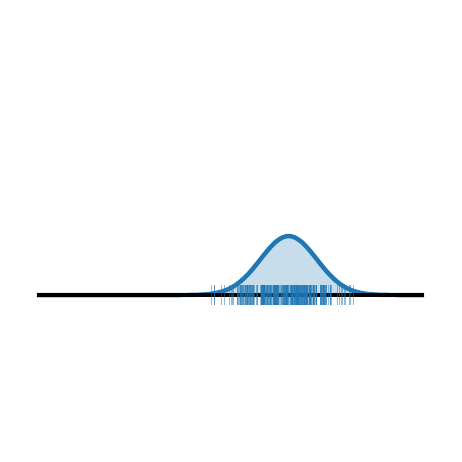
\begin{tikzpicture}
\begin{axis}[axis lines={none}, height={6.5cm}, width={6.5cm}, xmin={-3}, xmax={3}, ymin={-3}, ymax={3}, clip mode={individual}]
    \node at (-3,-3) {};
    \node at (-3,3) {};
    \node at (3,3) {};
    \node at (3,-3) {};
    \addplot[no markers, smooth, ultra thick, color={rgb,1:red,0.1216;green,0.4667;blue,0.7059}, fill={rgb,1:red,0.1216;green,0.4667;blue,0.7059}, fill opacity={0.25}]
        coordinates {
            (-3.0,-1.0)
            (-2.9,-1.0)
            (-2.8,-0.9999999999999998)
            (-2.7,-0.9999999999999986)
            (-2.6,-0.9999999999999909)
            (-2.5,-0.9999999999999438)
            (-2.4,-0.9999999999996723)
            (-2.3,-0.9999999999981868)
            (-2.2,-0.999999999990484)
            (-2.1,-0.9999999999526182)
            (-2.0,-0.9999999997761739)
            (-1.9,-0.9999999989968812)
            (-1.8,-0.9999999957348286)
            (-1.7,-0.99999998279467)
            (-1.6,-0.9999999341536179)
            (-1.5,-0.9999997609200129)
            (-1.4,-0.9999991764368138)
            (-1.3,-0.9999973085084408)
            (-1.2,-0.9999916549005841)
            (-1.1,-0.9999754522097821)
            (-1.0,-0.9999314928836516)
            (-0.9,-0.9998186150009755)
            (-0.8,-0.9995443730100476)
            (-0.7,-0.9989141748075886)
            (-0.6,-0.9975449927421185)
            (-0.5,-0.99473391284028)
            (-0.4,-0.9892831858053971)
            (-0.3,-0.9793087963610623)
            (-0.2,-0.9620992150531535)
            (-0.1,-0.9341352496846472)
            (0.0,-0.8914073851657249)
            (0.1,-0.8301404663464845)
            (0.2,-0.7479295366289559)
            (0.3,-0.6451078543883948)
            (0.4,-0.5259619407034923)
            (0.5,-0.3992795303462793)
            (0.6,-0.2777724583187935)
            (0.7,-0.17620707699520421)
            (0.8,-0.1085346586964997)
            (0.9,-0.08476363969709866)
            (1.0,-0.1085346586964997)
            (1.1,-0.17620707699520421)
            (1.2,-0.2777724583187935)
            (1.3,-0.3992795303462793)
            (1.4,-0.5259619407034923)
            (1.5,-0.6451078543883946)
            (1.6,-0.747929536628956)
            (1.7,-0.8301404663464844)
            (1.8,-0.8914073851657249)
            (1.9,-0.9341352496846472)
            (2.0,-0.9620992150531535)
            (2.1,-0.9793087963610624)
            (2.2,-0.9892831858053971)
            (2.3,-0.99473391284028)
            (2.4,-0.9975449927421185)
            (2.5,-0.9989141748075886)
            (2.6,-0.9995443730100476)
            (2.7,-0.9998186150009755)
            (2.8,-0.9999314928836516)
            (2.9,-0.9999754522097821)
            (3.0,-0.9999916549005841)
        }
        ;
    \draw[black, ultra thick] ({rel axis cs:1,0}|-{axis cs:0,-1}) -- ({rel axis cs:0,0}|-{axis cs:0,-1});
    \addplot[only marks, mark={|}, mark size={3.5pt}, color={rgb,1:red,0.1216;green,0.4667;blue,0.7059}, opacity={0.5}]
        coordinates {
            (1.029584828171896,-1)
            (1.0666825380016693,-1)
            (0.6394971710765831,-1)
            (0.895447023418512,-1)
            (0.5342766730802563,-1)
            (1.0356102884703913,-1)
            (1.9004055890657514,-1)
            (-0.0882000290702114,-1)
            (1.1310066390066154,-1)
            (1.0880522835745536,-1)
            (1.1544325438019485,-1)
            (1.3198803581543697,-1)
            (1.0999823409289662,-1)
            (0.6723186859902927,-1)
            (1.078015618822017,-1)
            (0.8780088187141819,-1)
            (0.5976433864840105,-1)
            (0.12680401057023116,-1)
            (0.9526406636981474,-1)
            (0.5697554152288482,-1)
            (0.1460167608353189,-1)
            (1.2469459607568574,-1)
            (1.192073246220382,-1)
            (1.1401109846334934,-1)
            (0.8723756556011468,-1)
            (1.4827598481127873,-1)
            (0.8681152499422684,-1)
            (0.5750596377747341,-1)
            (0.36819029891689237,-1)
            (0.8768205359630236,-1)
            (0.8280187304433074,-1)
            (-0.02206851410671773,-1)
            (0.8708965094154091,-1)
            (1.4328587659806213,-1)
            (1.1474527139706738,-1)
            (1.232801467206325,-1)
            (1.065027425741845,-1)
            (0.6185907671873769,-1)
            (0.6102874187495657,-1)
            (0.11407904602211116,-1)
            (0.33811717614057146,-1)
            (0.7538591604587681,-1)
            (0.9307161153126997,-1)
            (1.0489844491540699,-1)
            (1.6563411788632494,-1)
            (1.4666202323523352,-1)
            (0.9899520176410608,-1)
            (0.46024814056266505,-1)
            (0.5294693236711454,-1)
            (1.3922981596901058,-1)
            (0.3121878941168523,-1)
            (1.4406302695563338,-1)
            (0.8757439944207485,-1)
            (1.231010520130199,-1)
            (0.8868069699771162,-1)
            (0.7426077140987116,-1)
            (0.025036819111500463,-1)
            (0.6520400550785271,-1)
            (0.3988889798440649,-1)
            (1.7197442010199036,-1)
            (0.2589696240201562,-1)
            (0.6667069467573212,-1)
            (0.4800009251461627,-1)
            (0.2962453907117797,-1)
            (0.9585401163623082,-1)
            (0.6314409715436357,-1)
            (0.1502740211836675,-1)
            (1.0398200875657426,-1)
            (0.2691047804514879,-1)
            (0.6854239638388055,-1)
            (0.7199393838365724,-1)
            (1.3367305134447531,-1)
            (1.4120317190789868,-1)
            (0.32158703647992415,-1)
            (0.20553373948494247,-1)
            (0.7087707550144227,-1)
            (1.4343127419017703,-1)
            (1.549079403991433,-1)
            (1.8412751037900579,-1)
            (0.5035672869103921,-1)
            (1.4003232695714372,-1)
            (0.679844133616686,-1)
            (0.7835881782333155,-1)
            (1.5534348663185078,-1)
            (1.2475368261469093,-1)
            (0.8251836652999842,-1)
            (0.6955329383839233,-1)
            (0.9948601116135241,-1)
            (1.056548289667431,-1)
            (1.0394955395206757,-1)
            (1.0129897778510424,-1)
            (1.1003768343547842,-1)
            (0.9915309322945648,-1)
            (1.563936760342973,-1)
            (1.4491317366763443,-1)
            (0.8279547665167923,-1)
            (0.9680836018752585,-1)
            (0.5450481923632396,-1)
            (0.15468572832528016,-1)
            (1.5538077623570097,-1)
            (0.843806975940564,-1)
            (0.7037693561968855,-1)
            (0.22579526442898146,-1)
            (0.042715354726225785,-1)
            (1.521179815429401,-1)
            (0.7262457872234388,-1)
            (1.2772012581302006,-1)
            (0.23531724469722226,-1)
            (0.891964442492118,-1)
            (0.625474450859717,-1)
            (1.0741116005386968,-1)
            (0.7489081472103332,-1)
            (0.9574252730070444,-1)
            (1.4611405367158943,-1)
            (1.1751734805246028,-1)
            (0.36223124142358565,-1)
            (0.5257516916655526,-1)
            (1.0125755734721347,-1)
            (0.26360542041860835,-1)
            (1.1220978596908742,-1)
            (0.3569244686913795,-1)
            (0.3195456983078354,-1)
            (0.30687023786814094,-1)
            (1.1366549785422686,-1)
            (-0.2481312390134759,-1)
            (0.9653405231285416,-1)
            (0.17695631837263337,-1)
            (-0.29808721961121665,-1)
            (0.7177691580794013,-1)
            (0.2760993725755183,-1)
            (1.4030429898771897,-1)
            (0.6883630388734756,-1)
            (1.2380056079362312,-1)
            (1.2295587557354748,-1)
            (0.19092514418374695,-1)
            (0.48822161010372356,-1)
            (1.1869561995391498,-1)
            (0.7043066939158933,-1)
            (1.4165807111088022,-1)
            (1.7594094203903865,-1)
            (0.8677356654885773,-1)
            (0.8118969424595366,-1)
            (0.2644714727718115,-1)
            (1.6834432155141692,-1)
            (0.5048716362737153,-1)
            (0.4770907531441041,-1)
            (0.5648317086366266,-1)
            (0.727390516232979,-1)
            (1.107127308546585,-1)
            (1.1783733791119275,-1)
            (0.7261898840547666,-1)
            (0.8649777095528668,-1)
            (1.3366919062210385,-1)
            (0.5927653356175736,-1)
            (0.27491185890728176,-1)
            (1.08950354460642,-1)
            (0.8598084342308725,-1)
            (0.6977109573574093,-1)
            (1.8536540167470752,-1)
            (1.1524418909054648,-1)
            (0.5012809340647827,-1)
            (0.8324109779304253,-1)
            (0.9264662842813131,-1)
            (0.7819353515586007,-1)
            (0.9484024771992164,-1)
            (1.1801881360597786,-1)
            (0.42344328503681855,-1)
            (0.9378170852107978,-1)
            (0.8691481890087134,-1)
            (1.4447359220165579,-1)
            (0.965908027958606,-1)
            (1.0548097178246478,-1)
            (0.4966521206561851,-1)
            (0.798392615055012,-1)
            (1.4930765785177207,-1)
            (1.2187215459441192,-1)
            (1.1086769258936393,-1)
            (1.1637719599908158,-1)
            (1.4566194568750752,-1)
            (0.291410852454145,-1)
            (0.951042635453708,-1)
            (1.1731654556809934,-1)
            (1.0366002056792936,-1)
            (1.3298974013892617,-1)
            (1.1208255516868904,-1)
            (1.2800155926316923,-1)
            (1.2049331134228005,-1)
            (1.7759883898566633,-1)
            (0.9665598121571971,-1)
            (0.5565615076832997,-1)
            (1.335313310800165,-1)
            (0.6840644292313198,-1)
            (1.0585936645899205,-1)
            (1.1943757732922569,-1)
            (1.1619218661721789,-1)
            (0.24523372753310224,-1)
            (0.7375283009466356,-1)
            (0.34352521313924667,-1)
            (1.1811949261518027,-1)
            (1.7307557908577134,-1)
            (0.2077507002609158,-1)
            (1.029626663680191,-1)
            (1.0320233874164235,-1)
            (0.8556398765539684,-1)
            (0.6247015815448483,-1)
            (1.1719346420528685,-1)
            (0.01844258630818485,-1)
            (0.5838409446219854,-1)
            (0.47645616170586136,-1)
            (0.10761037664853879,-1)
            (1.280056399159755,-1)
            (0.16749061782694707,-1)
            (0.6653827431074919,-1)
            (0.42420190637933575,-1)
            (-0.13443506769569835,-1)
            (1.4750850616945534,-1)
            (1.0276542168944816,-1)
            (1.1910438043996137,-1)
            (0.9920254894201074,-1)
            (1.0418622004665874,-1)
            (1.0369856223548666,-1)
            (0.35792168661652013,-1)
            (1.2802892099678544,-1)
            (1.0753732878330338,-1)
            (0.4996771726988574,-1)
            (1.1462748371106515,-1)
            (0.5187964210290879,-1)
            (0.68771313571544,-1)
            (0.6695198243283164,-1)
            (1.180840822782021,-1)
            (1.2966269018756036,-1)
            (0.3059561428580503,-1)
            (1.2809614944840755,-1)
            (0.5273606248024915,-1)
            (1.229139404178201,-1)
            (0.5322752171103267,-1)
            (1.0210304992682624,-1)
            (0.506375866532563,-1)
            (0.24034562361380685,-1)
            (0.6125846816098957,-1)
            (0.5772899789960086,-1)
            (1.3948016807968122,-1)
            (0.5095542463197718,-1)
            (0.9093149534289493,-1)
            (0.22243557334542474,-1)
            (0.9844475342897381,-1)
            (1.3012998862357688,-1)
            (0.9713311815901338,-1)
            (1.0136187936640892,-1)
            (-0.24227747499702235,-1)
        }
        ;
\end{axis}
\end{tikzpicture}
\end{document}

\caption{Sample from conditional distribution.}
\end{subfigure}
\caption{Illustration of distributional conditioning of a bivariate Gaussian. Here, we form the joint distribution, calculate the conditional distribution, and then draw samples from it. Note that all steps except the very last one are \emph{distributional} in nature and do not involve the use of random variables, which only appear at the very end of the process.}
\label{fig:dist-cond-mvn}
\end{figure*}

The non-singularity requirement is more-or-less necessary: otherwise, the marginal distribution of $\v{y}$ may admit too many null sets, rendering the desired conditional distribution non-unique, except in regions where one can apply a linear map to recover a suitable Lebesgue density and apply the above argument on the obtained subspace.

Of one wants to work with this expression numerically, then it's possible to calculate the desired conditional mean and covariance. 
In particular, one can generate conditional sample via the expression
\[
(\v\theta\given\v{y})(\omega,\v\gamma) &= \m{L}_{\v\theta\given\v{y}}\v{z}(\omega) + \v\mu_{\v\theta\given\v{y}}
&
\v{z} &\~[N](\v{0},\m{I})
\]
where $\v\mu_{\v\theta\given\v{y}}$ is the conditional mean, and $\m{L}_{\v\theta\given\v{y}}$ is a Cholesky factor of the conditional covariance.
This enables one to calculate any quantity of interest depending on the conditional distribution numerically via the Monte Carlo method.
The computational costs will be cubic in the dimension of both $\v\theta$ and $\v{y}$, owing to the need to compute $\m{L}_{\v\theta\given\v{y}}$ and invert $\m\Sigma_{\v{y}\v{y}}$, respectively.


\subsection{Pathwise conditioning}

The preceding considerations gave us closed-form analytic expressions for Gaussian conditionals in terms of matrix-vector expressions that can be computed numerically.
From this, one might be tempted to conclude that there is nothing more to say conditioning multivariate Gaussians---this, however, would be a significant mistake.
Miraculously, Gaussian conditional distributions---in general, a purely \emph{distributional} notion---can also be described in a \emph{pathwise} manner using \emph{random variables}.

\begin{restatable}[Matheron's update rule]{theorem}{thmmvnpw}
\label{thm:mvn-pw}
For $\v\theta,\v{y}$ defined in \Cref{prop:mvn-cond}, we have that
\[
(\v\theta\given\v{y})(\omega,\v\gamma) = \v\theta(\omega) + \m\Sigma_{\v\theta\v{y}}\m\Sigma_{\v{y}\v{y}}^{-1}(\v\gamma - \v{y}(\omega))
.    
\]
\end{restatable}

\begin{proof}
By direct calculation,
\[
\E(\v\theta + \m\Sigma_{\v\theta\v{y}}\m\Sigma_{\v{y}\v{y}}^{-1}(\v\gamma - \v{y})) = \v\mu_{\v\theta} + \m\Sigma_{\v\theta\v{y}}\m\Sigma_{\v{y}\v{y}}^{-1}(\v\gamma - \v\mu_{\v{y}}) = \E(\v\theta\given\v{y}=\v\gamma)
\]
and 
\[
\Cov(\v\theta + \m\Sigma_{\v\theta\v{y}}\m\Sigma_{\v{y}\v{y}}^{-1}(\v\gamma - \v{y})) &= \m\Sigma_{\v\theta\v\theta} + \m\Sigma_{\v\theta\v{y}}\m\Sigma_{\v{y}\v{y}}^{-1}  \m\Sigma_{\v{y}\v\theta} - 2\m\Sigma_{\v\theta\v{y}}\m\Sigma_{\v{y}\v{y}}^{-1} \m\Sigma_{\v{y}\v\theta}
\\
&= \m\Sigma_{\v\theta\v\theta} - \m\Sigma_{\v\theta\v{y}}\m\Sigma_{\v{y}\v{y}}^{-1}  \m\Sigma_{\v{y}\v\theta} = \Cov(\v\theta\given\v{y}=\v\gamma)
\]
where we have cancelled a factor of $\m\Sigma_{\v{y}\v{y}}\m\Sigma_{\v{y}\v{y}}^{-1}$ in the middle term.
\end{proof}

This affirms the claim, but gives few hints on where this expression originates or how to obtain it from first principles.
To better understand this, we now prove \Cref{thm:mvn-pw} in a different way.
To do so, we first prove a general result about conditioning.

\begin{lemma}
\label{lem:cond-repr}
Consider three random vectors $\v{a} : \Omega \-> \R^m$, $\v{b} : \Omega \-> \R^n$, and $\v{c} : \Omega \-> \R^m$ such that 
\[
\v{a} = f(\v{b}) + \v{c}    
\]
where $f : \R^n \-> \R^m$ is a measurable function, and where the random variables $\v{b}$ and $\v{c}$ are independent. 
Then we have 
\[
(\v{a} \given \v{b} = \v\beta) = f(\v\beta) + \v{c}    
.
\]
\end{lemma}

\begin{proof}
This follows by direct calculation by writing
\[
\int_{A_{\v{b}}} \pi_{\v{a}\given\v{b}}(A_{\v{a}}\given\v\beta) \d\pi_{\v{b}}(\v\beta) &= \P(\v{a} \in A_{\v{a}}, \v{b} \in A_{\v{b}}) 
\\
&= \P(f(\v{b}) + \v{c} \in A_{\v{a}}, \v{b} \in A_{\v{b}})
\\
&= \int_{\R^m\x\R^n} \1_{f(\v\beta) + \v\varsigma \in A_{\v{b}}, \v\beta\in A_{\v{b}}} \d(\pi_{\v{c}}\ox\pi_{\v{b}})(\v\varsigma,\v\beta)
\\
&= \int_{A_{\v{b}}} \int_{\R^m} \1_{f(\v\beta) + \v\varsigma \in A_{\v{b}}} \d\pi_{\v{c}}(\v\varsigma) \d\pi_{\v{b}}(\v\beta)
\\
&= \int_{A_{\v{b}}} \P(f(\v\beta) + \v{c} \in A_a) \d\pi_{\v{b}}(\v\beta)
\]
where we have used independence to represent the probability as an integral over a product measure, followed by Tonelli's Theorem.
By the Disintegration Theorem, $\pi_{\v{a}\given\v{b}}$ is $\pi_{\v{b}}\ae[-]$ unique, implying that the conditional distributions of interest are equal, and the claim follows.
\end{proof}

The key idea behind our argument will be to choose the \emph{conditional expectation} for our function $f$, or more precisely, the map $\v{y} \|> \E(\v\theta\given\v{y})$.
We now recall this notion and some of its key properties.

Conditional expectation is defined as the orthogonal projection from the Lebesgue space $L^2(\Omega,\c{F},\P;\R^n)$ onto the subspace $L^2(\Omega,\sigma(\v{y}),\P;\R^n)$ where $\sigma(\v{y})$ is the smallest $\sigma$-algebra containing all preimages $\v{y}^{-1}(A_{\v{y}})$ where $A_{\v{y}}\in\c{B}(\R^n)$. 
Recall that the preimage is a map $\v{y}^{-1} : \c{B}(\R^n) \-> \c{F}$ between $\sigma$-algebras.
This definition might seem daunting, but is reasonably intuitive: we can think of this as projecting onto the subspace induced by all collections of random numbers in $\Omega$ which play a role in determining what $\v{y}$ does.

Recall that $L^2(\Omega,\c{F},\P;\R^n)$ is a Hilbert space of equivalence classes of random variables with inner product given by $\innerprod{\v{a}}{\v{b}} = \E(\v{a}\cdot\v{b})$.
Using this, it follows from the Projection Theorem for Hilbert spaces that the terms\footnote{TODO: check.} $\E(\v\theta\given\v{y})$ and $(\v\theta - \E(\v\theta\given\v{y}))$ are uncorrelated---and, in the Gaussian case, that they are independent.
This gives us the candidate random variables to use for $\v{b}$ and $\v{c}$, if we choose conditional expectation for $f$.

Finally, recall that for multivariate Gaussians, we have $\E(\v\theta\given\v{y}) = \m\Sigma_{\v\theta\v{y}}\m\Sigma_{\v{y}\v{y}}^{-1}\v{y}$, where we note in our setting that the inverse always exists by non-singularity of $\v{y}$.
With these preparations, we are ready to revisit \Cref{thm:mvn-pw}.

\thmmvnpw*

\begin{proof}
Write 
\[
\v\theta = \E(\v\theta\given\v{y}) + (\v\theta - \E(\v\theta\given\v{y}))
\]
and note that since $\E(\v\theta\given\v{y})$ and $(\v\theta - \E(\v\theta\given\v{y}))$ are uncorrelated and jointly Gaussian, they are independent.
Applying \Cref{lem:cond-repr} yields
\[
(\v\theta\given\v{y}=\v\gamma) &= \m\Sigma_{\v\theta\v{y}}\m\Sigma^{-1}_{\v{y}\v{y}} \v\gamma + (\v\theta - \m\Sigma_{\v\theta\v{y}}\m\Sigma^{-1}_{\v{y}\v{y}} \v{y})
\\
&= \v\theta + \m\Sigma_{\v\theta\v{y}}\m\Sigma^{-1}_{\v{y}\v{y}}(\v\gamma - \v{y})
\]
where we have substituted $\E(\v\theta\given\v{y}) = \m\Sigma_{\v\theta\v{y}}\m\Sigma^{-1}_{\v{y}\v{y}} \v{y}$. 
The claim follows.
\end{proof}

\begin{figure*}[t]
\begin{subfigure}{8cm}
\documentclass[tikz,11pt]{standalone}
\usepackage{lmodern}
\usepackage{pgfplots}
\pgfplotsset{compat=1.17}
\usepgfplotslibrary{external}
\usepgfplotslibrary{groupplots}
\usepgfplotslibrary{fillbetween}
\usetikzlibrary{fadings}
\begin{document}
\tikzsetnextfilename{figures/tex/mvn-pw-joint.pdf}
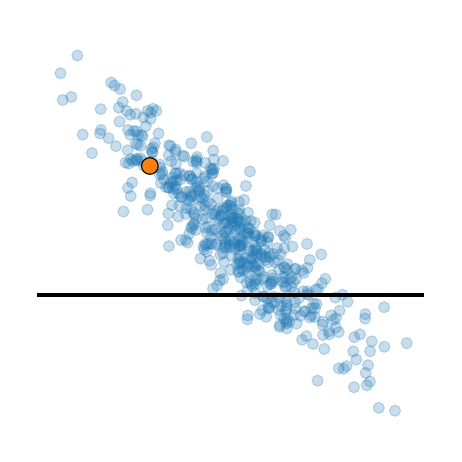
\begin{tikzpicture}
\begin{axis}[axis lines={none}, height={6.5cm}, width={6.5cm}, xmin={-3}, xmax={3}, ymin={-3}, ymax={3}, clip mode={individual}]
    \node at (-3,-3) {};
    \node at (-3,3) {};
    \node at (3,3) {};
    \node at (3,-3) {};
    \addplot[only marks, color={rgb,1:red,0.1216;green,0.4667;blue,0.7059}, opacity={0.25}]
        coordinates {
            (0.2972879845354616,-0.10087664808024613)
            (-0.5976344767282311,0.5333180524739201)
            (-0.839026854388764,0.8907344574202789)
            (2.2950878238373105,-3.053779070523791)
            (0.5299655761667461,-0.28891673497551795)
            (0.5837082875687786,-0.105457100657531)
            (0.45879095505371686,-0.6405931735580526)
            (0.40839583832475224,-0.38954743577809514)
            (-0.6936536438038856,-0.1489077100062718)
            (0.12076596493743928,-0.43893395321484724)
            (-1.7297561813906863,1.903726524008475)
            (0.6700619812560624,-0.3629447984969627)
            (-0.06337459242956062,0.6397969812993919)
            (-0.07314863333773934,-0.25910659222130056)
            (-1.2200551285346526,1.074870151644211)
            (-0.1651363578028337,-0.7734457920841674)
            (-0.0667679865065892,0.5929499538365516)
            (0.5676954597384435,-0.1781244465582743)
            (0.37859887985335006,-0.6221482246806381)
            (-0.6646462443910314,-0.18773933402596066)
            (-1.2890476038497443,1.0140020039235378)
            (0.07046760136115796,0.08556360792902756)
            (1.7351656660543822,-0.9950288670966089)
            (0.20636408140261675,-0.62547953269969)
            (-0.8500556703153979,1.257348262973964)
            (-1.348533456491827,1.754310380398978)
            (-0.055647093207324264,0.38109290401679086)
            (-0.030266886646762546,-0.13015208791920213)
            (-2.0073032025325626,1.5586129373578335)
            (-1.1496275243969976,1.8544089729772013)
            (-1.4706245413873802,1.0902690340059635)
            (-0.9635439598255011,0.26343495455473065)
            (0.13430023756127,-0.3894292422615074)
            (-1.719989356319742,1.6878105082535104)
            (-1.4473728978815112,1.0880595719321655)
            (-0.4130873839831828,0.8085091590296176)
            (1.174681325975111,-1.6356261568976758)
            (-1.593214868044067,1.2426641362540831)
            (1.225797497997867,-0.4541383442066472)
            (2.1594331871008534,-2.3399225814803764)
            (1.1478203006125018,-1.2531941369345656)
            (-0.2670670352181297,0.8937951980148244)
            (0.7973041601753904,-0.792390078857867)
            (-0.46907960993009634,0.5170317605506107)
            (0.35914640760234967,-0.18373622732143902)
            (0.2592163280556861,-0.032917860895333384)
            (0.20998636004214272,0.4749490363050444)
            (1.2597946036121963,-1.2058603767341844)
            (0.15619449488763584,-0.4955268530356326)
            (-1.7098682060045913,2.192689147761142)
            (-0.1289156385300165,-0.08020656912609962)
            (-1.546731741900333,0.5347739224365254)
            (1.4250842322231618,-1.456330021777407)
            (0.865359034508392,-1.4435058863603305)
            (-0.018434833227298542,-0.2579341992357144)
            (0.3994394061296323,-0.5105873183063359)
            (0.13174261149628444,0.44257218636923823)
            (0.6312912597626849,-1.1059308923628306)
            (-0.8585845030636355,0.8853016262294067)
            (-1.4599892950591262,1.5360882252440877)
            (-1.2459007156231243,0.5408563423686472)
            (-1.360732996599522,1.4613146754818385)
            (-2.63399370777994,2.4359348601304873)
            (-1.6587759684101517,0.29481115195791996)
            (-0.4180662233306449,-0.24764102642690128)
            (1.1540597669111703,-1.2502907513465775)
            (0.7754380459705584,-0.36833548563802787)
            (-1.626729284162485,1.0522779658499601)
            (0.658322671059814,-0.7881837100379394)
            (1.1851174294240252,-0.2071962660912362)
            (-0.0740194597978335,-0.021485543722413278)
            (-1.458002434697322,2.0956454067417587)
            (-0.9064866353733989,0.39292872498016307)
            (-0.7689287953327062,0.5194264320324146)
            (0.4751826349484905,-0.14929099234171395)
            (-0.3987477530370317,0.32385068728619537)
            (1.0018399414103412,-1.2088906116517335)
            (-1.4340505462257125,1.4801490362095613)
            (-0.09220577556331351,-0.11930384463560857)
            (2.187832361106393,-1.7166072340902891)
            (-0.9147242711971281,0.7556628220078405)
            (0.060717820312243403,-0.17271068672241838)
            (0.11104289827811374,0.18024952760947624)
            (-1.0932960849422242,1.0217835616587996)
            (-0.07077890859801883,0.6084369397547749)
            (0.1512033860208509,0.018726670405881995)
            (-0.9253434974479612,0.731201762758177)
            (1.3606109850208474,-0.9058283405746437)
            (0.4787377009574211,-0.1670919708708632)
            (1.276972611856289,-1.7578644982165152)
            (0.11709983671299977,0.1677756026392937)
            (0.3133823643278484,0.14785327349419808)
            (0.5066085599761962,-0.07593211134688438)
            (0.6995645399732705,0.24638030388071974)
            (0.15269868152330113,-0.4808673056876713)
            (0.9986772266084378,-1.1147450747162742)
            (0.3638388194911837,-0.033079164249808446)
            (0.6008899714463747,-1.195567246768635)
            (-0.3727356407152467,-0.22101271021703134)
            (0.6451054034379425,0.250160927763565)
            (-1.5881288112102452,1.5589425937694117)
            (0.3028824231221631,-0.3169543042559784)
            (-0.6315778870329364,0.8403547403825111)
            (-2.0224314101114222,1.5040292137222653)
            (-0.9716762048860438,0.08211896104597816)
            (0.8719091772543835,-1.5172276417019983)
            (-0.5382489016869288,0.008625917897571722)
            (-2.373156801968529,2.7109261834662295)
            (0.2928588585051935,0.02747083174493936)
            (0.21112095190111557,-0.04814665624441669)
            (0.3142665708225735,-0.824918227123796)
            (0.8724432818783148,-0.6098256658574496)
            (-0.918403552104298,1.0728380340045198)
            (-0.8745409882369648,0.5748000251287083)
            (-0.5287577864433531,0.756722830581039)
            (0.909924517665989,-1.41297592304134)
            (0.8739856083349014,-1.1592264226989197)
            (0.7550975795526141,-1.047312604487026)
            (0.27766300810348893,-0.6435208407605771)
            (-1.513350928595663,1.0746005173459925)
            (-0.7403475629601508,1.161114487460948)
            (-0.8957439911719416,0.8154845454836968)
            (-1.5544394018554584,1.4834429959596507)
            (0.9206450790295183,-0.7572493895364327)
            (0.2606593892993496,-1.376870925366437)
            (-1.0562153109753674,0.9112105616016073)
            (0.27865272355818926,-0.27954244300337383)
            (-0.1569479584427068,-0.6603783867108125)
            (-0.5674519382746356,0.11002863000303026)
            (-3.8819978594268876,3.8715166318421317)
            (0.432306709021104,-0.5298667000323366)
            (0.3402161710448687,-0.4367949598488905)
            (1.9136035721789713,-2.42799190804498)
            (0.5169712744781768,-1.0243382924896245)
            (1.0840840119878734,-1.3219551464549286)
            (-0.025668064894330093,0.018104867554613876)
            (1.4678868411216563,-0.7475344564343945)
            (0.27236940715678176,-0.052305515584656515)
            (-1.1966483101519632,1.2882069773574079)
            (1.4147590837932418,-0.8177050497305656)
            (-0.1978660512585745,0.32145282082298665)
            (-1.7983067508193347,2.2463755315612124)
            (-0.5232908450257276,0.6605313698453924)
            (0.07774415899993356,-0.007529835312156244)
            (-0.43422769970595093,0.49710846972113587)
            (-0.12389276233418343,0.2984527837168319)
            (1.189248289168407,-0.9805534479118881)
            (1.0218854109275881,-1.4423571264238406)
            (2.3805130457880845,-1.188033443784486)
            (2.1299921566412503,-2.085970102894445)
            (-0.23211025519653547,0.29881002254612327)
            (1.107610369079468,-0.6190411563111236)
            (1.6776251628069427,-2.133117254191005)
            (-1.3830239105437792,1.477600144441786)
            (0.27246958339005234,0.27523273174208196)
            (0.6546787209966946,-0.7421339359792656)
            (-3.2998673372242706,2.4329415466777466)
            (0.5439858444482804,-0.455308019368296)
            (-1.8487276149711611,2.2922382967671315)
            (-0.10777043967832316,-0.26447033241910123)
            (-2.1473888794968143,1.1989359932661814)
            (-1.3931348022399552,1.1196084377040847)
            (0.8249874857828697,-0.07914426711418421)
            (-0.7164282891787297,0.8537985786816389)
            (-1.4667181528682052,1.8082132347320654)
            (0.8156139596767987,-0.7310011388445395)
            (-0.5908786155028164,0.8010190136191977)
            (-1.0802915526773837,0.7334208710621327)
            (-0.5775086066033142,1.0660012496529352)
            (0.6635670227160482,-1.026025748737541)
            (0.3786665366937789,-0.5634799820300157)
            (0.2624053715987166,-0.9380903867743564)
            (-1.774970345560557,1.306970598477777)
            (1.9168347916309745,-1.6512853829357856)
            (-0.7629697960098806,0.519096125677645)
            (-0.19755430324781426,0.6564511543726108)
            (0.15137376741018294,-0.14590883137280247)
            (0.8448917445918529,-0.7125551091022019)
            (-0.5595352207192429,0.24226993625911364)
            (1.633608902780053,-1.3568888711086873)
            (0.9401341655808859,-0.8759797406628419)
            (-0.001285241025904152,-0.16681927145477513)
            (0.04414459834517204,0.1977061652106734)
            (-0.36690604870636645,-0.03950040691101725)
            (0.7209794667689048,-0.2720741629778893)
            (0.3536205284606749,-0.5494390717986374)
            (-0.5293369148430024,1.069815877530889)
            (-0.7940239797611804,0.38289998576785605)
            (-0.9540680773126435,-0.24139761982770558)
            (-0.11409699214027211,-0.7515973911431816)
            (-0.393771885226301,1.0479161238455657)
            (0.26835044888970766,-1.3153914225138363)
            (1.5310536307073936,-1.6059775212726701)
            (0.5834052352999808,-0.4940769489651093)
            (-0.6101715120745413,1.3519805785953578)
            (-0.2805179483106536,0.2579073363572935)
            (0.131810280826272,0.32274053423714155)
            (-0.17667143438293495,0.18265907962212377)
            (0.8325802393139106,-0.2751839789726437)
            (-0.5993789779066115,0.027342200479943735)
            (0.16820569915460176,-1.0085515999241068)
            (0.13120625565482671,0.11975436757503295)
            (0.8698862875353852,-1.1016873222639396)
            (-0.029032421388993576,0.3927881400528105)
            (-0.15393921542968417,0.22461126696996186)
            (0.08721657095184755,0.017521334567634453)
            (-0.06667541333469505,0.34542461644404543)
            (1.4334553034866289,-1.618302733519816)
            (-0.11640702062324493,1.079978295913763)
            (-0.24234887761151688,0.24857525734027514)
            (0.7338834687716466,-0.45848686850115805)
            (-0.3537417603088734,0.6117848490154096)
            (-0.3673488735340369,1.4499001176426503)
            (2.3829332688009828,-1.8011477753527503)
            (0.03131929472379513,0.1487019051192954)
            (-0.9579189021380435,1.1655608420359491)
            (0.6274414959863405,-0.826801156755987)
            (-0.29438920541698516,-0.200918090551567)
            (-1.590717875491105,0.6580481529553509)
            (-1.2289146699114444,1.2627103366824262)
            (0.3914757161202707,-0.8272802027459634)
            (1.6896534499381899,-1.241659010120253)
            (-0.611968992291528,0.793946425577545)
            (0.3740840174093429,0.12267077653416325)
            (0.5808485859606817,-1.1829178552331354)
            (-1.5457001328588873,1.1048227019238768)
            (1.75361653512699,-2.141628353274176)
            (-0.531704625724874,0.1922036314355785)
            (-1.4980375731640485,1.5411885401438887)
            (0.5852478579163195,-0.10032099522446003)
            (-0.6877739300923975,0.59851727586995)
            (0.9966182023827315,-0.5954799621209282)
            (0.9599688052642058,-0.24886990064144054)
            (-0.40406029223492207,0.5491396778484607)
            (2.297379718927148,-2.747884960531122)
            (-1.3942524420044087,1.3121107080076224)
            (1.30993212700943,-1.2054498085495136)
            (0.746144255590275,-1.2261354102499837)
            (1.9487894951751723,-1.9989987359284322)
            (-0.6132329004972873,0.5591516786366368)
            (2.084230975839466,-1.3644751544267126)
            (0.38407455255519346,-0.3575657703398731)
            (-1.5785427534891785,1.0368323514483362)
            (1.8128382404129062,-1.1032328963834872)
            (-1.2123395817818958,1.2143991979887445)
            (0.2083343858982014,0.11785096365280404)
            (1.4046974354664667,-0.3700884195731384)
            (0.34013510486070253,-0.8585151885806933)
            (-1.2390463290112987,1.7286347285810262)
            (-0.8565863624820894,0.6856724400310634)
            (0.4538012969765639,-1.2950391361408786)
            (-0.9991007427732405,0.6724692092684246)
            (0.4662463238027101,-0.11655524693662578)
            (-0.792486173126059,0.8889859149331651)
            (0.1422610288642994,0.04166996146333768)
            (0.5165798439917115,-0.7175689095522795)
            (0.572932361603122,-1.0565363708688371)
            (0.1566513785833087,-0.7260310725566597)
            (0.23826183544768417,-0.43088636042927625)
            (1.193523304759714,-0.9433041331298971)
            (0.4091271950968771,-0.7560125520346963)
            (-0.32605180937465755,-0.4666031522072205)
            (-0.528112745560178,1.0969320628151762)
            (-1.0884645271492055,0.9753804876900225)
            (-0.8554296175519289,1.2188976352376453)
            (1.675948808787312,-1.574676993393196)
            (0.2666602308412965,-0.53143805527337)
            (-0.3688296792504201,0.20057296390434767)
            (0.06677792368156305,-0.2818814739091185)
            (-0.3523456900970411,0.44294736054753836)
            (-0.2405766371227846,-0.21836725104754706)
            (-0.3622644857512414,0.7616261111933353)
            (-1.2857410076345577,0.32351632878333625)
            (0.825156200939433,-0.8020049703309314)
            (1.7992548094594971,-2.1007188454222834)
            (0.10848097145565462,0.2719652356610049)
            (0.5949706804435368,-0.3489523943888211)
            (1.1079660978130559,-1.6929800308297969)
            (0.25989707779870364,-0.030648122518285303)
            (-0.3919576066101382,-0.2090688267826724)
            (-0.08111315760776971,-0.21741634978159619)
            (-0.630814741681354,0.8490910651791808)
            (1.13580872262362,-0.6569536540548457)
            (-0.0799246177593996,-0.18092074377431283)
            (-0.4387702731149963,0.17508014174444658)
            (0.0012495783650486236,-0.6069923524705545)
            (-0.4821758306182083,0.6013390644723547)
            (0.3126572456108897,-0.4289690059668188)
            (0.17824576718381163,-0.15713391453230402)
            (-0.03222208961967493,0.045146912348522014)
            (-1.525082270589168,0.7445062424975258)
            (-0.08789055046010402,-0.02513131951625694)
            (-1.3426658027254874,1.004408990932128)
            (-1.2401064426390593,0.5762565389382952)
            (0.1766983746369227,-0.6035758949232014)
            (0.8305441585121899,-1.3690803554375794)
            (-1.062426745485554,0.877465212758632)
            (-0.7792124017891849,0.7889399427741401)
            (-0.39607292077168643,0.8409048697721295)
            (-0.2687142882698926,1.2382128234154328)
            (-0.00119442020718918,0.3815958468627311)
            (1.3221375148350687,-0.9132684464335817)
            (-0.9611868737662628,0.6644334474884017)
            (0.9476400830565346,-0.7131257480218709)
            (0.4982972465694152,-1.0225669466212737)
            (0.1431480547985834,-0.29834175355580383)
            (-0.01653802057118619,-0.22275574923341357)
            (0.13323968501086753,-0.12938097895609246)
            (1.6326868249717172,-1.501554762860129)
            (0.009275324748154191,0.4261866431900248)
            (1.4319586745069863,-1.4102185712646864)
            (0.18314474353215668,-0.19438278991957553)
            (-1.612809018801593,1.8536949892686776)
            (1.29069196187616,-1.1368480152314493)
            (3.124318593443059,-3.2531886837614876)
            (-0.28715298455425015,0.9329817064205438)
            (-0.11556009086388684,-0.3507826440767556)
            (0.30077062196830734,0.914227110215188)
            (0.017529407674652085,0.4489838819899084)
            (-0.8089189600547338,0.21562178213204575)
            (-1.1710373555532807,1.351871086200737)
            (-0.7665852772824016,-0.14652733242349747)
            (0.11702518739433772,-0.6416873744306543)
            (1.0102928065517993,-0.5918397818918703)
            (1.9016982514072045,-1.8723224317422273)
            (-2.2895905972982606,1.4867380417532492)
            (2.5483208898247103,-2.791926964790314)
            (-1.365734006824005,1.0721329392212648)
            (-1.2367794349539312,1.8287278679932657)
            (0.7612395595485809,-1.4930083770916784)
            (1.5909826424480042,-1.3873394516726332)
            (0.8545444889487256,-1.2564957593207051)
            (-0.6367201621923837,0.45192057065970526)
            (0.988027300039114,-0.95824234844789)
            (0.3885790331353395,-0.08030636590725965)
            (-0.2614930295213064,1.099332727685738)
            (1.1932460546819013,-0.5769588061590163)
            (0.843689267655445,-1.062541317581636)
            (0.17404214583167332,-0.2227029745734701)
            (0.9331744539977493,0.010756726433466923)
            (0.15991438966878682,0.13971827764498546)
            (-0.11390296246278847,0.11219094460796383)
            (1.6254676981101484,-1.0382911566135475)
            (0.2628347548441931,-0.5627104759959763)
            (0.3513428690933362,-0.31512388586110723)
            (-0.6949663889620127,0.256576558860079)
            (-0.10884891545390497,0.7031555956921597)
            (2.729445820551839,-1.7458795930669253)
            (-0.36792522369791164,-0.3270176758895879)
            (-0.05528883473746865,0.13070422921872524)
            (-0.3339535425294759,-0.20661633831096599)
            (-0.5720644165807692,0.08638819724675634)
            (0.9822822445625023,-1.3098499689416847)
            (0.008154305444488837,0.17862785276080292)
            (0.37847076773415456,-1.0794003857716605)
            (-1.5531425959603435,1.793555441359969)
            (-1.2008763348459806,1.8861374274951346)
            (0.8379852615245372,-0.5713165764500935)
            (0.861525601405543,-0.8663091825668433)
            (-0.6624402142053086,0.4840225450502453)
            (2.094064358256568,-2.2054002029076734)
            (2.110576071498333,-2.397038788668987)
            (-0.21345648146548854,-0.2179959280815545)
            (0.6341198754901243,-0.7954371454868959)
            (0.6183000885232028,-0.8317625276625111)
            (-0.3091091627491842,0.9655192645873627)
            (-0.6815274819963835,0.346169784313342)
            (0.605999681311456,0.08051940055855189)
            (0.37619020514195034,-0.7971288514199739)
            (2.006165198118277,-1.6089884039003837)
            (-0.09982010028904506,-0.49023091987671963)
            (0.7638568575849538,-1.466578433623644)
            (0.3813870602943384,-0.9707439455834941)
            (-0.4088361702003478,-0.29326846874825335)
            (-0.520893143837836,0.6913758657094472)
            (-1.8898609632139673,1.4300757043367518)
            (0.30423375743841535,-0.46608275281434836)
            (0.8658098173642257,-1.2161642694291004)
            (0.31016224941683607,-0.7796798943093933)
            (0.782603001925965,-1.1693269362450032)
            (0.25032695818751377,-0.8058153926409749)
            (0.4707150121846368,-0.3534157937665088)
            (0.3923682520698269,-0.2638459560841252)
            (-2.0115667870090204,1.8811352161843016)
            (-0.8042222347395631,0.56886617179731)
            (-0.2895644050953529,0.8728501706922185)
            (-0.9560332307222564,0.6695465744839425)
            (-0.8694008603311896,0.7639064721703516)
            (0.8498592837097624,-0.11126015444974902)
            (-0.5184225058688992,1.1400616484531596)
            (0.6921663616623136,-0.4935800557806683)
            (0.6394740649295387,-0.6900115504415675)
            (0.55173629984778,-0.40789593571483923)
            (0.41052460590863105,-0.3193155693826418)
            (1.1274930637855678,-0.9403360898186511)
            (0.9746272376437478,-0.7977901419516686)
            (0.2718102677901078,0.03871248153621884)
            (0.5264904831050543,-0.4120638114084491)
            (-0.6085163875132199,0.054422712166160514)
            (0.3881780115667518,-0.07883848551640443)
            (-0.2535150437627753,0.9585987771793687)
            (0.6098239355865941,-0.4066558704215472)
            (-1.2821660632229595,1.8556326043232019)
            (-1.4507878031322263,1.1166069407343293)
            (0.12912659446021338,-0.24183971473231886)
            (-1.2132705181272156,1.2130290331673879)
            (-0.6417207530049402,-0.049623369119604965)
            (-0.39188919597096245,0.38111258647940705)
            (1.013630663300725,-0.7527935726315519)
            (-0.7156034341569465,1.146395116604524)
            (0.13277193762814965,-0.6343703576898402)
            (1.3084072697295053,-1.3399869816949301)
            (0.8817160139297816,-0.5229296348275051)
            (0.8462905517316545,-0.8813197451171236)
            (-0.5734932337841947,0.27931315180062166)
            (-0.20594816627575477,-0.8526678501707842)
            (-0.952539183118715,1.3209982076579012)
            (0.23745788510368965,0.6914320765870984)
            (0.8362686215120259,-0.5753258626258574)
            (-0.1973537715836528,0.49914054245865724)
            (0.47914911804336535,-0.3772305718350854)
            (-0.27097044634740913,-0.9013828933023016)
            (-0.4987134771226696,0.484510700795029)
            (0.06271981803961879,-0.2093436182957782)
            (0.14891084177869107,-0.2306471559660138)
            (0.13105150326944962,-0.5082799069312333)
            (-2.5991778979112783,2.0226988744915118)
            (2.1619447876295617,-1.8710714173102687)
            (-0.6169282510157554,0.3321726891751764)
            (1.5600696986005596,-1.3134412873715504)
            (1.0577653016664748,-1.0478741179021815)
            (1.3308298996034031,-1.136160788553338)
            (-0.08541243409544698,0.11578820322691277)
            (0.4798881756377317,-0.7542036412810156)
            (-0.6357559693783907,0.6051696574941969)
            (1.4528570085121595,-1.834090975630855)
            (-0.2017657745270218,0.14837003558261336)
            (-0.30420165880389033,0.4067494198257332)
            (-0.47935690712903745,0.6742048242630732)
            (-1.6704355359969572,1.9914560968495558)
            (-0.23832634399885072,0.016437442091930154)
            (2.0885797666683175,-1.2950808749289)
            (0.145300189379367,0.25886538427676253)
            (-1.3131044327888775,1.6174515426647527)
            (0.23056657738571848,0.15320437333166256)
            (1.206138074723419,-0.9985223373862178)
            (0.7524745980334822,-0.6028793633072561)
            (0.7747631777217553,-1.3089771267896957)
            (-0.1947163932289525,-0.04023368293830598)
            (0.5686100438844073,-0.8603654160508003)
            (-0.4645439789555292,-0.43510978637133413)
            (-0.8455950022805849,1.032823711840685)
            (-0.6198129946090122,0.5180286942432893)
            (-0.15650077346438604,-0.3760507597175722)
            (1.5222693788439343,-1.5613196325989)
            (0.016905575882719334,0.25231239212669965)
            (0.15794114157783035,-0.23915597396669433)
            (0.029460520662888217,0.19952264679295453)
            (-0.2752430528657675,0.6883153182125488)
            (-0.4899845943580537,0.6277581694759209)
            (-0.8897003928635907,0.6493929310150566)
            (-0.07057372416300674,0.6559314906853326)
            (-0.27622709748591684,0.9447252872157299)
            (-0.02589203734328707,0.22749615854937896)
            (0.014107858528196642,-0.3862078525727601)
            (0.7638724713652006,-0.00504691536855284)
            (0.8777645087081587,-1.3622243720095488)
            (0.5921680001678374,-1.2094684820064994)
            (-0.46109376892663934,0.3744135665761759)
            (-0.2983667089832168,-0.5337123079749361)
            (0.024444037082591914,0.3364813889887376)
            (0.09647199311730181,-0.530253674189608)
            (0.5537559149189224,-1.3373058746549003)
            (-0.9292491097153828,1.3091312807212054)
            (-0.8281572256683849,0.7808240729197009)
            (1.2500887111451808,-1.3150681644457753)
            (-1.115358345689973,1.5047745584235241)
            (-0.11218131888371889,0.34270239443096195)
            (-1.4689516268529221,1.346964451594471)
            (-2.4672625339100787,2.0677601047059855)
            (0.2017723856403366,-0.4974935754141837)
            (-1.0311499857140385,0.7917524502010079)
            (0.3864667195035178,-0.2998286906642168)
            (-0.30104605072331786,-0.10094434630034199)
            (-0.5252212129415537,0.8893059816997332)
            (-0.3903306666319088,0.04487490037307412)
            (0.6792987899414228,-1.1176655051202107)
            (1.3496566119320768,-2.3260657319766023)
            (-1.0957880343275386,0.8671804205538843)
            (-1.437126476092288,1.3297747318091493)
            (0.008118961285724492,0.12444156012610535)
            (-0.34795177426021257,0.05809488267301427)
            (-0.8420643387435566,0.6397315482464317)
            (-0.5218538031190414,1.0513466866593029)
            (1.2317603651621327,-1.3467368859995632)
            (0.8609602079684947,-1.4123970885159913)
            (0.43274606567675294,-0.6117663413170717)
            (0.4921791438493273,-1.2349595151060446)
            (-0.13891838481322696,0.2314578675312688)
            (-0.2858725217271917,0.0018888896974441072)
        }
        ;
    \draw[black, ultra thick] ({rel axis cs:1,0}|-{axis cs:0,-1}) -- ({rel axis cs:0,0}|-{axis cs:0,-1});
    \addplot[only marks, mark size={3pt}, fill={rgb,1:red,1.0;green,0.498;blue,0.0549}]
        coordinates {
            (-1.25,1.0)
        }
        ;
\end{axis}
\end{tikzpicture}
\end{document}

\caption{Sample from joint distribution.}
\end{subfigure}
\begin{subfigure}{8cm}
\documentclass[tikz,11pt]{standalone}
\usepackage{lmodern}
\usepackage{pgfplots}
\pgfplotsset{compat=1.17}
\usepgfplotslibrary{external}
\usepgfplotslibrary{groupplots}
\usepgfplotslibrary{fillbetween}
\usetikzlibrary{fadings}
\begin{document}
\tikzsetnextfilename{mvn-pw-cond}
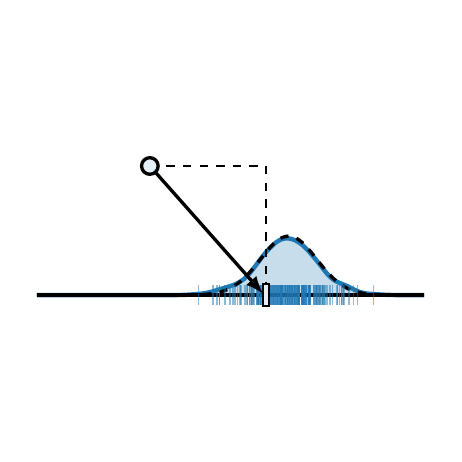
\begin{tikzpicture}
\begin{axis}[axis lines={none}, height={6.5cm}, width={6.5cm}, xmin={-3}, xmax={3}, ymin={-3}, ymax={3}, clip mode={individual}]
    \node at (-3,-3) {};
    \node at (-3,3) {};
    \node at (3,3) {};
    \node at (3,-3) {};
    \addplot[no markers, smooth, ultra thick, color={rgb,1:red,0.1216;green,0.4667;blue,0.7059}, fill={rgb,1:red,0.1216;green,0.4667;blue,0.7059}, fill opacity={0.25}]
        coordinates {
            (-3.0,-0.9999996652020177)
            (-2.9,-1.0)
            (-2.8,-0.9999997473907613)
            (-2.7,-1.0)
            (-2.6,-0.9999998060302603)
            (-2.5,-1.0)
            (-2.4,-0.9999998489954379)
            (-2.3,-1.0)
            (-2.2,-0.9999998807819237)
            (-2.1,-1.0)
            (-2.0,-0.9999999036470928)
            (-1.9,-1.0)
            (-1.8,-0.9999999180628167)
            (-1.7,-1.0)
            (-1.6,-0.9999999225693723)
            (-1.5,-1.0)
            (-1.4,-0.9999999130507876)
            (-1.3,-1.0)
            (-1.2,-0.9999998785779327)
            (-1.1,-0.9999999618301265)
            (-1.0,-0.9999944363879862)
            (-0.9,-0.9999142474709689)
            (-0.8,-0.9992536493389257)
            (-0.7,-0.9964406151579576)
            (-0.6,-0.9902743273667755)
            (-0.5,-0.9824809116853117)
            (-0.4,-0.9714896880297803)
            (-0.3,-0.9500858698006442)
            (-0.2,-0.920171598748008)
            (-0.1,-0.8903080030605133)
            (0.0,-0.8596961735320843)
            (0.1,-0.8199558592828701)
            (0.2,-0.7571852737708227)
            (0.3,-0.657805397218492)
            (0.4,-0.5287583937683515)
            (0.5,-0.3959436960884075)
            (0.6,-0.2797255759077598)
            (0.7,-0.1877676298750478)
            (0.8,-0.13140858131324085)
            (0.9,-0.12131699338214974)
            (1.0,-0.15060407874217652)
            (1.1,-0.21301846411873804)
            (1.2,-0.3088372996533647)
            (1.3,-0.42422623669650295)
            (1.4,-0.5481297047661384)
            (1.5,-0.6735010956245199)
            (1.6,-0.7669047145878339)
            (1.7,-0.8165942042654252)
            (1.8,-0.8577117016755756)
            (1.9,-0.9078233449822264)
            (2.0,-0.9509682221802819)
            (2.1,-0.9743203974646967)
            (2.2,-0.9833785516480927)
            (2.3,-0.9896665699440512)
            (2.4,-0.9956402920436492)
            (2.5,-0.9988841565223477)
            (2.6,-0.999830750301803)
            (2.7,-0.999983959600127)
            (2.8,-0.9999997103405273)
            (2.9,-0.9999995213621055)
            (3.0,-1.0)
        }
        ;
    \addplot[no markers, smooth, black, very thick, dashed]
        coordinates {
            (-3.0,-1.0)
            (-2.9,-1.0)
            (-2.8,-0.9999999999999998)
            (-2.7,-0.9999999999999986)
            (-2.6,-0.9999999999999909)
            (-2.5,-0.9999999999999438)
            (-2.4,-0.9999999999996723)
            (-2.3,-0.9999999999981868)
            (-2.2,-0.999999999990484)
            (-2.1,-0.9999999999526182)
            (-2.0,-0.9999999997761739)
            (-1.9,-0.9999999989968812)
            (-1.8,-0.9999999957348286)
            (-1.7,-0.99999998279467)
            (-1.6,-0.9999999341536179)
            (-1.5,-0.9999997609200129)
            (-1.4,-0.9999991764368138)
            (-1.3,-0.9999973085084408)
            (-1.2,-0.9999916549005841)
            (-1.1,-0.9999754522097821)
            (-1.0,-0.9999314928836516)
            (-0.9,-0.9998186150009755)
            (-0.8,-0.9995443730100476)
            (-0.7,-0.9989141748075886)
            (-0.6,-0.9975449927421185)
            (-0.5,-0.99473391284028)
            (-0.4,-0.9892831858053971)
            (-0.3,-0.9793087963610623)
            (-0.2,-0.9620992150531535)
            (-0.1,-0.9341352496846472)
            (0.0,-0.8914073851657249)
            (0.1,-0.8301404663464845)
            (0.2,-0.7479295366289559)
            (0.3,-0.6451078543883948)
            (0.4,-0.5259619407034923)
            (0.5,-0.3992795303462793)
            (0.6,-0.2777724583187935)
            (0.7,-0.17620707699520421)
            (0.8,-0.1085346586964997)
            (0.9,-0.08476363969709866)
            (1.0,-0.1085346586964997)
            (1.1,-0.17620707699520421)
            (1.2,-0.2777724583187935)
            (1.3,-0.3992795303462793)
            (1.4,-0.5259619407034923)
            (1.5,-0.6451078543883946)
            (1.6,-0.747929536628956)
            (1.7,-0.8301404663464844)
            (1.8,-0.8914073851657249)
            (1.9,-0.9341352496846472)
            (2.0,-0.9620992150531535)
            (2.1,-0.9793087963610624)
            (2.2,-0.9892831858053971)
            (2.3,-0.99473391284028)
            (2.4,-0.9975449927421185)
            (2.5,-0.9989141748075886)
            (2.6,-0.9995443730100476)
            (2.7,-0.9998186150009755)
            (2.8,-0.9999314928836516)
            (2.9,-0.9999754522097821)
            (3.0,-0.9999916549005841)
        }
        ;
    \draw[black, ultra thick] ({rel axis cs:1,0}|-{axis cs:0,-1}) -- ({rel axis cs:0,0}|-{axis cs:0,-1});
    \addplot[only marks, mark={|}, mark size={3.5pt}, color={rgb,1:red,0.1216;green,0.4667;blue,0.7059}, opacity={0.5}]
        coordinates {
            (1.10649900126324,-1)
            (0.782351770498297,-1)
            (0.8626341572894871,-1)
            (0.44668666036589877,-1)
            (1.16994051468878,-1)
            (1.3887968969770008,-1)
            (0.7822570988514695,-1)
            (0.9578031461244666,-1)
            (0.07232941719046981,-1)
            (0.6257254070440768,-1)
            (0.8835976902169411,-1)
            (1.2434116626087959,-1)
            (1.4124426907398924,-1)
            (0.5936554336630903,-1)
            (0.6473280079451371,-1)
            (0.03876242932141563,-1)
            (1.3668869719463073,-1)
            (1.3073834578359966,-1)
            (0.7186654776407757,-1)
            (0.06638835498560403,-1)
            (0.5235541996814397,-1)
            (1.047474848497283,-1)
            (1.739639685667434,-1)
            (0.5434325019728957,-1)
            (1.1815577663611696,-1)
            (1.1303458858672533,-1)
            (1.1873365204077877,-1)
            (0.7525962342259555,-1)
            (0.29544844108948753,-1)
            (1.4193405512824837,-1)
            (0.4106175892179871,-1)
            (0.17354749927375646,-1)
            (0.6838139195259134,-1)
            (0.6990401011084175,-1)
            (0.4318807168574377,-1)
            (1.2145708591434732,-1)
            (0.6026177847672027,-1)
            (0.4251828545846079,-1)
            (1.7170729882118845,-1)
            (0.9535028637685146,-1)
            (0.9199455773713928,-1)
            (1.4373486429952123,-1)
            (0.9841530892033101,-1)
            (0.8962489745654533,-1)
            (1.0937838030130547,-1)
            (1.129590253249886,-1)
            (1.5374404927166827,-1)
            (1.0745202645514302,-1)
            (0.6102203271555665,-1)
            (1.1635520269804367,-1)
            (0.6988984492564939,-1)
            (-0.16543521170746023,-1)
            (1.0143872126234956,-1)
            (0.46620373678409455,-1)
            (0.6494243874605584,-1)
            (0.83991081965393,-1)
            (1.430057579228599,-1)
            (0.5359534566361374,-1)
            (0.8381869605428306,-1)
            (0.8224901076605526,-1)
            (0.14086999250865828,-1)
            (0.8544502113341323,-1)
            (0.4583476663374988,-1)
            (-0.49344593164802375,-1)
            (0.2590568528851439,-1)
            (0.9287980906992506,-1)
            (1.3439361088963335,-1)
            (0.22032088510247916,-1)
            (0.8489573320256686,-1)
            (1.8986407899419127,-1)
            (0.8066435508519946,-1)
            (1.3280784313702612,-1)
            (0.3471492171087478,-1)
            (0.5985549934964669,-1)
            (1.240820741840948,-1)
            (0.7927178655205441,-1)
            (0.813838390923781,-1)
            (0.7980835863628928,-1)
            (0.7004207642646387,-1)
            (1.5428858504251326,-1)
            (0.6653722686099285,-1)
            (0.8052782022620668,-1)
            (1.1732674731266424,-1)
            (0.7263091205506955,-1)
            (1.3768143371812787,-1)
            (1.0680573893861447,-1)
            (0.6327380890343982,-1)
            (1.445365478503668,-1)
            (1.2283549271736443,-1)
            (0.5948945634614252,-1)
            (1.1680978790883643,-1)
            (1.3464503104726266,-1)
            (1.3382696597640003,-1)
            (1.8213068134659185,-1)
            (0.6199181064043969,-1)
            (0.895406659363791,-1)
            (1.234067571666356,-1)
            (0.42487944935460326,-1)
            (0.32835292008942507,-1)
            (1.770250238425151,-1)
            (0.7149195231822254,-1)
            (0.9176235492917826,-1)
            (1.0247413793113238,-1)
            (0.23119488223861673,-1)
            (0.002230860055336681,-1)
            (0.40640429972258507,-1)
            (0.36951442442088567,-1)
            (0.9666767631510775,-1)
            (1.2175826070756388,-1)
            (1.0677889612811406,-1)
            (0.47184016641115706,-1)
            (1.22360018260661,-1)
            (0.94715067849977,-1)
            (0.5427790343788725,-1)
            (1.052292761079582,-1)
            (0.5382461869287831,-1)
            (0.7306818279058735,-1)
            (0.7125162355142908,-1)
            (0.5984942514189695,-1)
            (0.35378953701573024,-1)
            (1.2046554757547026,-1)
            (0.7381920997633855,-1)
            (0.6806592945082277,-1)
            (1.1391206284467288,-1)
            (-0.07852444353044374,-1)
            (0.6638741944660793,-1)
            (0.9270645248551528,-1)
            (0.148711493517562,-1)
            (0.4315738287280916,-1)
            (0.5023671092310313,-1)
            (0.8554266789920011,-1)
            (0.8471007071808673,-1)
            (0.628410854938489,-1)
            (0.4950668112375148,-1)
            (0.7943243801784377,-1)
            (0.8906263159048224,-1)
            (1.6951058303307014,-1)
            (1.125294443130591,-1)
            (0.8627379694697044,-1)
            (1.5788245390357327,-1)
            (0.9914414874821137,-1)
            (1.1234312275857568,-1)
            (0.9711873878351254,-1)
            (0.970967307218993,-1)
            (0.9131699230430714,-1)
            (1.0447147430109653,-1)
            (1.2067501860477077,-1)
            (0.6237639971461315,-1)
            (2.211282946382047,-1)
            (1.1526190640362497,-1)
            (0.9368187650949755,-1)
            (1.4504733283994569,-1)
            (0.6578196340350382,-1)
            (0.846816219453828,-1)
            (1.420179041957926,-1)
            (0.8867581786153556,-1)
            (-0.21021994521429876,-1)
            (1.034208627016814,-1)
            (1.1142868521192575,-1)
            (0.5542062611444858,-1)
            (-0.16834648555725096,-1)
            (0.5145127916937213,-1)
            (1.653757645380104,-1)
            (0.9519904316347454,-1)
            (1.0606737583906536,-1)
            (1.0577129347167131,-1)
            (1.0300384967544614,-1)
            (0.47978723127853584,-1)
            (1.2818925180843275,-1)
            (0.6401438488522613,-1)
            (0.7715345528667648,-1)
            (0.3181240235017958,-1)
            (0.30130319306944275,-1)
            (1.3306779469887675,-1)
            (0.6042167171,-1)
            (1.2932517356875355,-1)
            (0.9200558191746607,-1)
            (1.1035921463998712,-1)
            (0.5585077219139595,-1)
            (1.3124089187822345,-1)
            (1.0517523989843283,-1)
            (0.7485774146647983,-1)
            (1.122080147034778,-1)
            (0.4975435850737181,-1)
            (1.3761127200888044,-1)
            (0.7591253638419013,-1)
            (1.3334973749347978,-1)
            (0.4505860074298901,-1)
            (-0.2713259351575785,-1)
            (0.10946535583086447,-1)
            (1.449352626234708,-1)
            (-0.015501831372745078,-1)
            (0.9856738615619905,-1)
            (1.0387359812313823,-1)
            (1.5066110086612805,-1)
            (0.8515986544109105,-1)
            (1.3222767616396995,-1)
            (0.8877217372769763,-1)
            (1.4849146582385313,-1)
            (0.3252290025253378,-1)
            (0.16050925922290563,-1)
            (1.1389851864723566,-1)
            (0.7783676974978395,-1)
            (1.224476904658536,-1)
            (0.9482109248432815,-1)
            (1.0029857720627187,-1)
            (1.1442067414649462,-1)
            (0.8769828433187945,-1)
            (1.7555734456991416,-1)
            (0.8813688539947307,-1)
            (1.2212452871206043,-1)
            (1.0968646038049954,-1)
            (1.8375612323443482,-1)
            (1.6619002709835073,-1)
            (1.065151009331161,-1)
            (0.9910858556943106,-1)
            (0.7833204549059523,-1)
            (0.42478451308660453,-1)
            (-0.09847453783128923,-1)
            (0.8075246331027393,-1)
            (0.5469235336489037,-1)
            (1.4721603408299622,-1)
            (1.0025827907282627,-1)
            (1.38448771629009,-1)
            (0.4162225162508598,-1)
            (0.34864029887260184,-1)
            (0.7261510171802315,-1)
            (0.5412786425671469,-1)
            (0.7890321129654516,-1)
            (1.3949589622143055,-1)
            (0.7508916181905574,-1)
            (1.360686236473896,-1)
            (1.6359858946869092,-1)
            (0.9901654178286925,-1)
            (0.7242832544491378,-1)
            (0.6866471952024515,-1)
            (1.1250272993148678,-1)
            (0.5426223863652896,-1)
            (1.0496906328395834,-1)
            (0.7900036102756859,-1)
            (1.7562033368554246,-1)
            (0.9622653592493076,-1)
            (0.254606362814324,-1)
            (1.7199286336677677,-1)
            (0.7806196964079746,-1)
            (1.214400253185725,-1)
            (1.9716178578506423,-1)
            (0.46747143513807854,-1)
            (1.216724926711625,-1)
            (0.6605188335458677,-1)
        }
        ;
    \addplot[no markers, dashed, black, thick]
        coordinates {
            (-1.25,1.0)
            (0.55,1.0)
            (0.55,-1)
        }
        ;
    \addplot[quiver={u={\thisrow{u}}, v={\thisrow{v}}}, very thick, -latex]
        table[row sep={\\}]
        {
            x  y  u  v  \\
            -1.25  1.0  1.755  -1.98  \\
        }
        ;
    \draw
    [thick, fill={rgb,1:red,0.8902;green,0.9333;blue,0.9647}] ({axis cs:0.505,-1.17}) rectangle ({axis cs:0.5950000000000001,-0.83});
    \addplot[only marks, very thick, mark size={3pt}, fill={rgb,1:red,0.8902;green,0.9333;blue,0.9647}]
        coordinates {
            (-1.25,1.0)
        }
        ;
\end{axis}
\end{tikzpicture}
\end{document}

\caption{Transform into conditional distribution.}
\end{subfigure}
\caption{Illustration of pathwise conditioning of a bivariate Gaussian. Here, we first sample a random vector from the joint distribution, then transform it into a sample from the conditional distribution.
These steps are called \emph{pathwise} because they are defined directly using random variables, rather than indirectly through probability distributions.}
\label{fig:pw-cond-mvn}
\end{figure*}

From \Cref{thm:mvn-pw}, we obtain a second way of representing multivariate Gaussian conditionals.
This entails two steps: (i) sample $\v\theta,\v{y}$ jointly, and (ii) transform $\v\theta,\v{y}$ into $\v\theta\given\v{y}=\v\gamma$ by employing the given expression.
This procedure is illustrated in \Cref{fig:pw-cond-mvn}.

Remarkably, this result is missing from every machine learning textbook on Gaussian processes that I am aware of, and appears almost entirely unknown within the field.
It's possible this is because the expression's computational costs are cubic in the combined dimension, which is more expensive than the previous costs.
While this holds for general Gaussians, we will show it can be avoided for many cases of practical interest in the sequel.

On the other hand, \Cref{thm:mvn-pw} is certainly known in other communities.
In a tribute to Georges Matheron, who pioneered the expression's use in geostatistics, \textcite{chiles05} say that:

\begin{quotation}
[Matheron's update rule] is nowhere to be found in Matheron's entire published works, as he merely regarded it as an immediate consequence of the orthogonality of the [conditional expectation] and the [residual process].
\end{quotation}

More recently, \textcite{doucet10} describes the algorithm in a technical report which begins with the remark: 

\begin{quotation}
This note contains no original material and will never be submitted anywhere for publication. However, it might be of interest to people working with [Gaussian processes] so I am making it publicly available.
\end{quotation}

The present state of affairs therefore seems to be that a small set of technical experts are aware of \Cref{thm:mvn-pw} but believe it to be too trivial to write about, while practitioners working in areas such as Bayesian optimization do not know that it exists.
While for multivariate Gaussians the result certainly is trivial, we will subsequently show that using it in the right manner yields significant progress towards resolving certain long-standing issues in decision-making settings.
To do so, we now consider Gaussian processes.

\section{Conditioning Gaussian processes}

We now study conditioning in Gaussian processes.
Specifically, we will develop and showcase the two points of view introduced above---distributional and pathwise---in the Gaussian process setting.
We begin with the former.

\subsection{Distributional conditioning}

The standard way of representing Gaussian process conditionals is to use the finiteness of the data to pick a sufficiently large grid of points, and work with finite-dimensional marginals.
Conditioning the Gaussian process then reduces to conditioning multivariate Gaussians.
We now describe this, setting the prior mean to zero to ease notation.

\begin{proposition}[Posterior Gaussian process~(finite-dimen\-sional~marginals)]
\label{prop:gp-cond}
The Bayesian model
\[
\v{y} \given f &\~[N](\v{f}, \m\Sigma)
&
f &\~[GP](0,k)
\]
where $\v{f} = (f(x_1),..,f(x_n))$ admits a Gaussian process as its posterior. 
Denoting $f\given y_1 = \gamma_1,..,y_n = \gamma_n$ by $f\given \v{y}$ for brevity, this process satisfies
\[
f\given\v{y}\~[N](\m{K}_{(\.)x} \m{K}_{xx}^{-1}\v\gamma, \m{K}_{(\.,\.)} - \m{K}_{(\.)x} (\m{K}_{xx} + \m\Sigma)^{-1} \m{K}_{x(\.)})
.
\]
\end{proposition}

\begin{proof}
Apply \Cref{prop:mvn-cond} to a set of finite-dimensional marginals.
\end{proof}

\begin{figure*}[t]
\vspace*{10ex}
[GP Distributional Conditioning Plot]
\vspace*{10ex}
\caption{TODO.}
\label{fig:dist-cond-gp}
\end{figure*}

This result gives us a way of carrying out Bayesian learning using Gaussian processes, given a finite set of data.
Note the \emph{bottom-up} nature of this perspective: we describe the posterior Gaussian process---which is an actual \emph{process} defined everywhere---using its posterior finite-dimensional marginals.

We now consider computational costs of the above formula.
Calculating posterior moments clearly entails cubic costs with respect to the data size $n$, owing the need to invert $n\x n$ matrices.
Now, suppose we are are interested in computing quantities involving the posterior distribution.
Consider for instance computing the Thompson sampling acquisition function considered in \Cref{sec:bayesian-optimization}, which we recall is 
\[
x_{t+1}(\omega) &= \argmax_{x\in X} \phi_t(\omega,x)
&
\phi_t&\~ f \given \v{y}
.
\]
Given the minimization involved in this objective, there is no chance in finding an analytic expression for $x_{t+1}$, and we must resort to numerical methods.
Just about any numerical procedure one can imagine---for instance, gradient descent---will involve drawing random samples from $f\given\v{y}$ at different locations, and performing the necessary algorithmic operations on them.
Summarizing, the computational costs of this expression are as follows.

\1 Data: $\c{O}(n^3)$ where $n$ is the size of the training set.
\2 Predictions: $\c{O}(n_*^3)$ where $n_*$ is the number of locations the posterior needs to be jointly evaluated at.
\0

This becomes more difficult if one considers that the evaluation locations may not be known in advance, and might be determined using previous points.
Due to the need to factorize matrices at every intermediate computation step, roundoff errors will accumulate as computations proceed.
Thus, even if we are willing to pay cubic costs, we must then face the secondary issue of numerical instability.
The situation if one needs to differentiate through objectives such as $\phi_t$ is even worse.

Without additional considerations, these costs are disastrous, and illustrate the difficulties in making methods such as Bayesian optimization perform effectively in practice.
Fortunately, a wide variety of techniques to deal with them are available: in particular, \emph{inducing point} methods provide a broad set of approximations for reducing the $\c{O}(n^3)$ costs.
We will complement these ideas by introducing techniques to tackle the $\c{O}(n_*^3)$ costs in the sequel.
For this, we proceed to develop a pathwise view of conditioning.

\subsection{Pathwise conditioning}

Given the pathwise view of conditioning multivariate Gaussians given by Matheron's Update Rule, one can ask: is there an analogous statement for Gaussian processes?
Does the purely notion of a Gaussian conditional distribution have an analogous description in terms of random functions?
We answer this affirmatively below.

\begin{corollary}[Posterior Gaussian process (pathwise)]
\label{cor:gp-pw}
For $\v{y}\given f$, $f$, and $\v{f}$ defined in \Cref{prop:gp-cond}, we have
\[
(f \given\v{y})(\omega,\v\gamma) \overset{\d}{=} f(\omega,\.) + \m{K}_{(\.)\v{x}} (\m{K}_{\v{x}\v{x}} + \m\Sigma)^{-1}(\v\gamma - \v{f}(\omega) - \v\eps(\omega))
\]
where $\v\eps \~[N](\v{0},\m\Sigma)$.
\end{corollary}

\begin{proof}
Apply \Cref{thm:mvn-pw} to a set of finite-dimensional marginals.
\end{proof}

\begin{figure*}[t]
\vspace*{10ex}
[GP Pathwise Conditioning Plot]
\vspace*{10ex}
\caption{TODO.}
\label{fig:pw-cond-gp}
\end{figure*}

Note that in this expression, the prior is evaluated jointly at all locations---the random variables $f(\omega,\.)$ and $\v{f}(\omega)$ are \emph{dependent}.
Similarly, equality can clearly only hold in distribution because the random variable $(f\given\v{y})(\.,\v\gamma)$ is only defined in distribution to begin with.

\Cref{cor:gp-pw} gives an alternative way of representing posterior Gaussian processes: (i) sample the prior and all auxillary random variables, and (ii) transform the sampled function to form the posterior as a random function.
This is illustrated in Figure \ref{fig:pw-cond-gp}.

This strategy can be carried out if we know the locations we wish to evaluate the posterior at.
In this case, we sample the prior at the data and evaluation locations jointly, and transform the resulting samples into posterior samples.
Examining the computational costs, we see these are $\c{O}(n^3)$ with respect to data size, and $\c{O}(n_*^3)$ with respect to the number of evaluation locations.
At this stage, then, we have seemingly only gained numerical stability.

\Cref{cor:gp-pw}, however, is not merely a computational result: it gives us a \emph{different way of thinking} about posterior Gaussian processes. 
In particular, we can use the point of view it offers to construct posterior approximations.
Observe that the cubic costs $\c{O}(n_*^3)$ occur entirely due to the need to jointly sample the prior at all evaluation locations.
Suppose, then, that we can approximately express the prior as 
\[
f(\omega,\.) &\approx \tilde{f}(\omega,\.) = \sum_{i=1}^\ell w_i(\omega)\phi_i(\.)
&
w_j &\~[N](0,1)
.
\]
We can substitute this approximation into \Cref{cor:gp-pw} to obtain
\[
(f \given\v{y})(\omega,\v\gamma) \overset{\d}{\approx} \tilde{f}(\omega,\.) + \m{K}_{(\.)\v{x}} (\m{K}_{\v{x}\v{x}} + \m\Sigma)^{-1}(\v\gamma - \v{\tilde{f}}(\omega) - \v\eps(\omega))
\]
where $\tilde{f}_n = \tilde{f}(\.,x_n)$.
We illustrate this idea in Figure \ref{fig:pw-cond-gp-rff}.
Once the random weights $\v{w}$ are sampled, the posterior becomes a deterministic function, which can be evaluated at $\c{O}(n_*)$ costs.
Thus, under this approximations, our cubic costs with respect to the number of evaluation locations become \emph{linear}.
We show in the sequel that for appropriate choices of $\tilde{f}$, such approximations can achieve excellent error control, ensuring they perform effectively in practice.

\begin{figure*}[t]
\vspace*{10ex}
[RFF GP Pathwise Conditioning Plot]
\vspace*{10ex}
\caption{TODO.}
\label{fig:pw-cond-gp-rff}
\end{figure*}

We now examine a different aspect of the pathwise representation of posterior Gaussian processes: the role of the data.
By re-expressing the matrix-vector product of the kernel matrix term $\m{K}_{(\.)\v{x}}$ as a sum, we obtain
\[
(f \given\v{y})(\omega,\v\gamma) \overset{\d}{=} f(\omega,\.) + \sum_{j=1}^n v_j(\omega) k(x_j,\.)
\]
where $\v{v} = (\m{K}_{\v{x}\v{x}} + \m\Sigma)^{-1}(\v\gamma - \v{\tilde{f}}(\omega) - \v\eps(\omega))$.
This \ref{cor:gp-pw} identifies the effect of the data in a posterior Gaussian process as the addition of \emph{canonical basis functions} $k(x_i,\.)$ to the prior.
We explore this interpretation further in the sequel.
From this viewpoint, our approximate posterior is
\[
(f \given\v{y})(\omega,\v\gamma) \overset{\d}{\approx} \sum_{i=1}^\ell w_i(\omega)\phi_i(\.) + \sum_{j=1}^n v_j(\omega) k(x_j,\.)
\]
which shows that our proposed approximation involves writing the posterior Gaussian process of interest as a sum of \emph{two} finite sets of basis functions---one for the prior, another for the data.
The basis coefficients $w_i$ and $v_j$ here are dependent random variables.
Summarizing, pathwise representations of posterior Gaussian processes provide a useful framework for constructing posterior approximations.

In Bayesian optimization, the preceding techniques offer a promising avenue to avoid the computational difficulties described previously.
If we again consider Thompson sampling, computing quantities such as
\[
x_{t+1}(\omega) &= \argmax_{x\in X} \phi_t(\omega,x)
&
\phi_t&\~ f \given \v{y}
\]
can be done using a simple Monte Carlo approach as follows.

\1 Sample the random weights $(\v{w}, \v{v})$ to form the approximate posterior.
\2 Maximize the approximate posterior using any numerical procedure.
\0

The key advantage of this approach is that once the random weights are sampled, the posterior---a random function---effectively becomes deterministic.
This allows us to not only evaluate it in linear time, but also to differentiate through posterior samples using automatic differentiation---here, enabling us to maximize them using gradient descent without computing gradient processes or employing special considerations of any kind.

In total, we obtain a substantially more accurate and efficient way to compute acquisition functions such as Thompson sampling.
To obtain a complete algorithm, all that remains is to find finite basis approximations to Gaussian process priors: this will require additional structure present in specific classes of kernels.
We proceed to explore a number of techniques for doing so.

\section{Sampling from prior Gaussian processes}

In the preceding section, we explored a class of approximate posterior Gaussian processes constructed by plugging a finite-basis-function-based approximate prior into the pathwise update.
Such approximate priors can be constructed in many ways, including by expressing the true prior within a basis of an appropriate space of functions, and truncating the resulting infinite sum.
Within this class, different bases will have different properties.
This will affect applicability, ease of use, and approximation error.
We now explore a number of possible choices.


\subsection{Random feature methods}

For stationary kernels on Euclidean spaces, random feature methods can be used to construct approximate priors whose properties make them one of the most attractive choices possible.
We examine these now.

To construct a basis function expansion, our strategy will be to find a \emph{feature map} $\varphi : \c{X} \-> \c{H}_k$ that maps states into vectors in the \emph{reproducing kernel Hilbert space} induced by $k$.
This is defined as follows.

\begin{definition}[Reproducing kernel Hilbert space]
Let $X$ be a set, and let $\c{H} \subseteq \R^X$ be a Hilbert space of functions. 
We say that $\c{H}$ is a \emph{reproducing kernel Hilbert space} if, for any $x\in X$, we have $\f{ev}_x \in \c{H}^*$ where $\f{ev}_x : \c{H} \-> \R$ is called the \emph{evaluation map} and is defined by $\f{ev}_x f = f(x)$.
\end{definition}

Ostensibly, this definition has nothing to do with kernels, and it is unclear what a reproducing kernel Hilbert space \emph{induced by} $k$ actually means.
A consequence of the above definition is that given a reproducing kernel Hilbert space $\c{H}$, we can define the function $k_{\c{H}}(x,x') = \innerprod[1]{\Psi_{\c{H}}^{-1}\f{ev}_x}{\Psi^{-1}_{\c{H}}\f{ev}_{x'}}$, called the \emphmarginnote{reproducing kernel}, where $\Psi_{\c{H}} : \c{H} \-> \c{H}^*$ is the bijective linear isometry given by the Riesz Representation Theorem.
It is easy to see that $k_{\c{H}}$ is positive semi-definite.\footnote{TODO: check if it's PD or PSD.}
It turns out a converse statement also holds.

\begin{result}[Moore-Aronszajn Theorem]
Let $k : X \x X \-> \R$ be a symmetric positive semi-definite kernel.
Then there is a unique Hilbert space $\c{H}_k \subseteq \R^X$ for which $k$ is the reproducing kernel.
\end{result}

\begin{proof}
TODO: cite.
\end{proof}

This gives another point of view from which one can study and understand kernels.
We will need one final notion.
We say that a function $\varphi : X \-> \c{H}_k$ is a \emphmarginnote{feature map} if $k(x,x') = \innerprod{\phi(x)}{\phi(x')}$.
Now, we introduce the key idea for constructing our approximate Gaussian prior: suppose we have a \emph{finite-dimensional} approximation for such a feature map, namely a vector-valued function $\v\phi : X \-> \R^\ell$ such that $\v\phi(x)^T \v\phi(x') = \innerprod{\phi(x)}{\phi(x')}$.
Then
\[
\tilde{f}(\.) &= \sum_{i=1}^\ell w_i(\omega) \phi_i(\.)
&
w_i &\~[N](0,1)
\]
by direct calculation has covariance approximately equal to that of $f$.
Therefore, to construct an approximate prior, it suffices to find a finite-dimensional approximate feature map.

For stationary kernels, techniques for constructing approximate feature maps are well-studied, originally motivated by questions arising in kernel support vector machines.
We now introduce the \emph{random Fourier feature} method for constructing such maps, beginning with a description of the stationary setting.

\parmarginnote{Stationary kernel}
Let $X = \R^d$.
We say that a kernel $k(\v{x},\v{x}')$ is called \emph{stationary} if $k(\v{x},\v{x}') = k(\v{x} - \v{x})$ for a function $k : \R^d \-> \R$.
A stationary kernel, then, is a two-argument positive definite function which factorizes through a one-argument function depending only on the difference between two points.
Note that such a kernel is invariant under translation and can be characterized as such.
We will need a result known as \emph{Bochner's Theorem}.

\begin{result}[Bochner's Theorem]
For every stationary continuous positive definite kernel with $k(\v{x},\v{x}) = 1$ there is a symmetric probability measure $\rho$ on $\R^d$ which we call the \emph{spectral measure} of $k$.
Moreover, $k$ admits the representation
\[
k(\v{x} - \v{x}') = \int_{\R^d} e^{2\pi i \v\varpi^T (\v{x} - \v{x}')} \d\rho(\v\varpi)
.
\]
Conversely, every probability measure on $\R^d$ gives rise to such a kernel via its inverse Fourier transform.
\end{result}

\begin{proof}
TODO: cite.
\end{proof}

Here, \emph{symmetry} of $\rho$ refers to invariance under reflection about the origin.
This result is true more generally if $X$ is replaced by a locally compact Abelian group, for which the corresponding spectral measure will be supported on the Pontryagin dual group---we omit this level of generality because we will not need it.
We do briefly note, however, that this means that spectral measures of kernels on compact spaces are \emph{discrete}---this behavior will reappear under a different guise in \Cref{ch:noneuclidean}.

\begin{figure*}[t]
\vspace*{10ex}
[RFF Prior Sampling Plot]
\vspace*{10ex}
\caption{TODO.}
\end{figure*}

From here, it is clear that the feature map we seek can be constructed by Monte Carlo sampling the integral representation given by Bochner's Theorem.
To maintain order, we introduce a \emph{second} probability space $(\Xi,\c{G},\bb{Q})$ to distinguish the stochasticity associated with the random feature expansion from stochasticity associated with the Gaussian process.
Letting $\Re$ denote the real part of a complex number, our approximate prior is\footnote{TODO: check if this is really the one we want.}
\[
\tilde{f}(\.) &= \frac{1}{\sqrt{\ell}} \Re \del{\sum_{i=1}^\ell w_i(\omega) e^{2\pi i \v\varpi(\xi)^T(\.)}}
&
w_i &\~[N](0,1)
&
\v\varpi &\~ \rho
\]

What is remarkable about random feature methods is that, owing to the Monte Carlo nature of the approximation, the decay rate of appropriately defined approximation error is \emph{dimension-free}.
This limits the effect of the curse of dimensionality to constant factors.
Better yet, random feature methods are well-understood owing to their widespread use in other areas, and error bounds are available.
For this reason, they are often the technique of choice for stationary Euclidean kernels.
We now consider other cases.

\subsection{Karhunen--Loève expansions}

Among all techniques for constructing approximate priors, different techniques will generally yield different amounts of error for the same number of basis functions.
One can then ask: is there an optimal choice?
Of course, the answer to this question will depend on what one actually means by the word \emph{optimal}.

If we take $X \subset \R^d$ to be closed and compact, and we use expected mean squared error---which we recall is equivalent to the $L^1(\Omega;L^2(X;\R))$ norm---as our notion of optimality, one can affirmatively answer the above question.
Recall that a continuous kernel $k : X \x X \-> \R$ induces a covariance operator
\[
\c{K} : L^2(X;\R) &\-> L^2(X;\R)
&
\c{K} : \phi &\|> \int_X \phi(x) k(x,\.) \d x
\]
where by writing $\norm{\c{K} \phi}_{L^1(X;\R)} \leq \vol(X) \norm{k}_{C^0(X\x X;\R)} \norm{\phi}_{L^2(X;\R)}$ using compactness and boundedness of $k$ we affirm correctness of the operator's domain and range.
By compactness, $\c{K}$ will admit a countable set of eigenvalues and eigenfunctions.
It turns out, that, by the Karhunen--Loève Theorem, the Gaussian process itself can be written in terms of the same eigenvalues and eigenfunctions as well.

\begin{result}[Karhunen--Loève Theorem]
Let $X \subseteq \R^d$ be closed and compact, and let $f$ be a Gaussian process with continuous covariance function.
Then we have
\[
f(\omega,\.) &= \sum_{i=1}^\infty w_i(\omega) \phi_i(\.)
&
w_i &\~[N](0,1)
\]
where convergence holds almost surely, and $\phi_i$ are an orthogonal basis on $L^2(X;\R)$ given by the eigenfunctions of the covariance operator.
Moreover, for every $\ell\in \N$, truncating this series yields an $L^1(\Omega;L^2(X;\R))$-optimal approximation among all $\ell$-term sums of $L^2(X;\R)$-orthogonal functions.
\end{result}

\begin{proof}
TODO: cite.
\end{proof}

More generally, an analogous result, albeit with a weaker form of convergence, also holds for general \emph{square-integrable} stochastic processes which may be non-Gaussian.
Since we will not consider such processes, we do not pursue this direction here.

\begin{figure*}[t]
\vspace*{10ex}
[KL Expansion Boundary Constrained Plot]
\vspace*{10ex}
\caption{TODO.}
\end{figure*}

For a general kernel, finding the eigenfunctions of the covariance operator may be difficult.
For certain classes of Gaussian processes constructed to satisfy appropriate boundary constraints, however, the eigenfunctions of the covariance operator will coincide with the eigenfunctions of a boundary-constrained Laplacian.
These can be obtained numerically, giving a suitable way for sampling from priors in the boundary-constrained setting.

Kernels induced by eigenvalues and eigenfunctions of appropriately-defined Laplace operators are also a common tool in non-Euclidean settings, and we will explore them further in \Cref{ch:noneuclidean}.
For the moment, however, we consider a third class of approximations.

\subsection{Finite element methods}

We now introduce the third class of approximations we will consider: those constructed via \emph{finite element approximations} of solutions of stochastic partial differential equations.
Many Gaussian process priors, including the widely-used Matérn class, can be expressed in such a manner.
Gaussian processes which satisfy stochastic partial differential equations are also of direct interest in non-Euclidean settings considered in \Cref{ch:noneuclidean}.

Let $X$ be a sufficiently well-behaved subset of a Euclidean space, or a Riemannian manifold.
Suppose our Gaussian process $f$, when reinterpreted as a generalized Gaussian field, satisfies the equation 
\[
\c{L}f = \c{W} 
\]
where $\c{L} : H \-> L^2(X)$ is a bounded linear operator acting on a reproducing kernel Hilbert space, and $\c{W}$ is a white noise process over $L^2(X)$.
More precisely, this equation is meant in the sense of an almost sure equality
\[
f(\omega,\c{L}^* h) = \c{W}(\omega, h)
\]
between generalized Gaussian fields---a formal treatment is given in \Cref{ch:noneuclidean}.
Assume that the generalized Gaussian field $f : \Omega \x H \-> \R$ can be written as the integral of a Gaussian process $f : \Omega \x X \-> \R$ as
\[
f(\omega, h) = \int_X f(\omega, x) h(x) \d x
\]
which holds provided that $f$ is measurable.
This, in turn, depends on regularity properties of the kernel, but will hold in essentially all practical cases of interest, and in particular on closed compact domains $X$ follows from sample-continuity.
If we define the bilinear form 
\[
a(\phi,\psi) = \int_X \phi(x) (\c{L}^*\psi)(x) \d x    
\]
then our stochastic partial differential equation becomes
\[
a(f(\omega,\.), h) = \c{W}(\omega, h)
\]
which is an equation between a Gaussian process, bilinear form, and random linear functional.
Now, we introduce approximations: suppose that $f(\omega,x) \approx \tilde{f}(\omega,x) = \sum_{i=1}^\ell w_i(\omega) \phi_i(x)$ and that $h(x) \approx \sum_{j=1}^\ell v_j \psi_j(x)$.
Plugging this in and differentiating to remove the coefficients $v_j$ yields 
\[
\sum_{i=1}^\ell w_i(\omega) a(\phi_i,\psi_j) = \c{W}(\omega, \psi_j)
\]
which by defining $A_{ij} = a(\phi_i,\psi_j)$ and $b_j(\omega) = \c{W}(\omega, \psi_j)$ can be recognized as a random linear system, more compactly written
\[
\m{A} \v{w} = \v{b}
.
\]
If we let $\m{M} = \Cov(\v{b})$ where $\Cov(b_i,b_j) = \innerprod{\psi_i}{\psi_j}$---where we note that since $\c{W}$ is a white noise process, the matrix $\m{M}$ coincides with the finite-element mass matrix---we obtain the distribution for the basis coefficients. 
Our approximate prior can therefore be written
\[
\tilde{f}(\omega,x) &= \sum_{i=1}^\ell w_i(\omega) \phi_i(x)
&
\v{w} &\~[N](\v{0},\m{A}^{-1}\m{M}\m{A}^{-T})\
.
\]
What is particularly powerful about this technique is that it gives us a significant degree of freedom for what kinds of finite sets of basis functions we can choose for $\phi$ and $\psi$.
A fruitful choice, provided the operator $\c{L}$ is a differential operator of sufficiently low order that this makes sense, is to take them to be compactly supported piecewise linear functions, since this will cause the matrices $\m{A}$ and $\m{M}$ to be sparse.
This can enable one to use a much larger set of basis functions compared to alternative methods.

\begin{figure*}[t]
\vspace*{10ex}
[Finite Element Plot]
\vspace*{10ex}
\caption{TODO.}
\end{figure*}

The main difficulty with finite element methods is that they typically demand more from practitioners compared to alternatives.
In particular, one usually needs to understand the stochastic partial differential equations governing the Gaussian process of interest with a reasonable degree of detail to know how to choose basis functions well.
Additionally, sparse linear algebra in a parallel environment with automatic differentiation can be cumbersome.

This concludes our presentation of techniques for constructing approximate priors.
In general, the best choice for a particular application will depend on the detailed requirements of the situation.
We now proceed to study other aspects of the pathwise viewpoint.

\section{Approximating pathwise data-dependent terms}

In the preceding section, we discussed techniques for approximating the prior using a finite set of basis functions with random coefficients.
Such approximations enabled us to construct approximate pathwise representations of posterior Gaussian processes with $\c{O}(n_*)$ computational complexity, where we recall again that $n_*$ is the number of points where we wish to evaluate the posterior at.
We now consider the other computational costs in the formula: $\c{O}(n^3)$, where $n$ is the size of the training data.
These arise because computing
\[
(f \given\v{y})(\omega,\v\gamma) \overset{\d}{=} f(\omega,\.) + \m{K}_{(\.)\v{x}} (\m{K}_{\v{x}\v{x}} + \m\Sigma)^{-1}(\v\gamma - \v{f}(\omega) - \v\eps(\omega))
\]
requires us to invert an $n\x n$ matrix.
We now ask: from a pathwise perspective, what techniques are available for reducing these costs?

\subsection{Inducing points}

Consider a simple approach to reducing the above cubic costs: instead of conditioning the Gaussian process on the full set of values $(x_1,y_1),..,(x_n,y_n)$, find a different data set $(z_1,\mu_1),..,(z_m,\mu_m)$, for which $m \ll  n$ and yet the posterior is approximately the same.
To ensure this approximation is expressive enough, we can either (i) make $\v\mu$ random with a learnable mean and covariance, or (ii) introduce a learned noise covariance $\m\Lambda$, rather than reusing the one from the original model.
The latter gives
\[
(f \given\v{u})(\omega,\v\mu) = f(\omega,\.) + \m{K}_{(\.)\v{z}} (\m{K}_{\v{z}\v{z}} + \m\Lambda)^{-1}(\v\mu - \v{f}(\omega) - \v\epsilon(\omega))
\]
where $f\given\v{u}$ is the posterior under the modified likelihood employing the noise covariance $\m\Lambda$.
This approximation has a particularly simple interpretation: we can re-write it as
\[
(f \given\v{u})(\omega,\v\mu) = f(\omega,\.) + \sum_{j=1}^m v_j(\omega) k(z_j,\.)
\]
where $\v{v}(\omega) = (\m{K}_{\v{z}\v{z}} + \m\Lambda)^{-1}(\v\mu - \v{f}(\omega) - \v\epsilon(\omega))$.
Thus, we see that all we have done is replaced a large sum of data-dependent functions $k(x_j,\.)$ with $j=1,..,n$ induced by the kernel with a much smaller sum involving a sparsified set of functions $k(z_j,\.)$ with $j=1,..,m$ and $m \ll n$.

Given such an approximate posterior, how should we select the introduced hyperparameters $\v{z},\v\mu,\m\Lambda$ to ensure quality?
At minimum, we should attempt to guarantee consistency of the approximation, in the sense that if $m = n$ then one can choose $\v{z} = \v{x}$, $\v\mu = \v\gamma$, and $\m\Lambda = \m\Sigma$ to recover the desired posterior.
We therefore seek to minimize some notion of \emph{distance} on the space of probability measures.

The most natural choice one can consider is arguably the one that emerged from the analysis of Bayes' Rule presented in \Cref{ch:intro}: namely, the \emph{Kullback--Leibler divergence}.
Minimizing this amounts to replacing the measure space in the variational formulation of Bayes' Rule of \Cref{prop:variational-bayes} with the parameterized subspace of measures induced by the set of approximate posteriors with different parameter values, which we the \emph{variational family}.
This yields the optimization problem 
\[
\argmin_{\bb{q}_f\in\bb{Q}} D_{\f{KL}}(\bb{q}_f \from \pi_f) + \frac{1}{2}\operatorname*{\E}_{f\~\bb{q}_f} (\v\gamma - f(\v{x}))^T \m\Sigma^{-1} (\v\gamma - f(\v{x}))
\]
where $\bb{Q}$ is the set of all measures equal to the distribution of $f\given\v{u}$ for some choice of variational parameter values $\v{z},\v\mu,\m\Lambda$, and $\bb{q}_f$ is the distribution of $f\given\v{u}$ for a specific set of such values.
Note that we have dropped constant terms from the likelihood density because they do not affect the optima.
Our \emph{variational approximation} is obtained by solving this optimization problem, which it turns out is necessarily well-posed.

\begin{proposition}[Variational objective for inducing point approximations]
For all $\v{x},\v{y},\m\Sigma$, and all $\v{z},\v\mu,\m\Lambda$, the Kullback--Leibler divergence $D_{\f{KL}}(\bb{q}_f \from \pi_{f \given\v{y}})$ is finite and equal to the above objective up to an additive constant.
Moreover, the prior Kullback--Leibler divergence $D_{\f{KL}}(\bb{q}_f \from \pi_f) = D_{\f{KL}}(\bb{q}_{f(\v{z})} \from \pi_{f(\v{z})})$ reduces to the Kullback--Leibler divergence between the respective finite-dimensional marginal distributions at the inducing locations $\v{z}$.
\end{proposition}

\begin{proof}
We consider the two terms in the objective and the additive constant.
\1 Finiteness of the first term, along with the second claim, follows by the chain rule for Kullback--Leibler divergences, since $\bb{q}_f$ is by construction a conditional distribution of a Gaussian process with the same covariance kernel as $k$.
\2 Finiteness of the second term follows immediately, because it is the expectation of a quadratic with respect to a multivariate Gaussian.
\3 Finiteness of the additive constant also follows, because it is by definition the log-density of a multivariate Gaussian.
\0 
The claim follows. 
\end{proof}

We have therefore proven that the \emph{inducing point} approximation of \textcite{opper09}, when re-interpreted using the variational inference framework of \textcite{titsias09}, coincides with the pathwise variational approximation constructed here.
The same is true for other classes of inducing points, including the family where $\v{u}$ is randomized, as originally proposed by \textcite{titsias09}.

\begin{figure*}[t]
\vspace*{10ex}
[Inducing Point Plot]
\vspace*{10ex}
\caption{TODO.}
\end{figure*}

Better yet, the constructions above are straightforward, principled, and mathematically sound.
In particular, we do not rely on heuristic arguments involving \emph{evidence lower bounds} which effectively require us to \emph{posit} that optimizing certain quantities will result in improved posterior approximation.
Instead, by virtue of the Kullback--Leibler divergence generating a Hausdorff topology on the space of probability measures, this is proven.

This concludes our study of inducing point methods from the pathwise perspective, which are identified with sparsified pathwise approximations where instead of a sum of $n$ kernel terms, we have a smaller sum of $m \ll n$ kernel terms.
We now consider another class of approximations that one can consider using in practice.

\subsection{Approximate priors}
In the preceding sections, we presented a number of posterior approximations which were built by approximating individual terms within the pathwise formalism.
We considered approximations where the prior term is replaced with a finite basis function approximation, and where the data term is replaced with a sparser analog.
An obvious question one can ask is, instead of approximating the prior term, why not just change the model by using a finite basis function prior to begin with?

The answer to this question is that the resulting model becomes fundamentally finite-dimensional, and loses expressive capacity, resulting in reduced performance.
This can be seen precisely by comparing its pathwise update 
\[
\tilde{f}(\omega,\.) + \ubr{\v\phi(\.)^T\v\phi(\v{x})}_{\t{replaces}\,\m{K}_{(\.)\v{x}}} (\ubr{\v\phi(\v{x})^T\v\phi(\v{x})}_{\t{replaces}\,\m{K}_{\v{x}\v{x}} } + \m\Sigma)^{-1}(\v\gamma - \v{\tilde{f}}(\omega) - \v\eps(\omega))
\]
to the pathwise update
\[
f(\omega,\.) + \m{K}_{(\.)\v{x}} (\m{K}_{\v{x}\v{x}} + \m\Sigma)^{-1}(\v\gamma - \v{\tilde{f}}(\omega) - \v\eps(\omega))
\]
under the original, infinite-dimensional prior.
Observe that all that has changed is that the kernel matrices $\m{K}_{(\.)\v{x}}$ and $\m{K}_{\v{x}\v{x}}$ have been replaced with the approximations $\v\phi(\.)^T\v\phi(\v{x})$ and $\v\phi(\v{x})^T\v\phi(\v{x})$.
Observe further that since $\tilde{f}(\omega,\.) = \v\phi(\.)^T\v{w}(\omega)$ where $w_i\~[N](0,1)$, we can write
\[
(f\given\v{y}) \approx \v\phi(\.)^T(\v{w}(\omega) + \v{\tilde{v}}(\omega))
\]
where $\v{\tilde{v}}(\omega) = \v{w}(\omega) + \v\phi(\v{x}) (\v\phi(\v{x})^T\v\phi(\v{x}) + \m\Sigma)^{-1}(\v\gamma - \v{\tilde{f}}(\omega) - \v\eps(\omega))$ are random weights.
Therefore, if change the model, then the posterior becomes a sum of the specified finite basis functions, irrespective of the data, and in particular does not grow as data size increases.

This therefore means its representational capacity---in the sense of the dimension of the vector space spanned by all basis functions used---also does not grow as data size increases.
This is to be contrasted with the approximate pathwise update, for which this dimensionality grows due to the presence of $n$ kernel functions $k(x_j,\.)$ in the sum.

\begin{figure*}[t]
\vspace*{10ex}
[Variance Starvation Plot]
\vspace*{10ex}
\caption{TODO.}
\label{fig:variance-starvation}
\end{figure*}

The result is that if the data size is large enough, performance degrades disastrously---this is seen in \Cref{fig:variance-starvation}
This phenomenon has been called \emph{variance starvation} in the literature, due to its ability to produce error bars that are too narrow as a result of lack of representational capacity---we note this name is misleading because it is also capable of producing error bars which are far too large.

By not approximating terms that do not need to be approximated, pathwise approximations avoid limiting representational capacity and thus retain performance.
Variance starvation has been a key performance issue in Bayesian optimization algorithms for some time---in our view, pathwise approximations of the kind described here largely resolve the issue.


\section{Error analysis}

Pathwise posterior approximations are, ultimately, approximations.
Therefore, a key question one can ask is: how accurate are they?
To quantify this, we need an appropriate notion of \emph{distance} to quantify how far away the two random variables of interest are.
This notion should possess a number of key properties.

\1  It should be \emph{distributional} in nature to reflect the fact that it is the information contained in the posterior that is of interest to us, rather than the precise way in which the random variables is generated.
\2 The distance between the true posterior and pathwise approximations should be finite, in order to facilitate meaningful comparisons.
\0 

The \emphmarginnote{Wasserstein distance} on the space of probability measures is defined as 
\[
W_{k,d}(\pi,\pi')^k = \inf_{\gamma\in\Gamma(\pi,\pi')} \int_{A\x A} d(a,a')^k \d\gamma(a,a')
\]
where $d$ is a metric on $A$, and $\Gamma(\pi,\pi')$ is this set of all \emph{couplings} of $\pi$ with $\pi'$, namely probability measured $\gamma$ supported on $A\x A$ whose marginals equal $\pi$ and $\pi'$.
We adopt this expression as our notion of distance.

The Wasserstein distance can be understood as the expected distance between two random variables $a$ and $a'$, with distributions $\pi$ and $\pi'$, where the random numbers used to generate $a$ and $a'$ are linked in order to make the expectation as small as possible.
The smallest possible expected distance is zero, which only occurs if the random variables can be made identical to one another---or, in other words, if their distributions coincide.

This definition satisfies both requirements. 
By virtue of varying random numbers---or, more precisely, optimizing over couplings---it compares distributions.
Moreover, unlike alternatives such as the Kullback--Leibler divergence or total variation distance, Wasserstein distances metrize the topology of weak convergence, do not impose restrictive absolute continuity requirements, and are finite in the cases of interest.

We will also analyze error in a second way: using the supremum norm between kernels.
Observe that pathwise approximations under mean-zero priors possess the exact same mean as the true posterior.
Therefore, when restricted to pathwise approximations under mean-zero priors, this notion lifts to a \emph{metric} rather than a pseudometric between probability distributions in the given class.
We now state our main result.

\begin{proposition}[Pathwise posterior Wasserstein error bound]
Assume $X \subseteq \R^d$ is compact and that $f \~[GP](\mu,k)$ is almost surely continuous.
Then we have 
\[
TODO
.
\]
\end{proposition}

\begin{proof}
TODO: clean up argument.
\end{proof}

\begin{proposition}[Pathwise posterior kernel error bound]
Assume $X \subseteq \R^d$ is compact and that $f \~[GP](\mu,k)$ is almost surely continuous.
Then we have 
\[
TODO
.
\]
\end{proposition}

\begin{proof}
TODO: clean up argument.
\end{proof}

The above arguments shows that, for a given dataset size, posterior approximation error is controlled by prior approximation error.
Thus, if we increase approximation accuracy in the prior, we are guaranteed to also increase approximation accuracy in the posterior, both in the limit and outside it..

The key idea in the above arguments was to analyze the pathwise approximation by applying standard function-analytic inequalities to the pathwise representation itself.
By varying the resulting norms, a wide set of similar inequalities follow: we make no attempt to optimize bounds, and instead focus on presenting the technique in the simplest manner.

\parmarginnote{Approximation error and asymptotic posterior contraction}
The bounds presented are not tight, particularly in large-data settings where the inverse matrix norm in the constant becomes large.
This may tempt one to conclude that approximation error will grow, but this is often false---instead, the bound becomes loose.
One way to see this is by considering posterior contraction: in large-data settings, the posterior will be concentrated, and since our approximations are exact with respect to the mean, there is little room left for error, in the absolute sense, to accumulate.

Different prior approximations possess different error behavior.
The random Fourier feature approach is particularly attractive because its Monte Carlo nature makes it decay at a dimension-free rate of $\sqrt{\ell}$---\textcite{sutherland15} provide bounds on this term.
Note also that the terms in our kernel bounds depend on the dimension only through the kernel matrix, which itself depends on the dimension of the data and not the ambient space.
In this sense, our bounds are very well-behaved with respect to dimension.

This concludes our theoretical presentation and analysis.
We now move to evaluating these ideas in practical settings, and discussing the broad picture painted by the ideas presented here and in the preceding sections.

\section{Bayesian optimization}

We now study empirically how pathwise approximations affect Bayesian optimization, using a simple experiment to showcase the key behavior.

TODO: new experiment

\section{Discussion}

Pathwise conditioning gives a powerful way to think about posterior Gaussian processes.
In the preceding sections, we used it to construct finite-dimensional approximations which yield actual random functions.
These functions are sums of finite basis functions and random coefficients---these coefficients can be sampled in advance, after which the functions can be evaluated at arbitrary points, as well as differentiated using standard techniques.

The resulting method is particularly useful in decision-making settings such as Bayesian optimization, where acquisition functions constructed from Gaussian process sample paths need to be optimized.
Using the presented technique, this can be done in linear time and without incurring large approximation error that degrades performance.
This is particularly useful in higher-dimensional settings.

The performance of pathwise approximate posterior Gaussian processes depends on the approximation accuracy of the prior term.
We presented a number of methods for doing so, each suited to their respective settings.
For stationary kernels, random Fourier feature methods are particularly attractive due to their good behavior with respect to dimension, but are by no means the only choice.
We hope these developments prompt further study of other possible choices.

TODO: talk about Bayesian optimization showcase






\chapter{Non-Euclidean Matérn Gaussian Processes}
\label{ch:noneuclidean}

\lettrine{A}{t present}, the most widely-used Gaussian process models employ stationary kernels defined on Euclidean spaces.
These kernels are attractive because they work effectively and it is generally easy to understand the kind of prior information they introduce into a problem.
This makes them a valuable tool for practitioners to use in the manner required for the task at hand.

Our goal throughout has been to expand the settings in which Gaussian process models and decision systems built atop them can be used.
We have so far focused on doing so by making existing models easier to work with, but now pursue a different approach: namely, we focus on expanding the scope of models one can consider to begin with.
We will again emphasize on constructiveness and making abstract ideas accessible to the practitioner.

We focus on the setting of Riemannian geometry, which describes a widely-occurring class of geometric shapes and spaces.
We thus study Gaussian processes whose domains are manifolds, rather than Euclidean spaces.
Working with manifolds often involves thinking carefully about discretization: we therefore also study purely discrete settings involving meshes and weighted undirected graphs, which are of inherent interest in their own right.

Our guiding theme will be: how can we make Gaussian processes on Riemannian manifolds be just as effective a model class as their Euclidean counterparts?
We now proceed to introduce, develop, and explore this topic.


\section{Riemannian Matérn Gaussian Processes}

We begin with a key question: how should one generalize the most widely-used class of Gaussian process models to the Riemannian manifold setting?
There are multiple potential definitions one can introduce, some of which will turn out to be much better-behaved mathematically than others.
In order to pursue these questions, we begin by introducing and reviewing the setting of differential geometry.

\subsection{Review of differential geometry}
We now briefly review the notions needed to define and understand manifolds.\footnote{The Russian word for \emph{manifold} is \emph{mnogoobrazie} (mnəg\rotatebox[origin=c]{180}{aa}br{\textquotesingle}az\textsuperscript{j}\textsc{i}jə). The word \emph{mnogo} means \emph{many}, and the word \emph{obraz} roughly means \emph{form}, \emph{view}, or \emph{image}. 
Thus, a \emph{manifold} is a \emph{space with many views into it}, which I find to be well-chosen and evocative.}
These are sets equipped with additional structure encoding their geometric shape.

A \emphmarginnote{topological space} is a set $X$ together with a \emph{topology}, which is a collection of subsets $\c{O}_X \subseteq 2^X$ called the \emph{open sets}---these include the empty set, the space itself, and are closed under pairwise intersections and arbitrary unions.
A given set generally admits many topologies.
Topological spaces admit notions of \emph{locality}, \emph{convergence}, \emph{continuity}, \emph{compactness}, \emph{denseness}, and many others.
The \emph{Hausdorff} property implies that limits are unique.

\parmarginnote{Topological manifold}
A paracompact Hausdorff topological space $(X,\c{O}_X)$ is called a $d$-dimensional \emph{topological manifold} if it is locally homeomorphic to $\R^d$ equipped with the standard topology.
For such a manifold, there is a set $\c{A}_X$ called the \emph{atlas} whose elements are the local homeomorphisms, called \emph{charts}.
An atlas is \emph{maximal} if it is the largest possible such set, in which case it is unique.

A \emphmarginnote{smooth differentiable manifold} is a triple  $(X,\c{O}_X,\c{A}_X)$ where $X$ is a topological manifold, and $\c{A}_X$ is a $C^\infty$-atlas.
A $C^\infty$-atlas is a maximal subset of the maximal atlas, in which, for any charts $x,y \in \c{A}_X$ with overlapping domain, the \emph{chart transition map} $y\after x^{-1}$ is an infinitely differentiable function.
Homeomorphisms compatible with such charts are called \emph{diffeomorphisms}.
A smooth manifold is called \emph{oriented} if the Jacobian determinant of all chart transition maps in its atlas is positive.
Such atlases admit maximal analogs.

Every smooth manifold $X$ gives rise to its \emphmarginnote{tangent bundle} $(TX,\proj_X,X)$, which contains a smooth manifold $TX$ and a surjective projection map $\proj_X : TX \-> X$.
The former is defined as $TX = \U_{x\in X} (x,T_x X)$, where $T_x X$ is the tangent space, defined as a vector space of equivalence classes of directional derivatives of smooth curves through $x$.
This set can canonically be equipped with the structure of a smooth manifold.

A map $f : X \-> TX$ satisfying $\proj_X \after f = \id_X$ is called a \emphmarginnote{vector field}.
Note that this is \emph{not the same} as a map $X \-> \R^d$ and often cannot usefully be expressed in this way: we expand on this in the sequel.
If $f$ is smooth, we write $f \in \Gamma(TX)$.
In cases where $TX$ is replaced by a general bundle, we say that $f$ is a \emph{cross-section}, or simply a \emphmarginnote{section}, of that bundle---this gives rise to the notion of a \emph{tensor field} and other generalizations.
Functions can multiply against tensor fields by scaling them pointwise.

\parmarginnote{Interior product}
Vector fields can be inserted into covector fields by pairing vectors with covectors in each tangent space.
This defines the \emph{interior product} $\mathbin{\lrcorner}$, and extends to tensor fields as long as the pairing being considered makes logical sense.
We say that a totally antisymmetric $(0,k)$-tensor field is a $k$-form, and that a smooth function is a $0$-form.
The \emphmarginnote{differential} map, denoted by $\d$, maps $k$-forms into $(k+1)$-forms.
Interior products preserve antisymmetry.

\parmarginnote{Volume}
Differential forms are often used to formalize and encode geometric structure in a way that is amenable to analysis.
For example, a nowhere-vanishing $d$-form is called a \emph{volume form}---such a form induces a notion of integration, and in turn, by the Riesz--Markov--Kakutani representation theorem, a Radon measure on the manifold which we call the \emph{volume measure}.
On a general smooth manifold, the choice of a volume form is heavily non-unique.

A \emphmarginnote{Riemannian manifold} is a quadruple $(X,\c{O}_X,\c{A}_X,g)$, usually written $(X,g)$, where $X$ is a smooth manifold and $g$ is the \emph{metric tensor}, which is a smooth non-degenerate symmetric positive definite $(0,2)$-tensor field.
The metric tensor can be thought of as an algebraic object encoding the manifold's quantitative shape, and \emph{canonically} give rise to notions such as \emph{geodesics}, \emph{volume}, \emph{integration}.
In particular, we denote both the volume form and volume measure induced by the metric tensor as $\vol_g$.

\parmarginnote{Nash Embedding}
Riemannian manifolds are, by definition, topological spaces with additional structure.
By Nash's Embedding Theorem, every Riemannian manifold can be isometrically embedded within a $2d+1$-dimensional Euclidean space.
This identifies Riemannian manifolds as geometric shapes located within Euclidean spaces.
This perspective is often avoided for both technical and conceptual reasons: if the spacetime of the universe is a manifold, can an ambient space actually have physical meaning?

\begin{figure*}[t]
\vspace*{10ex}
[Common Manifolds 3D Visual]
\vspace*{10ex}
\caption{TODO.}
\end{figure*}

\subsection{The Laplace--Beltrami operator}

Riemannian manifolds admit many different objects, such as connection one-forms and Ricci tensors, which encode and mathematically describe their geometric properties.
These objects are generally built using the metric along with derivatives and other algebraic operations.
The \emph{Laplace--Beltrami operator} is one such object, and forms a basic building block for defining differentual equations on manifolds.

\begin{definition}[Laplace--Beltrami operator]
Let $(X,g)$ be an oriented Riemannian manifold.
Define the \emph{divergence} of a vector field to be the unique map 
\[
\f{div}_g : \Gamma(TX) &\-> C^\infty(X)
&
\d(v \mathbin{\lrcorner} \vol_g)  &=  \f{div}_g v\.\vol_g
\quad
\forall v \in \Gamma(TX)
\]
where $\.$ is pointwise multiplication of $k$-forms by smooth functions, and the \emph{gradient} of a scalar function to be the unique map 
\[
\f{grad}_g : C^\infty(X) &\-> \Gamma(TX)
&
g(\f{grad}_g f,v) &= (\d f) \mathbin{\lrcorner} v
\quad
\forall v \in \Gamma(TX)
.
\]
Define the \emph{Laplace--Beltrami operator} to be 
\[
\lap_g : C^\infty(X) &\-> C^\infty(X)
&
\lap_g f &= \f{div}_g \f{grad}_g f
.
\]
\end{definition}

The Laplace--Beltrami operator, then, maps functions into the divergence of their gradient at every point.
There are multiple equivalent ways of defining the Laplace--Beltrami operator: an alternative is to define is as the trace of the Riemannian Hessian, and another is to define it in coordinates.
The latter expression illustrates that a Laplace--Beltrami operator maps functions into their locally averaged analogs, in a sense.
For us, the relatively rich spectral properties possessed by this operator will be of key interest.

\begin{result}
Let $(X,g)$ be a compact Riemannian manifold without boundary.
Then the operator $-\lap_g : C^\infty(X) \-> C^\infty(X)$ extends uniquely to a self-adjoint unbounded positive operator $-\lap_g: D(\lap_g) \-> L^2(X)$, where $D(\lap_g) \subseteq L^2(X)$.
\end{result}

\begin{proof}
Note first that by compactness and lack of boundary, we have an injection $C^\infty(X) = C^\infty_c(X) \embeds L^2(X)$, enabling us to reinterpret the classical Laplace--Beltrami operator as a map $-\lap_g : C^\infty(X) \-> L^2(X)$.
The remaining claim follows from \textcite[Theorem 2.4]{strichartz83}.
\end{proof}

Viewed in this way, the range of the Laplace--Beltrami operator is a Hilbert space, enabling us to use ideas from spectral theory to better understand its behavior.
In particular, one can show that, owing to compactness, the spectrum of $-\lap_g$ is discrete---this gives a particularly simple view of $-\lap_g$ thorugh its eigenvalues and eigenfunctions.

\begin{result}[Sturm--Liouville decomposition]
Let $(X,g)$ be a compact Riemannian manifold without boundary.
Then there exists an orthonormal basis $f_n$, $n\in\Z_+$, of $L^2(X)$ such that $-\lap_g f_n = \lambda_n f_n$ with $0 = \lambda_0 < \lambda_1 \leq .. \leq \lambda_n$ and $\lambda_n\-> \infty$ as $n\->\infty$.
Moreover, $-\lap_g$ admits the representation
\[
-\lap_g f = \sum_{n=0}^\infty \lambda_n \innerprod{f}{f_n} f_n
\]
which converges unconditionally in $L^2(X)$ for all $f \in D(\lap_g)$.
\end{result}

\begin{proof}
See \textcite[page 139]{chavel84} or \textcite[Theorem 44]{canzani13}.\footnote{TODO: fix this awful in-text citation format}.
\end{proof}

This is a powerful result for many reasons, as the eigenfunctions $f_n$ can be viewed as analogs of the Fourier basis  on $\R^d$ adapted to the manifold's geometry.
By expanding a function within the basis of eigenfunctions, we obtain an infinite sequence of basis coefficients---just like representing a function $L^2([-\pi,\pi];\R)$ by an infinite sum of complex exponentials.
One reason of particular interest for our purposes is that the Sturm--Liouvile decomposition gives rise to a notion of \emph{functional calculus}, which we now introduce.

\begin{definition}[Functional calculus]
Let $\Phi : [0,\infty) \-> \R$. 
Define the (possibly unbounded) operator $\Phi(-\lap_g) : D(\Phi(-\lap_g)) \-> L^2(X)$ by
\[
\Phi(-\lap_g) f = \sum_{n=0}^\infty \Phi(\lambda_n) \innerprod{f}{f_n} f_n
\]
where $D(\Phi(-\lap_g)) = \{f \in L^2(X) : \sum_{n=0}^\infty \abs{\Phi(\lambda_n)}^2 \abs{\innerprod{f}{f_n}}^2 f_n < \infty\}$.
\end{definition}

Functional calculus lets us extend the idea of applying functions from numbers to operators.
This is done by applying the function of interest to the eigenvalues of the operator.
We will use this to construct Gaussian processes as solutions of stochastic partial differential equations.
First, however, we take a step back and examine why one would want to take this rather roundabout approach in the first place as opposed to a more direct alternative.

\subsection{A no-go theorem for kernels on manifolds}

Here, we begin exploring the idea of defining Gaussian processes whose domains are Riemannian manifolds.
Recall that to define such a Gaussian process, we need to define its kernel, which is a positive semi-definite function $k : X \x X \-> \R$.

Before attempting to do so in generality, consider first how to extend the Euclidean squared exponential kernel.
The simplest idea one can consider is to replace the Euclidean distance $\norm{x-x'}$ with the Riemannian geodesic distance $d_g(x,x')$.
This gives 
\[
\sigma^2 \exp\del{-\frac{d_g(x,x')^2}{2\kappa^2}}
\]
as a candidate kernel.
We must then ask: is this expression necessarily well-defined? 
In particular, is it positive semi-definite for all $\kappa$?

In the Euclidean setting, we can prove positive-semi-definiteness by first proving it for linear kernels, then showing sums, products, and limits of kernels are positive semi-definite, thereby constructing the kernel piece-by-piece.
The argument clearly cannot extend to the manifold setting, where there are no linear kernels.
It turns out that no argument can, because in the manifold setting the corresponding claim isn't true.

\begin{result}
Let $(X,g)$ be a complete Riemannian manifold without boundary.
If the geodesic squared exponential kernel is positive semi-definite for all $\kappa > 0$, then $X$ is isometric to a Euclidean space.
\end{result}

\begin{proof}
\textcite[Theorem 2]{feragen15}.
\end{proof}

It turns out that even more can be said.
In a metric space $(X,d)$, the \emph{length} of a path  $\gamma : [0,L] \-> X$ is defined as the least upper bound on the total distance between finite sets of successive points along the curve.
A path is called \emph{geodesic} between $x$ and $x'$ if $\gamma(0) = x$, $\gamma(L) = x'$, and $d(\gamma(t),\gamma(t')) = |t - t'|$ for all $t,t'\in[0,L]$.
A metric space is called a \emph{geodesic space} if every pair of points is connected by a geodesic.

\begin{result}
Let $(X,d)$ be a geodesic space.
If the geodesic squared exponential kernel is positive semi-definite for all $\kappa > 0$, then $X$ is flat in the sense of Alexandrov.
\end{result}

\begin{proof}
\textcite[Theorem 2]{feragen15}.
\end{proof}

See \textcite[Chapter 26]{villani08} for a definition of flatness in the above sense, and a discussion on its interpretation and relationship to various notions of curvature.
Complete Riemannian manifolds are geodesic spaces, but the former result is sharper than the latter: in particular, the torus equipped with the product metric is flat, but is not isometric to a Euclidean space.

These results are an absolute disaster for the geodesic squared exponential kernel, and give good reason to completely abandon this approach.
The fundamental issue is that there are few useful tools for proving positive-definiteness of geodesic kernels, and, in light of the above results, it isn't obvious which functions are going to be positive semi-definite in the first place and which are not.
We therefore explore the alternative, differential-equation-based approach briefly mentioned in the preceding section.

\subsection{Stochastic partial differential equations}

We now develop an appropriate formalism for defining Gaussian processes on Riemannian manifolds.
Rather than building such processes by defining kernels, loosely speaking, we construct them directly as affine maps of white noise measures, which we think of as infinite-dimensional standard Gaussians.
This yields positive semi-definite kernels implicitly defined as covariances of said processes.

We begin by recalling key notions of abstract Gaussian processes defined on general vector spaces.
Specifically, we work with Gaussian processes in the sense of duality whose space of test functionals is given by a Hilbert space.

\begin{definition}[Generalized Gaussian~field]
A \emph{centered generalized Gaussian field} $f$ over a Hilbert space $H$ is a stochastic process $f : \Omega \x H \-> \R$ satisfying two key properties.
\1 $\E(f(\.,g)) = 0$ for all $g \in H$.
\2 There exists a bounded linear self-adjoint non-negative operator $\c{K}$ on $H$, called the \emph{covariance operator}, such that 
\[
\E(f(\.,g)f(\.,g')) = \innerprod{\c{K}g}{g'}    
\]
for all $g,g' \in H$.
\0 
\end{definition}

We will take the right-hand-sides of our stochastic partial differential equations to be such stochastic processes. 
Before continuing, we prove that in the case that $H$ is a reproducing kernel Hilbert space, then generalized Gaussian fields can be reinterpreted as Gaussian processes in the classical sense.

\begin{proposition}
Let $f : \Omega \x H \-> \R$ be a centered generalized Gaussian field defined over a reproducing kernel Hilbert space $H$.
Then letting $\f{ev}_x \in H^*$ be a pointwise evaluation functional, the stochastic process $f : \Omega \x X \-> \R$ defined by $f(\omega, x) = f(\omega,\f{ev}_x)$ is a Gaussian process whose covariance is given by the reproducing kernel of $H$.
\end{proposition}

\begin{proof}
It is clear that the resulting map is a centered Gaussian process, so it suffices to compute its covariance.
Let $\f{ev}_x \in H^*$ and $\f{ev}_{x'} \in H^*$ be pointwise evaluation functionals.
Then
\[
\Cov(f(\.,x),f(\.,x')) &= \Cov(f(\.,\f{ev}_x),f(\.,\f{ev}_{x'})) 
\\
&= \innerprod{\f{ev}_x}{\f{ev}_{x'}}_H 
\\
&= k(x,x')
\]
using the reproducing property, and the claim follows.
\end{proof}

Note that the resulting Gaussian process in general will \emph{not} have sample paths in $H$ almost surely, not even up to a choice of version.
Sample paths will instead generally lie in a less regular function space---this subtlety provides much of the motivation behind introducing generalized Gaussian fields in the first place, rather than working purely in terms of sample paths.
In the other direction, if $k$ is a kernel, define the \emph{covariance operator} by 
\[
\c{K} : \phi \|> \int_X \phi(x)k(x,\.) \d x
.
\]
One can see that a centered Gaussian process $f : \Omega \x X \-> \R$ induces a centered generalized Gaussian field $f : \Omega \x H \-> \R$ with covariance operator $\c{K}$, provided that $H$ is chosen appropriately.
For instance, if $f$ is regular enough that its samples lie in $L^2(X)$ almost surely, one can take $H = L^2(X)$ and $\c{K}$ as above.
This clarifies how this general notion relates to Gaussian processes in the standard sense.
To continue, we introduce the notion of a \emph{solution} of a stochastic partial differential equation.

\begin{definition}[Stochastic partial differential equation]
Let $H$ be a Hilbert space, let $\c{L} : H \-> G$ be a bounded linear operator, and let $\c{W}$ be a centered generalized Gaussian field on $G$.
Then the zero-mean generalized Gaussian field $f$ over $H$ is a solution of the abstract stochastic partial differential equation 
\[
\c{L} f = \c{W}    
\]
if for every $g\in G$ we have that 
\[
f(\omega,\c{L}^* g) = \c{W}(\omega,g)
\]
holds almost surely.
\end{definition}

The idea behind this definition is to take advantage of Gaussianity and use it to avoid even attempting to construct a pathwise solution theory on random variables.
Instead, the operator $\c{L}$ is thought of as a map between the associated Hilbert spaces: if said Hilbert spaces are function spaces admitting reproducing kernels, the generalized Gaussian fields defined over them yield Gaussian processes in the classical sense.
In the given setting, this solution concept ends up being useful, thanks to the following general result.

\begin{result}[SPDE solution]
If $\c{L}$ is invertible, then
\[
f(\omega,g) = \c{W}(\omega, \c{L}^{-*} g)
\]
is the unique solution to $\c{L}f = \c{W}$.
\end{result}

\begin{proof}
\textcite[Theorem 4.2.2.]{lototsky17}.
\end{proof}

It is rather remarkable that such a minimalist solution theory, which relies very fundamentally on the fact that Gaussian processes are uniquely determined by their associated reproducing kernel Hilbert spaces or generalization thereof, gives a description concrete enough for our purposes.
Indeed, this result will tell us nothing about what function space $f$ lies in as a random variable, and in particular nothing about its regularity properties such as continuity---however, for Bayesian learning, we don't actually need these.

For this construction to yield a Gaussian process in the classical sense, we should choose $H$ to be a reproducing kernel Hilbert space, since this lets us build the Gaussian processes of interest from pointwise evaluation functionals as described previously.
The main challenge, then, is finding appropriate spaces and operators in order to apply the above results.

\subsection{The Riemannian Matérn kernel}

We now use the above results to define Riemannian Gaussian processes directly, and, following this, calculate their kernels in order to obtain workable numerical expressions.
To proceed, we need to make concrete choices for which Hilbert spaces for $H$, and which operators to use for $\c{L}$.
To do so, we study the class of equations considered by \textcite{whittle63} and \textcite{lindgren11}, which we now review.

Suppose temporarily that $X = \R^d$ is Euclidean.
In that setting, \textcite{whittle63} has shown that, if we suppose that $f$ is, in a purely formal sense, a solution to the stochastic partial differential equation
\[
\del{\frac{2\nu}{\kappa^2} - \lap}^{\frac{\nu}{2} + \frac{d}{4}} f = \c{W}
\]
then its covariance kernel must be the \emphmarginnote{Matérn kernel}
\[
k_{\nu}(x,x') = \sigma^2 \frac{2^{1-\nu}}{\Gamma(\nu)} \del{\sqrt{2\nu} \frac{\norm{x-x'}}{\kappa}}^\nu K_\nu \del{\sqrt{2\nu} \frac{\norm{x-x'}}{\kappa}}
\]
where $\Gamma$ is the gamma function and $K_\nu$ is the modified Bessel function of the second kind \cite{gradshteyn14}.
This kernel is very well-studied and among the most widely-used Euclidean kernels in practice.
Building on this idea, \textcite{lindgren11} proposed a formalism based on Galerkin finite element analysis for giving precise meaning to such calculations, including treatment of boundary conditions and other considerations.

In particular, \textcite{lindgren11} define the \emphmarginnote{Riemannian Matérn kernel} to be the covariance kernel of the solutions of analogs of the above stochastic partial differential equation, where $\R^d$ is replaced with a Riemannian manifold $X$, and the Euclidean Laplacian $\lap$ is replaced by the Laplace--Beltrami operator $\lap_g$.
This kernel is well-defined, but its definition is implicit: \textcite{lindgren11} provide techniques for training the resulting Gaussian processes via solving the stochastic partial differential equation numerically.

We develop an alternative, more constructive formalism.
This is done by improving on the above prior results in two ways: (1) we bypass finite element analysis by instead working with the previously-introduced theory of Gaussian stochastic partial differential equations of \textcite{lototsky17}, and (2) we deduce numerical expressions for calculating the kernels of the resulting processes, enabling them to be trained using standard methods.
To start, we define the right-hand-side of our equations.

\begin{definition}[Riemannian white noise]
Define the \emph{white noise process} $\c{W}_g : \Omega \x L^2(X) \-> \R$ to be a centered generalized Gaussian field with covariance operator $\id : L^2(X) \-> L^2(X)$, where we recall that the inner product on $L^2(X)$ is defined by integration against the Riemannian volume measure.
By applying Kolmogorov's Extension Theorem to a family of finite-dimensioanl marginals indexed by $L^2(X)$, we conclude such a process exists and is well-defined.
\end{definition}

This stochastic process \emph{cannot} be viewed as a scalar-valued random function.
Though Kolmogorov's Extension Theorem does imply there is a random variable $\c{W} : \Omega \-> \R^{L^2(X)}$ whose finite-dimensional marginals coincide with $\c{W} : \Omega \x L^2(X) \-> \R$, this is next-to-useless because $\R^{L^2(X)}$ is highly irregular and we can say little about which subspace $\c{W}$ concentrates on without additional considersations that we may conveniently avoid.

Next, we define the left-hand-side of the stochastic partial differential equations under study, including the Hilbert spaces and operators $\c{L}$ of interest using functional calculus.
For this, a recent result on Riemannian reproducing kernel Hilbert spaces will be of key interest.

\begin{result}[Riemannian Sobolev and diffusion spaces]
Define the Riemannian Sobolev space $H^k(X)$ by
\[
H^k(X) = \cbr{f \in D'(X) : f = (1 + \lap_g)^{-k/2} g : g \in L^2(X)}
\]
and the Riemannian diffusion space $\c{H}^k(X)$ by
\[
\c{H}^k(X) = \cbr{f \in D'(X) : f = e^{-\frac{k}{2}\lap_g} g : g \in L^2(X)}
.
\]
Then $H^k(X)$ and $\c{H}^k(X)$ are reproducing kernel Hilbert spaces.\footnote{TODO: don't use $g$ for both test functions and the metric tensor.}
\end{result}

\begin{proof}
\textcite[Theorem 3 and Theorem 6]{devito20}.
\end{proof}

This result is the key technical pillar upon which our calculations rest.
It both provides appropriate Hilbert spaces to use within the solution theory, and, by virtue of admitting reproducing kernels, guarantees that they are spaces of \emph{actual functions} $f : X \-> \R$ on the Riemannian manifold.
This enables us to plug pointwise evaluation functionals into the obtained generalized Gaussian field, yielding Riemannian Gaussian processes in the classical sense---the objects we sought to construct in the first place.

\parmarginnote{Riemannian squared exponential kernel}
Note that the operators $e^{-\frac{k}{2}\lap_g}$ can be viewed as limits of appropriately rescaled versions of the operators $(1 + \lap_g)^{-k/2}$. 
Given that the Euclidean Matérn kernel converges to the Euclidean squared exponential kernel as $\nu\->\infty$, we therefore view stochastic partial differential equations induced by $e^{-\frac{k}{2}\lap_g}$ as giving rise to the \emph{Riemannian squared exponential kernel}---we make this perspective precise shortly.

To carry the necessary calculations out and compute the kernels of the Gaussian processes defined by our stochastic partial differential equations, we need to relate the Sobolev and diffusion spaces of \textcite{devito20} with the equations studied by \textcite{whittle63} and \textcite{lindgren11}.
To do so, we state and prove the main result.

\begin{theorem}[Riemannian Matérn and squared exponential kernels]
For $\nu > 0$ and $\kappa > 0$, define the stochastic partial differential equations 
\[
\del{\frac{2\nu}{\kappa^2} - \lap_g}^{\frac{\nu}{2} + \frac{d}{4}} f &= \c{W}_g
&
e^{-\frac{\kappa^2}{4}\lap_g} f &= \c{W}_g
\]
where, respectively, we have
\[
\del{\frac{2\nu}{\kappa^2} - \lap_g}^{\frac{\nu}{2} + \frac{d}{4}} : H^{\nu + \frac{d}{2}}(X) \-> L^2(X)
\\
e^{-\frac{\kappa^2}{4}\lap_g} : \c{H}^{\frac{\kappa^2}{2}}(X) \-> L^2(X)
.
\]
Then, letting $(\lambda_n,f_n)$ be the eigenvalues and eigenfunctions of the Laplace--Beltrami operator, in both cases the unique solutions $f$ are Gaussian processes with respective covariance kernels
\[
k(x, x') &= \sum_{n=0}^\infty \del{\frac{2\nu}{\kappa^2} + \lambda_n}^{-\nu-\frac{d}{2}} f_n(x)f_n(x')
\\
k(x, x') &= \sum_{n=0}^\infty e^{-\frac{\kappa^2}{2} \lambda_n} f_n(x)f_n(x')
\]
which we call the \emph{Riemannian Matérn} and \emph{Riemannian squared exponential} kernels.
\end{theorem}

\begin{proof}
Note first that the operators corresponding to the Matérn kernel coincide with those used by \textcite{devito20} in defining the Sobolev spaces of interest if we have a fixed length scale given by $\kappa = \sqrt{2\nu}$.
Similarly, the operators corresponding to the squared exponential kernel always coincide.
In this setting, the reproducing kernels are given by \textcite[Proposition 2]{devito20} as
\[
k(x, x') &= \sum_{n=0}^\infty \del{\frac{2\nu}{\kappa^2} + \lambda_n}^{-\nu-\frac{d}{2}} f_n(x)f_n(x')
\\
k(x, x') &= \sum_{n=0}^\infty e^{-\frac{\kappa^2}{2} \lambda_n} f_n(x)f_n(x')
\]
which proves the claim for the squared exponential case.
However, we are interested in general length scales $\kappa > 0$, so this does not suffice for the Matérn case.
To extend this, the idea will be to let $\tilde{g} = \frac{2\nu}{\kappa}g$ be a rescaled metric tensor on $X$, and define 
\[
\del{\frac{2\nu}{\kappa^2} - \lap_g}^{\frac{\nu}{2} + \frac{d}{4}} f &= \c{W}_g
&
\del{1 - \lap_{\tilde{g}}}^{\frac{\nu}{2} + \frac{d}{4}} \tilde{f} &= \c{W}_{\tilde{g}}
\]
for which we would like to show that $f = \del{\frac{\kappa^2}{2\nu}}^{\frac{\nu}{2} + \frac{d}{2}} \tilde{f}$.
To begin, we first prove these operators are well-defined.

TODO: copy large calculation from paper.
\end{proof}

\subsection{Illustrated examples}

From the preceding section, we have defined the Riemannian Gaussian processes of interest as solutions of stochastic partial differential equations, and derived expressions for their kernels which are explicit enough to be amenable to approximation. 
Here, we explore what these processes look like, as well as their use as priors in Bayesian learning.

\section{Graph Matérn Gaussian Processes}

A general maxim of geometry is that anything one can do with a manifold, one can do with a graph, given a bit of thinking---but, the details and behavior might be slightly different.
In the preceding section, we built Gaussian processes using spectral properties of the Riemannian Laplace--Beltrami operator.
We now ask: can we repeat these constructions on graphs, obtaining Gaussian processes that can be used in very different settings?

\subsection{Review of graph theory}

\parmarginnote{Nodes, weights, edges}
A weighted undirected graph consist of a finite set of \emph{nodes}, each of which is assigned a positive real number called the \emph{weight}, and \emph{edges} between nodes.
Graphs with unit weights can be visualized by drawing a set of points on a two-dimensional plane or in three-dimensional space, representing the nodes, and drawing lines between the points, representing the edges.

\parmarginnote{Graphs and matrices}
A broad theme in graph theory is that geometric properties of graphs can be encoded as finite-dimensional vectors and matrices by picking an arbitrary ordering of nodes, and associate numerical properties to, say, with rows and columns of a matrix.
Define the \emph{weighted }\emphmarginnote{adjacency matrix} $\m{W}$ by letting the matrix entry corresponding to two nodes be their respective edge weight.
Similarly, define the diagonal \emphmarginnote{degree matrix} $\m{D}$ by $D_{ii} = \sum_j W_{ij}$---for graphs with unit weights, this counts how many neighbors each node has.

We can construct \emphmarginnote{functions on graphs}, which map each node into some space of interest, in a number of ways.
For defining functions which depend only on neighboring nodes, working with matrices induced by the graph is often useful.\marginnote{Permutation invariance and equivariance}
When doing so, we must take care that the functions constructed do not depend on the arbitrary choice of ordering used to associate nodes with matrix rows and columns. Algebraically, this is encoded through \emph{permutation invariance}, \emph{permutation equivariance}, and other similar requirements.


\parmarginnote{Discretizations of manifolds}
Graphs often arise as discretizations of manifolds: there are many ways of making this idea precise.
For example, one can consider an infinite sequence of nested finite subsets of the manifold converging monotonically to a countable dense subset thereof.
This defines a sequence of graphs by taking nodes to be the elements of each sets, and connecting neighboring edges.
Such sequences give rise to vector spaces of functions converging monotonically to an appropriate function space on the manifold.

\subsection{The graph Laplacian}

In the Riemannian setting, our strategy for building Gaussian process models essentially amounted to using functional calculus defined using spectral properties of the Laplace--Beltrami operator to construct the Gaussian processes of interest as solutions of stochastic partial differential equations.
This strategy depended on the manifold only through the Laplace--Beltrami operator, and the white noise process, which suggests that it may also work for other classes of spaces.

Weighted directed graphs in particular admit the notion of a \emphmarginnote{graph Laplacian}, which is a symmetric positive semi-definite matrix defined as 
\[
\m\lap = \m{D} - \m{W}
\]
where $\m{D}$ is the degree matrix and $\m{W}$ is the weighted adjacency matrix.
The graph Laplacian can be interpreted as a linear operator acting the space of all functions $f : G \-> \R$ where $G$ is the set of nodes.
Each such function can be represented as a $|G|$-dimensional vector $\v{f}$ by assigning an ordering to the nodes, as described previously.
From this viewpoint, the graph Laplacian is
\[
(\m\lap\v{f})(x) = \sum_{x'\~x} f(x) - f(x')
\]
where $x$ is a node, and sum is taken over all neighboring nodes $x'$ of $x$.
This expression now resembles its Euclidean and Riemannian analogs in a much more direct manner, and justifies why one would call $\m\lap$ a Laplacian in the first place.
First, though, we clarify the choice of sign in this expression.

\begin{remark}[Sign convention]
Following standard practice in graph theory, we adopt a \emph{different sign convention} for the graph Laplacian compared to its Euclidean and Riemannian analogs.
One should thus view the operators 
\[
&\ubr{\phantom{-}\m\lap}_{\t{no minus sign}}
&
&\ubr{-\lap}_{\t{minus sign}}
\]
as analogues of one-another---in particular, both are positive semi-definite.
\emph{Note the different minus signs!}
This corresponds to adopting the analyst's rather than geometer's convention for studying $\lap$.
\end{remark}

In the graph case, we can also develop a notion of \emphmarginnote{functional calculus} just as we developed previously.
This time, however, doing so is mathematically more-or-less trivial: for a function $\Phi : \R \-> \R$ and a diagonal matrix $\m\Lambda$, let $\Phi(\m\Lambda)$ be the matrix obtained by applying $\Phi$ to the diagonal.
Then, letting $\m\lap = \m{U}\m\Lambda\m{U}^T$ be the eigenvalue decompositin of $\m\lap$, which by positive semi-definiteness always exists, define
\[
\Phi(\m\lap) = \m{U}\Phi(\m\Lambda)\m{U}^T
.
\]
This gives a notion of functional calculus analogous to the one considered previously in the Riemannian case, only without the need to introduce any mathematical theory beyond elementary eigenvalue factorizations.
In particular, since all matrices are finite, we do not need to consider any kind of convergence.
We now examine Gaussian processes from this perspective.

\subsection{The graph Matérn kernel}

Our goal now is to construct Gaussian processes $f : G \-> \R$ where $G$ is the set of nodes of a weighted undirected graph.
We'd like to define processes whose covariance reflects the structure of the graph.
To do this, we adapt the notions of Matérn and squared exponential Gaussian processes studied previously to the graph setting.

Recall that in the Euclidean and Riemannian cases, these processes were defined as solutions of stochastic partial differential equations with left-hand-sides defined using functional calculus, and right-hand-sides consisting of white noise processes.
Adapting this definition by replacing $-\lap$ with $\m\lap$ and dropping dimension-dependent terms from exponents gives 
\[
\del{\frac{2 \nu}{\kappa^2} + \m\Delta}^\frac{\nu}{2} \v{f}(\omega) &= \bc{W}(\omega)
&
e^{\frac{\kappa^2}{4} \m\Delta} \v{f}(\omega) &= \bc{W}(\omega)
\]
where $\bc{W} \~[N](\v{0},\m{I})$ are standard Gaussians, and $\v{f} : \Omega \-> \R^{|G|}$ are the random vectors defining the stochastic processes $f : \Omega \x G \-> \R$ defined on the graph's nodes.
Note that the numbers $\frac{2 \nu}{\kappa^2}$ are \emph{not} added element-wise to the graph Laplacian---instead, following the established conventions, they are added to its \emph{eigenvalues}.
By elementary algebra, the \emphmarginnote{graph Matérn Gaussian processes} and \emph{graph squared exponential Gaussian processes} are given by
\[
\v{f} &\~[N]\del{\v{0}, \del{{\textstyle\frac{2 \nu}{\kappa^2}} + \m\Delta}^{-\nu}}
&
\v{f} &\~[N]\del{\v{0}, e^{-\frac{\kappa^2}{2} \m\Delta}}
\]
This defines the graph Matérn and squared Gaussian processes of interest.
We now explore some of their properties.


By virtue of its definition, $\m\lap$ inherits \emphmarginnote{sparsity} properties from graphs.
Thus, for sufficiently small integers $\nu$ and many graphs, the matrices $(\frac{2 \nu}{\kappa^2} + \m\Delta)^{\frac{\nu}{2}}$ will be sparse.
If the precise sparsity pattern is sufficiently well-behaved---for instance in certain planar graphs---these matrices' Cholesky factors will also be sparse, potentially reducing computational costs from cubic to linear or close to it.
Alternatively, Krylov subspace methods for sparse linear systems can be applied, giving another way to leverage sparsity to improve scalability.

Graph Matérn and graph squared exponential kernels possess \emphmarginnote{non-uniform variance}, whose precise form will vary with the graph.
In particular, each node's variance is not simply a function of its degree, and instead depends on the precise geometry in a complex manner.
Similar phenomena occur in random walk kernels studied by \textcite{urry13}---in that setting, variance is determined by the return time of a certain random walk defined on the graph.

It's also possible to use the \emphmarginnote{Symmetric normalized graph Laplacian}, which is defined as $\m{D}^{-1/2}\m\lap\m{D}^{-1/2}$, to define analogous to the ones above, by using this matrix in place of the graph Laplacian.
This yields the \emph{symmetric normalized graph Matérn} and \emph{symmetric normalized graph sqaured exponential} Gaussian processes.
These can be preferrable in domains where symmetric normalized Laplacians are customarily used.

\parmarginnote{Connection with random walks}
The graph squared exponential kernel can be connected with \emph{random walks} in a number of ways.
Firstly, it is the Green's function of the graph diffusion equation.
More precisely, if $\v\phi : [0,\infty) \x G \-> \R$ solves the equation 
\[
\v{\dot\phi}_t + \m\lap\v\phi_t &= 0
&
\v\phi_0 &= \v{v}
\]
then $\v\phi(\tau,\.) = e^{-\tau\m\lap}\v{v}$, where our notation again uses the equivalence between vectors and real-valued functions on $G$.
This equation has a strong physical interpretation: it describes heat transfer along the graph---this gives a way to understand what kind of prior information graph squred exponential kernel introduces.
Similarly, if $\m\lap$ is replaced with the symmetric normalized graph Laplacian, then $\v\phi(\tau,\.)$ can be interpreted as the unnormalized probability density of a continuous-time random walk moving along the graph.

Another way to understand the prior information contained in the given kernels is through limits.
Mirroring all other settings considered, graph Matérn kernels converge to graph squared exponential kernels as $\nu\->\infty$.
This is essentially immediate, since their eigenvectors coincide, and eigenvalues converge.
Graph squared exponential kernels also arise as a limit of the \emph{random walk kernel} of \textcite{smola03}, which is defined as
\[
(\m{I} - (1-\alpha)\m{D}^{-1/2}\m\lap\m{D}^{-1/2})^k
.
\]
This kernel arises from symmetrizing the $k$-step transition matrix of a certain lazy random walk on a graph.
Though it looks similar to the graph Matérn kernel, its structure is very different: $k > 0$ is positive rather than negative, $\alpha\in[0,1)$ is interpreted as the laziness parameter of the underlying random walk, and the Laplacian is subtracted rather than added.
Still, this kernel converges to the graph squared exponential kernel: if we set $\alpha = 1 - \frac{\kappa^2}{2k}$ with $\kappa$ a fixed constant, we have 
\[
\lim_{k\->\infty} (\m{I} - (1-\alpha)\m{D}^{-1/2}\m\lap\m{D}^{-1/2})^k = e^{-\frac{\kappa^2}{2} \m{D}^{-1/2}\m\lap\m{D}^{-1/2}}
.
\]
This provides another view of the connection between the graph squared exponential kernel and random walk models.

Finally, the introduced graph kernels also converge to \emphmarginnote{Riemannian limits}, provided these are understood appropriately.
One way to formalize this is to embed the graph within a Euclidean space, and study vector spaces of piecewise-linear functions between neighboring nodes.
Sequences of such graphs arise as \emph{finite element} discretizations of function spaces, which were considered previously in \Cref{ch:pathwise}.
Here, \textcite{lindgren11} show that certain graph Matérn Gaussian processes converge to their Riemannian limits.

For graph Matérn kernels that do not arise in this manner, a number of other formulations are available.
One can show that for appropriately defined and sufficiently regular sequences of graphs, the eigenvalues and eigenvectors of the graph Laplacian converge to the eigenvalues and eigenfunctions of the Laplace--Beltrami operator \cite{belkin07,burago14}.
Using this, \textcite{sanzalonso20} provide a framework for studying limits of graph Matérn kernels.

In total, these results illustrate that graph Matérn and graph squared exponential kernels are closely-connected with their Riemannian analogs, which justifies both the names they are given, and the choice of defining them using the graph Laplacian in the first place.
In spite of their similarity, however, these models can be used in settings which are very different from the manifold setting that inspired them.
We now illustrate a few possibilities.

\subsection{Illustrated examples}
\section{Gaussian Vector Fields on Riemannian Manifolds}

\subsection{Review of vector fields on manifolds}
\subsection{Gauge-equivariant projected kernels}
\subsection{Illustrated examples}

\section{Discussion}
\label{sec:noneuclidean-discussion}





\chapter{Conclusion}
\label{ch:conclusion}

\printbibliography

\end{document}
